\documentclass{article}
\usepackage{style/iclr2027/iclr2027_conference,times}
%%%%% NEW MATH DEFINITIONS %%%%%

\usepackage{amsmath,amsfonts,bm}

% Mark sections of captions for referring to divisions of figures
\newcommand{\figleft}{{\em (Left)}}
\newcommand{\figcenter}{{\em (Center)}}
\newcommand{\figright}{{\em (Right)}}
\newcommand{\figtop}{{\em (Top)}}
\newcommand{\figbottom}{{\em (Bottom)}}
\newcommand{\captiona}{{\em (a)}}
\newcommand{\captionb}{{\em (b)}}
\newcommand{\captionc}{{\em (c)}}
\newcommand{\captiond}{{\em (d)}}

% Highlight a newly defined term
\newcommand{\newterm}[1]{{\bf #1}}


% Figure reference, lower-case.
\def\figref#1{figure~\ref{#1}}
% Figure reference, capital. For start of sentence
\def\Figref#1{Figure~\ref{#1}}
\def\twofigref#1#2{figures \ref{#1} and \ref{#2}}
\def\quadfigref#1#2#3#4{figures \ref{#1}, \ref{#2}, \ref{#3} and \ref{#4}}
% Section reference, lower-case.
\def\secref#1{section~\ref{#1}}
% Section reference, capital.
\def\Secref#1{Section~\ref{#1}}
% Reference to two sections.
\def\twosecrefs#1#2{sections \ref{#1} and \ref{#2}}
% Reference to three sections.
\def\secrefs#1#2#3{sections \ref{#1}, \ref{#2} and \ref{#3}}
% Reference to an equation, lower-case.
\def\eqref#1{equation~\ref{#1}}
% Reference to an equation, upper case
\def\Eqref#1{Equation~\ref{#1}}
% A raw reference to an equation---avoid using if possible
\def\plaineqref#1{\ref{#1}}
% Reference to a chapter, lower-case.
\def\chapref#1{chapter~\ref{#1}}
% Reference to an equation, upper case.
\def\Chapref#1{Chapter~\ref{#1}}
% Reference to a range of chapters
\def\rangechapref#1#2{chapters\ref{#1}--\ref{#2}}
% Reference to an algorithm, lower-case.
\def\algref#1{algorithm~\ref{#1}}
% Reference to an algorithm, upper case.
\def\Algref#1{Algorithm~\ref{#1}}
\def\twoalgref#1#2{algorithms \ref{#1} and \ref{#2}}
\def\Twoalgref#1#2{Algorithms \ref{#1} and \ref{#2}}
% Reference to a part, lower case
\def\partref#1{part~\ref{#1}}
% Reference to a part, upper case
\def\Partref#1{Part~\ref{#1}}
\def\twopartref#1#2{parts \ref{#1} and \ref{#2}}

\def\ceil#1{\lceil #1 \rceil}
\def\floor#1{\lfloor #1 \rfloor}
\def\1{\bm{1}}
\newcommand{\train}{\mathcal{D}}
\newcommand{\valid}{\mathcal{D_{\mathrm{valid}}}}
\newcommand{\test}{\mathcal{D_{\mathrm{test}}}}

\def\eps{{\epsilon}}


% Random variables
\def\reta{{\textnormal{$\eta$}}}
\def\ra{{\textnormal{a}}}
\def\rb{{\textnormal{b}}}
\def\rc{{\textnormal{c}}}
\def\rd{{\textnormal{d}}}
\def\re{{\textnormal{e}}}
\def\rf{{\textnormal{f}}}
\def\rg{{\textnormal{g}}}
\def\rh{{\textnormal{h}}}
\def\ri{{\textnormal{i}}}
\def\rj{{\textnormal{j}}}
\def\rk{{\textnormal{k}}}
\def\rl{{\textnormal{l}}}
% rm is already a command, just don't name any random variables m
\def\rn{{\textnormal{n}}}
\def\ro{{\textnormal{o}}}
\def\rp{{\textnormal{p}}}
\def\rq{{\textnormal{q}}}
\def\rr{{\textnormal{r}}}
\def\rs{{\textnormal{s}}}
\def\rt{{\textnormal{t}}}
\def\ru{{\textnormal{u}}}
\def\rv{{\textnormal{v}}}
\def\rw{{\textnormal{w}}}
\def\rx{{\textnormal{x}}}
\def\ry{{\textnormal{y}}}
\def\rz{{\textnormal{z}}}

% Random vectors
\def\rvepsilon{{\mathbf{\epsilon}}}
\def\rvtheta{{\mathbf{\theta}}}
\def\rva{{\mathbf{a}}}
\def\rvb{{\mathbf{b}}}
\def\rvc{{\mathbf{c}}}
\def\rvd{{\mathbf{d}}}
\def\rve{{\mathbf{e}}}
\def\rvf{{\mathbf{f}}}
\def\rvg{{\mathbf{g}}}
\def\rvh{{\mathbf{h}}}
\def\rvu{{\mathbf{i}}}
\def\rvj{{\mathbf{j}}}
\def\rvk{{\mathbf{k}}}
\def\rvl{{\mathbf{l}}}
\def\rvm{{\mathbf{m}}}
\def\rvn{{\mathbf{n}}}
\def\rvo{{\mathbf{o}}}
\def\rvp{{\mathbf{p}}}
\def\rvq{{\mathbf{q}}}
\def\rvr{{\mathbf{r}}}
\def\rvs{{\mathbf{s}}}
\def\rvt{{\mathbf{t}}}
\def\rvu{{\mathbf{u}}}
\def\rvv{{\mathbf{v}}}
\def\rvw{{\mathbf{w}}}
\def\rvx{{\mathbf{x}}}
\def\rvy{{\mathbf{y}}}
\def\rvz{{\mathbf{z}}}

% Elements of random vectors
\def\erva{{\textnormal{a}}}
\def\ervb{{\textnormal{b}}}
\def\ervc{{\textnormal{c}}}
\def\ervd{{\textnormal{d}}}
\def\erve{{\textnormal{e}}}
\def\ervf{{\textnormal{f}}}
\def\ervg{{\textnormal{g}}}
\def\ervh{{\textnormal{h}}}
\def\ervi{{\textnormal{i}}}
\def\ervj{{\textnormal{j}}}
\def\ervk{{\textnormal{k}}}
\def\ervl{{\textnormal{l}}}
\def\ervm{{\textnormal{m}}}
\def\ervn{{\textnormal{n}}}
\def\ervo{{\textnormal{o}}}
\def\ervp{{\textnormal{p}}}
\def\ervq{{\textnormal{q}}}
\def\ervr{{\textnormal{r}}}
\def\ervs{{\textnormal{s}}}
\def\ervt{{\textnormal{t}}}
\def\ervu{{\textnormal{u}}}
\def\ervv{{\textnormal{v}}}
\def\ervw{{\textnormal{w}}}
\def\ervx{{\textnormal{x}}}
\def\ervy{{\textnormal{y}}}
\def\ervz{{\textnormal{z}}}

% Random matrices
\def\rmA{{\mathbf{A}}}
\def\rmB{{\mathbf{B}}}
\def\rmC{{\mathbf{C}}}
\def\rmD{{\mathbf{D}}}
\def\rmE{{\mathbf{E}}}
\def\rmF{{\mathbf{F}}}
\def\rmG{{\mathbf{G}}}
\def\rmH{{\mathbf{H}}}
\def\rmI{{\mathbf{I}}}
\def\rmJ{{\mathbf{J}}}
\def\rmK{{\mathbf{K}}}
\def\rmL{{\mathbf{L}}}
\def\rmM{{\mathbf{M}}}
\def\rmN{{\mathbf{N}}}
\def\rmO{{\mathbf{O}}}
\def\rmP{{\mathbf{P}}}
\def\rmQ{{\mathbf{Q}}}
\def\rmR{{\mathbf{R}}}
\def\rmS{{\mathbf{S}}}
\def\rmT{{\mathbf{T}}}
\def\rmU{{\mathbf{U}}}
\def\rmV{{\mathbf{V}}}
\def\rmW{{\mathbf{W}}}
\def\rmX{{\mathbf{X}}}
\def\rmY{{\mathbf{Y}}}
\def\rmZ{{\mathbf{Z}}}

% Elements of random matrices
\def\ermA{{\textnormal{A}}}
\def\ermB{{\textnormal{B}}}
\def\ermC{{\textnormal{C}}}
\def\ermD{{\textnormal{D}}}
\def\ermE{{\textnormal{E}}}
\def\ermF{{\textnormal{F}}}
\def\ermG{{\textnormal{G}}}
\def\ermH{{\textnormal{H}}}
\def\ermI{{\textnormal{I}}}
\def\ermJ{{\textnormal{J}}}
\def\ermK{{\textnormal{K}}}
\def\ermL{{\textnormal{L}}}
\def\ermM{{\textnormal{M}}}
\def\ermN{{\textnormal{N}}}
\def\ermO{{\textnormal{O}}}
\def\ermP{{\textnormal{P}}}
\def\ermQ{{\textnormal{Q}}}
\def\ermR{{\textnormal{R}}}
\def\ermS{{\textnormal{S}}}
\def\ermT{{\textnormal{T}}}
\def\ermU{{\textnormal{U}}}
\def\ermV{{\textnormal{V}}}
\def\ermW{{\textnormal{W}}}
\def\ermX{{\textnormal{X}}}
\def\ermY{{\textnormal{Y}}}
\def\ermZ{{\textnormal{Z}}}

% Vectors
\def\vzero{{\bm{0}}}
\def\vone{{\bm{1}}}
\def\vmu{{\bm{\mu}}}
\def\vtheta{{\bm{\theta}}}
\def\va{{\bm{a}}}
\def\vb{{\bm{b}}}
\def\vc{{\bm{c}}}
\def\vd{{\bm{d}}}
\def\ve{{\bm{e}}}
\def\vf{{\bm{f}}}
\def\vg{{\bm{g}}}
\def\vh{{\bm{h}}}
\def\vi{{\bm{i}}}
\def\vj{{\bm{j}}}
\def\vk{{\bm{k}}}
\def\vl{{\bm{l}}}
\def\vm{{\bm{m}}}
\def\vn{{\bm{n}}}
\def\vo{{\bm{o}}}
\def\vp{{\bm{p}}}
\def\vq{{\bm{q}}}
\def\vr{{\bm{r}}}
\def\vs{{\bm{s}}}
\def\vt{{\bm{t}}}
\def\vu{{\bm{u}}}
\def\vv{{\bm{v}}}
\def\vw{{\bm{w}}}
\def\vx{{\bm{x}}}
\def\vy{{\bm{y}}}
\def\vz{{\bm{z}}}

% Elements of vectors
\def\evalpha{{\alpha}}
\def\evbeta{{\beta}}
\def\evepsilon{{\epsilon}}
\def\evlambda{{\lambda}}
\def\evomega{{\omega}}
\def\evmu{{\mu}}
\def\evpsi{{\psi}}
\def\evsigma{{\sigma}}
\def\evtheta{{\theta}}
\def\eva{{a}}
\def\evb{{b}}
\def\evc{{c}}
\def\evd{{d}}
\def\eve{{e}}
\def\evf{{f}}
\def\evg{{g}}
\def\evh{{h}}
\def\evi{{i}}
\def\evj{{j}}
\def\evk{{k}}
\def\evl{{l}}
\def\evm{{m}}
\def\evn{{n}}
\def\evo{{o}}
\def\evp{{p}}
\def\evq{{q}}
\def\evr{{r}}
\def\evs{{s}}
\def\evt{{t}}
\def\evu{{u}}
\def\evv{{v}}
\def\evw{{w}}
\def\evx{{x}}
\def\evy{{y}}
\def\evz{{z}}

% Matrix
\def\mA{{\bm{A}}}
\def\mB{{\bm{B}}}
\def\mC{{\bm{C}}}
\def\mD{{\bm{D}}}
\def\mE{{\bm{E}}}
\def\mF{{\bm{F}}}
\def\mG{{\bm{G}}}
\def\mH{{\bm{H}}}
\def\mI{{\bm{I}}}
\def\mJ{{\bm{J}}}
\def\mK{{\bm{K}}}
\def\mL{{\bm{L}}}
\def\mM{{\bm{M}}}
\def\mN{{\bm{N}}}
\def\mO{{\bm{O}}}
\def\mP{{\bm{P}}}
\def\mQ{{\bm{Q}}}
\def\mR{{\bm{R}}}
\def\mS{{\bm{S}}}
\def\mT{{\bm{T}}}
\def\mU{{\bm{U}}}
\def\mV{{\bm{V}}}
\def\mW{{\bm{W}}}
\def\mX{{\bm{X}}}
\def\mY{{\bm{Y}}}
\def\mZ{{\bm{Z}}}
\def\mBeta{{\bm{\beta}}}
\def\mPhi{{\bm{\Phi}}}
\def\mLambda{{\bm{\Lambda}}}
\def\mSigma{{\bm{\Sigma}}}

% Tensor
\DeclareMathAlphabet{\mathsfit}{\encodingdefault}{\sfdefault}{m}{sl}
\SetMathAlphabet{\mathsfit}{bold}{\encodingdefault}{\sfdefault}{bx}{n}
\newcommand{\tens}[1]{\bm{\mathsfit{#1}}}
\def\tA{{\tens{A}}}
\def\tB{{\tens{B}}}
\def\tC{{\tens{C}}}
\def\tD{{\tens{D}}}
\def\tE{{\tens{E}}}
\def\tF{{\tens{F}}}
\def\tG{{\tens{G}}}
\def\tH{{\tens{H}}}
\def\tI{{\tens{I}}}
\def\tJ{{\tens{J}}}
\def\tK{{\tens{K}}}
\def\tL{{\tens{L}}}
\def\tM{{\tens{M}}}
\def\tN{{\tens{N}}}
\def\tO{{\tens{O}}}
\def\tP{{\tens{P}}}
\def\tQ{{\tens{Q}}}
\def\tR{{\tens{R}}}
\def\tS{{\tens{S}}}
\def\tT{{\tens{T}}}
\def\tU{{\tens{U}}}
\def\tV{{\tens{V}}}
\def\tW{{\tens{W}}}
\def\tX{{\tens{X}}}
\def\tY{{\tens{Y}}}
\def\tZ{{\tens{Z}}}


% Graph
\def\gA{{\mathcal{A}}}
\def\gB{{\mathcal{B}}}
\def\gC{{\mathcal{C}}}
\def\gD{{\mathcal{D}}}
\def\gE{{\mathcal{E}}}
\def\gF{{\mathcal{F}}}
\def\gG{{\mathcal{G}}}
\def\gH{{\mathcal{H}}}
\def\gI{{\mathcal{I}}}
\def\gJ{{\mathcal{J}}}
\def\gK{{\mathcal{K}}}
\def\gL{{\mathcal{L}}}
\def\gM{{\mathcal{M}}}
\def\gN{{\mathcal{N}}}
\def\gO{{\mathcal{O}}}
\def\gP{{\mathcal{P}}}
\def\gQ{{\mathcal{Q}}}
\def\gR{{\mathcal{R}}}
\def\gS{{\mathcal{S}}}
\def\gT{{\mathcal{T}}}
\def\gU{{\mathcal{U}}}
\def\gV{{\mathcal{V}}}
\def\gW{{\mathcal{W}}}
\def\gX{{\mathcal{X}}}
\def\gY{{\mathcal{Y}}}
\def\gZ{{\mathcal{Z}}}

% Sets
\def\sA{{\mathbb{A}}}
\def\sB{{\mathbb{B}}}
\def\sC{{\mathbb{C}}}
\def\sD{{\mathbb{D}}}
% Don't use a set called E, because this would be the same as our symbol
% for expectation.
\def\sF{{\mathbb{F}}}
\def\sG{{\mathbb{G}}}
\def\sH{{\mathbb{H}}}
\def\sI{{\mathbb{I}}}
\def\sJ{{\mathbb{J}}}
\def\sK{{\mathbb{K}}}
\def\sL{{\mathbb{L}}}
\def\sM{{\mathbb{M}}}
\def\sN{{\mathbb{N}}}
\def\sO{{\mathbb{O}}}
\def\sP{{\mathbb{P}}}
\def\sQ{{\mathbb{Q}}}
\def\sR{{\mathbb{R}}}
\def\sS{{\mathbb{S}}}
\def\sT{{\mathbb{T}}}
\def\sU{{\mathbb{U}}}
\def\sV{{\mathbb{V}}}
\def\sW{{\mathbb{W}}}
\def\sX{{\mathbb{X}}}
\def\sY{{\mathbb{Y}}}
\def\sZ{{\mathbb{Z}}}

% Entries of a matrix
\def\emLambda{{\Lambda}}
\def\emA{{A}}
\def\emB{{B}}
\def\emC{{C}}
\def\emD{{D}}
\def\emE{{E}}
\def\emF{{F}}
\def\emG{{G}}
\def\emH{{H}}
\def\emI{{I}}
\def\emJ{{J}}
\def\emK{{K}}
\def\emL{{L}}
\def\emM{{M}}
\def\emN{{N}}
\def\emO{{O}}
\def\emP{{P}}
\def\emQ{{Q}}
\def\emR{{R}}
\def\emS{{S}}
\def\emT{{T}}
\def\emU{{U}}
\def\emV{{V}}
\def\emW{{W}}
\def\emX{{X}}
\def\emY{{Y}}
\def\emZ{{Z}}
\def\emSigma{{\Sigma}}

% entries of a tensor
% Same font as tensor, without \bm wrapper
\newcommand{\etens}[1]{\mathsfit{#1}}
\def\etLambda{{\etens{\Lambda}}}
\def\etA{{\etens{A}}}
\def\etB{{\etens{B}}}
\def\etC{{\etens{C}}}
\def\etD{{\etens{D}}}
\def\etE{{\etens{E}}}
\def\etF{{\etens{F}}}
\def\etG{{\etens{G}}}
\def\etH{{\etens{H}}}
\def\etI{{\etens{I}}}
\def\etJ{{\etens{J}}}
\def\etK{{\etens{K}}}
\def\etL{{\etens{L}}}
\def\etM{{\etens{M}}}
\def\etN{{\etens{N}}}
\def\etO{{\etens{O}}}
\def\etP{{\etens{P}}}
\def\etQ{{\etens{Q}}}
\def\etR{{\etens{R}}}
\def\etS{{\etens{S}}}
\def\etT{{\etens{T}}}
\def\etU{{\etens{U}}}
\def\etV{{\etens{V}}}
\def\etW{{\etens{W}}}
\def\etX{{\etens{X}}}
\def\etY{{\etens{Y}}}
\def\etZ{{\etens{Z}}}

% The true underlying data generating distribution
\newcommand{\pdata}{p_{\rm{data}}}
% The empirical distribution defined by the training set
\newcommand{\ptrain}{\hat{p}_{\rm{data}}}
\newcommand{\Ptrain}{\hat{P}_{\rm{data}}}
% The model distribution
\newcommand{\pmodel}{p_{\rm{model}}}
\newcommand{\Pmodel}{P_{\rm{model}}}
\newcommand{\ptildemodel}{\tilde{p}_{\rm{model}}}
% Stochastic autoencoder distributions
\newcommand{\pencode}{p_{\rm{encoder}}}
\newcommand{\pdecode}{p_{\rm{decoder}}}
\newcommand{\precons}{p_{\rm{reconstruct}}}

\newcommand{\laplace}{\mathrm{Laplace}} % Laplace distribution

\newcommand{\E}{\mathbb{E}}
\newcommand{\Ls}{\mathcal{L}}
\newcommand{\R}{\mathbb{R}}
\newcommand{\emp}{\tilde{p}}
\newcommand{\lr}{\alpha}
\newcommand{\reg}{\lambda}
\newcommand{\rect}{\mathrm{rectifier}}
\newcommand{\softmax}{\mathrm{softmax}}
\newcommand{\sigmoid}{\sigma}
\newcommand{\softplus}{\zeta}
\newcommand{\KL}{D_{\mathrm{KL}}}
\newcommand{\Var}{\mathrm{Var}}
\newcommand{\standarderror}{\mathrm{SE}}
\newcommand{\Cov}{\mathrm{Cov}}
% Wolfram Mathworld says $L^2$ is for function spaces and $\ell^2$ is for vectors
% But then they seem to use $L^2$ for vectors throughout the site, and so does
% wikipedia.
\newcommand{\normlzero}{L^0}
\newcommand{\normlone}{L^1}
\newcommand{\normltwo}{L^2}
\newcommand{\normlp}{L^p}
\newcommand{\normmax}{L^\infty}

\newcommand{\parents}{Pa} % See usage in notation.tex. Chosen to match Daphne's book.

\DeclareMathOperator*{\argmax}{arg\,max}
\DeclareMathOperator*{\argmin}{arg\,min}

\DeclareMathOperator{\sign}{sign}
\DeclareMathOperator{\Tr}{Tr}
\let\ab\allowbreak

\usepackage{amsmath,amssymb,amsthm,booktabs,multirow,graphicx,subcaption,float}
\usepackage{microtype}
\usepackage{hyperref}
\hypersetup{hidelinks}
\usepackage{url}

\newtheorem{theorem}{Theorem}
\newtheorem{proposition}{Proposition}
\newtheorem{lemma}{Lemma}
\newtheorem{corollary}{Corollary}
\newtheorem{definition}{Definition}
\newtheorem{example}{Example}
\newcommand{\simplex}{\Delta}
\newcommand{\ones}{\mathbf{1}}
\newcommand{\RR}{\mathbb{R}}
\newcommand{\TyingBench}{\textsc{TyingBench}}
\newcommand{\method}{\textsc{ShareProbe}}
\IfFileExists{generated/key_numbers.tex}{% Auto-generated by experiments/analyze_results.py; do not edit by hand.
% A macro is omitted when its canonical JSON input or metric is unavailable.
\newcommand{\FactorizationRunCount}{700}
\newcommand{\TeacherStudentMLPRunCount}{60}
\newcommand{\TeacherStudentTransformerRunCount}{60}
\newcommand{\TeacherBaselineRunCount}{40}
\newcommand{\ProbeMLPRunCount}{1680}
\newcommand{\ProbeTransformerRunCount}{1680}
\newcommand{\LanguageRunCount}{12}
\newcommand{\DistillationRunCount}{120}
\newcommand{\MLPReferenceLoss}{\ensuremath{0.084}}
\newcommand{\TransformerReferenceLoss}{\ensuremath{0.012}}
\newcommand{\ProbeRunCount}{3360}
\newcommand{\GaugeTrialRunCount}{20}
\newcommand{\GaugeTrialMeanEffectiveError}{\ensuremath{2.11\!\times\!10^{-7}}}
\newcommand{\GaugeTrialMeanCoassignmentChange}{\ensuremath{0.059}}
\newcommand{\GaugeTrialMeanPartitionARI}{\ensuremath{0.686}}
\newcommand{\GaugeTrialChangedPartitions}{10}
\newcommand{\GaugeSaturationRunCount}{120}
\newcommand{\GaugeExactError}{\ensuremath{6.66\!\times\!10^{-16}}}
\newcommand{\GaugeExactArgmaxFlips}{2}
\newcommand{\GaugeExactArgmaxTotal}{4}
}{}
\IfFileExists{generated/response_tomography_numbers.tex}{%
  % Auto-generated by experiments/generate_response_tomography_latex.py; do not edit.
% Source: results/response_tomography_summary.json
% Source SHA256: 6578f06a467cacc2b3129173eb4925612e3c2e551afd2a6cdd1d4a4994dee7e5
\providecommand{\ResponseTomographyProbeCount}{4}
\providecommand{\ResponseTomographyDepth}{12}
\providecommand{\ResponseTomographyBases}{4}
\providecommand{\ResponseTomographyDimension}{787,712}
\providecommand{\ResponseTomographyReconstructionMax}{\ensuremath{6.85\!\times\!10^{-11}}}
\providecommand{\ResponseTomographyPermutationMax}{\ensuremath{9.44\!\times\!10^{-17}}}
\providecommand{\ResponseTomographyNonpermutationMin}{0.9731}
}{}

\title{Sharing Coordinates:\\
Identifiability from Optimizer Response}

\author{Author information pending}

% Local preprint draft: use the template's unnumbered layout, then replace
% its conference-publication header immediately after the title.
\iclrfinalcopy

\begin{document}
\maketitle
\lhead{Preprint draft --- September 2026}

\begin{abstract}
Learned parameter sharing writes effective weights as $\Theta=AB$, with
a simplex router $A$ and jointly learned bases $B$. Static factors are
non-unique, as established by simplex-structured matrix factorization
theory. We ask when instantaneous optimizer response identifies the current
factors. For strictly positive, full-column-rank softmax routers and
full-row-rank bases with the same effective product, the complete response
under fixed, known positive Euclidean block learning rates and temperature
is identical if and only if the factors differ by a common permutation.
We give an explicit inverse-stability bound on uniformly nondegenerate
domains and extend it to small product perturbations. Under $D-K\ge L$,
$K$ unit-norm queries designed from a noisy observed product control the
diameter of the entire feasible factor set, with explicit constants and a
stated product-noise threshold. The proof uniformly bounds basis components
outside the observed subspace; no candidate-local assumption is needed.
Audits of shared modules on nine pretrained language models from 160M to 8B
parameters recover factors with error below $0.034$ in all 1,080 declared
sufficient-rank cases, including noisy observations. They also expose
finite-precision failures and unreliable empirical rejection for simpler
estimators. Recovered structural decisions do not outperform
effective-parameter clustering in the tested setting. The results identify current coordinates relative to
a specified optimizer metric. They neither guarantee an efficient recovery
algorithm nor recover a historical sharing graph or an AdamW trajectory.
\end{abstract}

\section{Introduction}

When several layers share a learned bank of parameters, their effective
weights can be written as $\Theta=AB$: each row of a router $A$ selects a
convex combination of the rows of a jointly learned basis matrix $B$.
The router is useful for optimization and compression, but its entries are
not uniquely determined by the effective weights. What additional observation
would identify the \emph{current} factors, rather than merely select a
convenient representation?

Static ambiguity is established simplex-structured matrix factorization
(SSMF) theory~\citep{vuthanh2023bounded}. For example, the invertible
transform $M_s=(1-s)I+s\ones\ones^\top/K$, $0<s<1$, preserves the product
under $(A,B)\mapsto(AM_s,M_s^{-1}B)$ while moving each router row toward
uniformity. This increases the entropy of nonuniform rows. It preserves
coordinate ordering and argmax assignments; other feasible, nonuniform
changes of basis can change the argmax partition
(Appendix~\ref{app:secondary-theory-statements}). An effective model alone
therefore need not determine coordinate-based summaries or decisions.

We study an additional observation supplied by a specified optimizer:
the instantaneous response of the effective parameters to an arbitrary
effective gradient. With $A=\operatorname{softmax}_{\rm row}(Z/\tau)$,
fixed temperature, and known positive Euclidean learning rates for $Z$ and
$B$, this is a linear map $\mathcal R_{A,B}:G\mapsto-\dot\Theta$.
It describes controlled interventions at a fixed checkpoint. The full map contains more information than a single task-gradient
response at that checkpoint. It is a controlled observation distinct from
a passive training trajectory and fixes the optimizer metric being compared.

Our central result is that this observation resolves the static ambiguity.
For strictly positive, full-column-rank routers and full-row-rank bases
with the same product, equal response operators imply a common basis
permutation, and conversely. The proof recovers a Gram matrix and a family
of router covariances from the response, then reduces the remaining
ambiguity to simultaneous diagonalization. On uniformly nondegenerate
domains, the same chain gives an explicit inverse-stability bound.

The complete-operator premise can also be replaced by finite, imperfect
observations. If $D-K\ge L$, we design $K$ unit-norm queries from a noisy
observed product. Every pair of factors consistent with the product and
response error budgets is close modulo permutation, with an explicit bound
on the diameter of the \emph{entire} feasible set. The true basis need not
lie in the estimated product subspace, and candidates need not belong to one
local solution branch. This is an information guarantee on a declared domain,
not an efficient recovery algorithm or a data-derived certificate of that
domain's rank and interior margins.

The contributions are:
\begin{enumerate}
\item A model-specific characterization of the complete Euclidean-response
stabilizer on a common product fiber, with rank and observation-boundary
counterexamples (Section~\ref{sec:response_identifiability}).
\item An explicit inverse bound for the original factors, a bridge allowing
small product perturbations, and a whole-feasible-set diameter bound from
noisy products and $K$ designed response queries
(Sections~\ref{sec:quantitative}--\ref{sec:finite-observations}).
\item A frozen-protocol audit of shared modules on nine pretrained language
models (160M--8B), across three adapter seeds and three gradient domains.
Recovery, precision failures, transferred rejection rules, and a matched
structural decision test distinguish coordinate identification from
downstream usefulness (Section~\ref{sec:experiments}).
\end{enumerate}

The response, diagonalization, robust-inverse, and probing tools have
substantial precedents. Our contribution is their complete reduction for
this observation model and the resulting finite-noisy guarantee, rather
than a new general symmetry principle. The identified object is the current
optimizer-dependent factorization. Neither the theorem nor the experiments
recover the historical process that produced a model.

\section{Related work}
\label{sec:related-work}

\paragraph{Static factorization and coordinate dependence.}
Under $X=\Theta^\top$, $W=B^\top$, and $H=A^\top$, our static model is
unconstrained SSMF. The uniformizing path of
\citet[Sec.~IV-A]{vuthanh2023bounded} is exactly the one above after
$s=\delta/(1+\delta)$; positive static recovery requires additional
geometric conditions~\citep{fu2018identifiability,abdolali2021simplex}.
Low-rank factor gauges, ordinary-update dependence on coordinates, and
gauge-sensitive merging are also established
\citep{yen2025lora,zheng2026loras,gong2026twistedmerge}.
Our auxiliary ASLoRA audit concerns one documented first-action rule
\citep{hu2024aslorav2}, not a new gauge or a general merging principle.

\paragraph{Optimizer response and identifiability.}
Jacobian--Gram operators and induced factor flows are standard
\citep{jacot2018neural,marcotte2026intrinsic}.
\citet[Lem.~D.2]{varre2026gradient} already derive the single-router
squared-covariance softmax flow; Euclidean factor isometries and compatible
softmax permutation/shift updates are studied by
\citet{singh2026loss,lau2026symmetry}.
Function-level and conditional-density softmax-MoE identifiability and
inverse bounds use different observations
\citep{tran2025linear,nguyen2023demystifying}.
Our question is a converse at two fixed factorizations of the same finite
product: does equal complete response exclude every non-permutation gauge?
It is metric-specific; natural-gradient or quotient geometries can instead
remove chart dependence~\citep{vanoostrum2023invariance,mishra2014fixedrank}.

\paragraph{The tools behind the inverse.}
Orthogonal-to-permutation mechanisms, joint-diagonalizer uniqueness and
sensitivity, and robust tensor uniqueness precede our final algebraic steps
\citep{dorrell2026convex,afsari2008sensitivity,bhaskara2014uniqueness}.
In particular, \citet[Thm.~5]{bhaskara2014uniqueness} already give a linear
robust inverse when their conditioning parameters are fixed. We do not claim
that exponent or global robust uniqueness as new. Our quantitative work
tracks the stable reduction from response observations to diagonal data,
eliminates scaling through the simplex constraints, and controls both
original factors with explicit constants. Matrix--vector and structured
operator probing are likewise established
\citep{novak2022fast,chiu2012matrix,halikias2024structured,amsel2026query}.
The noisy-product result combines a uniform bound outside the observed
subspace with this response inverse; no optimality of $K$ queries is claimed.
Appendix~\ref{app:literature} maps the closest results, the wider sharing
literature, and unresolved full-text access limitations.

\section{Model and observation}
\label{sec:problem}

Let $L$ be the number of layers, $K$ the number of shared bases, and $D$
the number of mixed parameters per layer. Write
\begin{equation}
 \Theta=AB,\qquad A\in\simplex_K^L,\quad B\in\RR^{K\times D},
 \label{eq:factorization}
\end{equation}
where $\simplex_K^L$ denotes nonnegative, row-stochastic $L\times K$
matrices. The architecture uses the product row $a_iB$ as parameters.
The results do not automatically apply to mixtures of nonlinear expert
\emph{outputs}. Two factors are product-equivalent when
\begin{equation}
 (A,B)\sim_\Theta(A',B')\quad\Longleftrightarrow\quad AB=A'B'.
 \label{eq:effective_equivalence}
\end{equation}
We measure factor discrepancy modulo the unavoidable basis labels:
\begin{equation}
 d_{\rm perm}((A,B),(A',B'))=
 \min_{P\in\mathfrak S_K}
 \bigl(\|A'-AP\|_F^2+\|B'-P^\top B\|_F^2\bigr)^{1/2}.
 \label{eq:permutation-distance}
\end{equation}
Here $\mathfrak S_K$ is the set of permutation matrices and
$\|\mathcal S\|_{F\to F}=\sup_{\|G\|_F=1}\|\mathcal S(G)\|_F$.

\paragraph{Controlled Euclidean observation.}
Set $A=\operatorname{softmax}_{\rm row}(Z/\tau)$ with fixed $\tau>0$.
For a loss $\mathcal L=\ell(\Theta)$ and known positive block rates, let
\begin{align}
 \dot Z=-\eta_Z\nabla_Z\mathcal L,\qquad
 \dot B=-\eta_B\nabla_B\mathcal L,
 \label{eq:response_flow}\\
 \mathcal R_{A,B}(G)=-\dot\Theta.
 \label{eq:response_operator}
\end{align}
where $G=\nabla_\Theta\ell$. Every $G\in\RR^{L\times D}$ is admissible,
using the test loss $\ell_G(\Theta)=\langle G,\Theta\rangle$.
The comparison fixes $\tau,\eta_Z,\eta_B$ across charts. Direct factor
penalties, adaptive preconditioning, and unknown optimizer state define
different observation laws.

\paragraph{Target and scope.}
We identify the \emph{current factors} under this law. An effective-parameter
partition instead groups equal rows of $\Theta$; a functional partition
groups equal transition functions on a stated input distribution; a
historical graph describes the process that generated the model. These are
different targets. Likewise, a coordinate-derived action $r$ is product
invariant only if
\begin{equation}
 r(A,B)=r(A',B')\quad\text{whenever }(A,B)\sim_\Theta(A',B').
 \label{eq:action_invariance}
\end{equation}
Identification relative to an optimizer does not itself imply this property,
small action regret, or stable argmax decisions without a coordinate gap.
The auxiliary decision experiments evaluate actions in a common canonical
model rather than assign them a historical ground truth.

\section{Identification and stability from optimizer response}
\label{sec:theory}
\subsection{Exact response identifies the current factors}
\label{sec:response_identifiability}

Writing router and gradient rows as columns $a_i,g_i$, and setting
$C_i=\operatorname{Diag}(a_i)-a_ia_i^\top$, the chain rule gives
\begin{equation}
 [\mathcal R_{A,B}(G)]_i
 =\eta_B\sum_{j=1}^L\langle a_i,a_j\rangle g_j
  +\frac{\eta_Z}{\tau^2}B^\top C_i^2B g_i.
 \label{eq:response_blocks}
\end{equation}
The first term couples layers through the router Gram matrix; the second
records how the softmax coordinates move. The question is whether these
two forms of information remove the static ambiguity.

\begin{theorem}[Exact Euclidean-response stabilizer]
\label{thm:response_stabilizer}
Let \(A,A'\in\simplex_K^L\) be strictly positive with column rank \(K\),
and let \(B,B'\in\RR^{K\times D}\) have row rank \(K\).  Suppose
\(AB=A'B'\), and use the same \(\tau,\eta_Z,\eta_B>0\) in both
parameterizations.  Then
\begin{equation}
 \mathcal R_{A,B}(G)=\mathcal R_{A',B'}(G)
 \quad\text{for every }G\in\RR^{L\times D}
 \label{eq:response_equal}
\end{equation}
if and only if there is a permutation matrix \(P\) such that
\begin{equation}
 A'=AP,\qquad B'=P^\top B.
 \label{eq:response_permutation}
\end{equation}
The corresponding logits remain unidentified under the independent shifts
\(z_i\mapsto z_i+c_i\ones\).
\end{theorem}


\paragraph{Proof idea.}
Full rank and equal products imply $A'=AM$, $B'=M^{-1}B$, with
$M\ones=\ones$. Off-diagonal response blocks determine the off-diagonal
router Gram entries. A diagonal block is a scalar identity plus
$\lambda B^\top C_i^2B$, where $\lambda=\eta_Z/\tau^2$ and the latter
matrix is positive semidefinite and singular, including when $D=K$.
Its smallest eigenvalue therefore separates the scalar part. Equal
responses give $AA^\top=A'A'^\top$ and hence $MM^\top=I$.
Cancelling the full-row-rank basis from the remaining blocks and taking
the unique positive semidefinite square root yields
$C_i=M C_i'M^\top$.
The rank-one parts cancel, leaving
$\operatorname{Diag}(a_i)=M\operatorname{Diag}(a_i')M^\top$ for every $i$.
Because the router rows span $\RR^K$, this forces $M$ to be a signed
permutation; $M\ones=\ones$ makes every sign positive.
The converse follows by substitution. Appendix~\ref{app:response_proofs}
gives the complete proof and the boundary examples.

For $K\ge3$, Gram information alone is insufficient: non-permutation orthogonal
transformations fixing $\ones$ can preserve positivity. The covariance
blocks do the additional work. Dropping either rank assumption admits
counterexamples, as does replacing the full response by one realized
gradient. The theorem is a statement about a specified observation, not
about all optimizers selecting the same chart.

\subsection{Quantitative inverse and imperfect products}
\label{sec:quantitative}

\begin{corollary}[Stable response identification]
\label{cor:response_stability}
Fix \(K\ge2\), \(L\ge K\), and \(D\ge K\).  Restrict both
factorizations to a uniformly nondegenerate set: every router entry is at
least \(\alpha>0\), the smallest singular values of both routers and both
basis matrices are at least \(s_A,s_B>0\), respectively, and their Frobenius
norms are at most \(L_A,L_B\).  If \(AB=A'B'\) and both response operators
use the same \(\tau,\eta_Z,\eta_B>0\), then a finite explicit constant \(C\),
depending only on
\(K,L,\alpha,s_A,s_B,L_A,L_B,\tau,\eta_Z,\eta_B\), satisfies
\begin{equation}
 \min_{P\in\mathfrak S_K}
 \left(\|A'-AP\|_F^2+\|B'-P^\top B\|_F^2\right)^{1/2}
 \le C\|\mathcal R_{A,B}-\mathcal R_{A',B'}\|_{F\to F}.
 \label{eq:response_stability_main}
\end{equation}
Appendix~\ref{app:response_quantitative} gives a fully explicit, deliberately
loose choice of \(C\), a complete proof, and explicit families showing why
the interior and two rank margins enter; the norm bounds control the nonlocal
diameter.  This is an inverse-stability statement, not a claim that its
constant is tight in practical models.
\end{corollary}


\paragraph{Why a linear inverse is possible.}
Near equality of the response first controls the Gram and squared-covariance
data. A general positive semidefinite square-root estimate would lose a
square root in the error. Here the compared router covariances share the
kernel $\operatorname{span}(\ones)$, and the interior/rank margins give
a uniform spectral gap on its orthogonal complement. A Sylvester equation
therefore controls their difference linearly. The resulting approximate
diagonal relations round to a permutation; a bounded-domain diameter
handles large discrepancies. These steps give a global bound on the stated
domain, not only near a preselected solution.

The assumptions have distinct roles. Appendix~\ref{app:response_quantitative}
gives families with a vanishing router rank margin, basis rank margin,
or interior margin for which a uniform linear inverse fails. In the last
family both factors remain well-conditioned while the factor discrepancy
is of order $t$ and the response discrepancy is of order $t^2$.
The constants are explicit but deliberately conservative.

\paragraph{Small-product-perturbation bridge.}
Equal products can be relaxed without assuming the two factors are already
close. Write $e_\Theta=\|AB-A'B'\|_F$ and
$e_R=\|\mathcal R_{A,B}-\mathcal R_{A',B'}\|_{F\to F}$.
For two factors in the same nondegenerate domain, if
$e_\Theta\le\min\{\alpha s_B/2,s_As_B/4\}$, then
Corollary~\ref{cor:joint-stability} gives
\begin{equation}
 d_{\rm perm}((A,B),(A',B'))
 \le C_*e_R+\kappa(1+C_*L_R)e_\Theta.
 \label{eq:joint-main}
\end{equation}
Here $\kappa=(s_B^{-2}+4s_A^{-2})^{1/2}$; $C_*$ is the explicit inverse
constant on the enlarged domain
$(\alpha/2,s_A/2,s_B/2,2L_A,2L_B)$, and $L_R$ is its explicit forward
Lipschitz bound. All constants are specified in
Appendix~\ref{app:enhancement-theory}.
The proof projects $A'$ onto $\operatorname{col}(A)$ and constructs a nearby
intermediate basis with product exactly $AB$. It applies the same-product
inverse there and then returns to the original pair.
Only the product discrepancy must be small; no candidate-neighborhood or
common local-branch premise is imposed.

\subsection{Finite observations, including a noisy product}
\label{sec:finite-observations}

The response is structured: its shared part is a layer Gram matrix, and
each local block is supported in the product row space. This permits
finite reconstruction when that space is known exactly.

\begin{corollary}[Finite structured response tomography]
\label{cor:response_tomography}
Under the hypotheses of Theorem~\ref{thm:response_stabilizer}, suppose
$D-K\ge L$.  Let $S=\operatorname{row}(\Theta)$, choose an orthonormal
basis $u_1,\ldots,u_K$ of $S$, and choose orthonormal
$v_1,\ldots,v_L\in S^\perp$, all from \(\Theta\).  Define $K$ effective-gradient
probes by

\[
 g_j^{(1)}=v_j+u_1,
 \qquad
 g_j^{(r)}=u_r\quad(2\le r\le K,\ 1\le j\le L).
\]
Their $K$ response matrices determine the complete operator
$\mathcal R_{A,B}$.  Hence two exact full-rank charts of the same \(\Theta\)
agree on these probes if and only if they differ by a simultaneous basis
permutation (with the same residual logit row shifts as above).
\end{corollary}


Appendix~\ref{app:response_tomography} gives the decoder and its component
noise bounds with an exact product. Natural task gradients can replace
these designed probes when the complementary shared system and every
layer's local system have full rank
(Proposition~\ref{prop:natural-probes}). That condition must be checked
at the checkpoint, not presumed from the number of gradients.

With a noisy product, its estimated row space generally excludes part of
the true basis. The following result controls that missing part uniformly
over all feasible factors. Its queries repeat the complement code in
\emph{every} probe, unlike Corollary~\ref{cor:response_tomography}.

\begin{corollary}[Global diameter under finite noisy observations]
\label{cor:finite-noisy-main}
Let $L\ge K\ge2$ and $D-K\ge L$. Fix the known positive rates and
temperature, and restrict factors to row-stochastic routers with entries
at least $\alpha>0$, singular-value margins $s_A,s_B>0$, and $\|B\|_F\le M$
for $M>0$.
From an arbitrary observed product $\widehat\Theta$, choose its top-$K$
right-singular frame $U$ and an orthonormal $L$-row complement frame $W$.
There are exactly $K$ unit-Frobenius probes
$G_p=(W+\mathbf1_Lu_p^\top)/\sqrt{2L}$, where $u_p^\top$ is row $p$ of $U$.
For nonnegative error budgets, let $\mathcal F$ consist of all domain members
whose product residual is at
most $\varepsilon_\Theta$ and whose stacked response residual on these
probes is at most $\varepsilon_R$. If
$\varepsilon_\Theta\le\min\{\alpha s_B/4,s_As_B/8\}$, then
\[
 \operatorname{diam}_{d_{\rm perm}}(\mathcal F)
 \le C_\Theta\varepsilon_\Theta+C_R\varepsilon_R.
\]
Appendix~\ref{app:finite-noisy} constructs the probes, expands every
constant, and proves the bound for the entire feasible set in the original
basis space. No true-subspace or local-branch premise is imposed.
\end{corollary}


Here the residuals are $\|AB-\widehat\Theta\|_F$ and
$\bigl(\sum_{p=1}^K\|\mathcal R_{A,B}(G_p)-\widehat R_p\|_F^2\bigr)^{1/2}$.
Each query returns a full $L\times D$ response, not a scalar. The constants
depend only on the dimensions, declared domain margins, and known optimizer
parameters. Noise can be deterministic, adversarial, or dependent on the
chosen probes, provided these budgets hold.

\paragraph{Why the bound covers the whole feasible set.}
Let $\widehat P=U^\top U$. Every feasible rank-$K$ product competes with
the best rank-$K$ approximation of $\widehat\Theta$, so
\begin{equation}
 \|B(I-\widehat P)\|_F\le 2\varepsilon_\Theta/s_A
 \quad\text{for every }(A,B)\in\mathcal F.
 \label{eq:uniform-subspace-main}
\end{equation}
Replacing $B$ temporarily by $B\widehat P$ changes the complete response
by at most $4\lambda M\varepsilon_\Theta/s_A$. For two such projected
operators, multiplication of each response by $W^\top$ recovers their shared
Gram difference. Subtracting the recovered shared term and multiplying
by $U^\top$ then recovers their local blocks.
This is a stable decoder on a common linear operator family.
Adding back both projection errors gives, for \emph{any} two feasible pairs,
\begin{equation}
 \|\mathcal R_{A,B}-\mathcal R_{A',B'}\|_{F\to F}
 \le 2h\varepsilon_R+\beta\varepsilon_\Theta,
 \label{eq:finite-bridge-main}
\end{equation}
where $h=\sqrt{2L}(K^{-1/2}+1+\sqrt L)$ and
$\beta=8\lambda M(h\sqrt K+1)/s_A$.
Their original products differ by at most $2\varepsilon_\Theta$;
Equation~\ref{eq:joint-main} then proves the diameter bound for the original,
unprojected factors. Appendix~\ref{app:finite-noisy} expands all constants
and proves each step.

\paragraph{What this guarantees.}
If truth lies in the declared domain and satisfies the noise budgets, every
feasible estimate is within the displayed bound of it, modulo labels.
The theorem does not ensure that a solver finds a feasible estimate, infer
domain membership from data, or provide numerically tight constants.
It requires no smallness assumption on $\varepsilon_R$. For $K=1$, the
router is fixed and the product alone gives diameter at most
$2\varepsilon_\Theta/\sqrt L$ without response queries.
The candidate-local numerical check in
Proposition~\ref{prop:trusted-local} is a separate, weaker guarantee about
one feasible component; it must not be substituted for this global result.

\section{Pretrained-model audits and their boundaries}
\label{sec:experiments}

We test whether the response model remains numerically useful in trained
modules attached to real pretrained language models, how noise and query
choice affect recovery, and whether recovered coordinates improve a
structural decision. The theory supplies the global quantifiers; these
experiments do not test every feasible factorization or validate the
theorem's conservative constants. Earlier synthetic and byte-LM studies,
including large errors and failed rejection rules, remain in
Appendix~\ref{app:earlier-illustrations}.

\paragraph{Nine models, a fixed module, and held-out gradient domains.}
We use three Pythia sizes (160M, 1B, 2.8B), four dense Qwen3 sizes
(0.6B, 1.7B, 4B, 8B), and two SmolLM2 sizes (360M, 1.7B)
\citep{biderman2023pythia,yang2025qwen3,allal2025smollm2}.
Each frozen BF16 backbone receives a $K=4$ softmax-shared additive module
on 64 fixed output channels of every attention output projection. Its bases
are direct trainable matrices, not LoRA products. A fixed isometric
embedding preserves the factor-response model
(Proposition~\ref{prop:llm-embedding}). We train only these modules for
256 AdamW updates on WikiText-2, using three seeds per model and the final
checkpoint. The resulting 27 checkpoints are adapter replicates of nine
fixed pretrained models, not 27 independent pretraining runs.

Natural queries are measured next-token-loss gradients from disjoint
 general-text, MBPP code, and GSM8K math documents
\citep{merity2016wikitext,austin2021mbpp,cobbe2021gsm8k}.
The code and math domains are not used for adaptation or calibration.
Responses are controlled reverse-gradient/forward-JVP observations of the
factor map in FP64, treating the measured BF16-backbone gradients as fixed
inputs. They are not observed AdamW updates. The internal product and
matrix-valued responses are available; this is not an output-only attack.
The full protocol, model revisions, rejected access requests, development
corrections, and data/source hashes are in Appendix~\ref{app:llm-study}.

\paragraph{Finite recovery across model sizes and query types.}
We compare the repeated-complement design of
Corollary~\ref{cor:finite-noisy-main}, Gaussian queries, and three natural
 gradient families, with $q\in\{1,4,8\}$, four independent held-out
 directions, and relative noise $0,10^{-6},10^{-4},10^{-2}$ added to both
product and responses. The noisy product subspace is re-estimated and
orthogonal residuals are retained. Three estimators use observations only;
permutation-aligned ground truth is supplied afterward for scoring.

All 1,080 cases with $q\ge4$ have sufficient observed ranks and return
joint-fit factor error below $0.034$; their median error is
$1.86\times10^{-5}$. At $q=4$ without noise, the worst error across all
models and query families is $8.31\times10^{-13}$.
Table~\ref{tab:llm-models} reports maxima rather than selected seeds.
All 540 cases with $q=1$ fail the sufficient local-rank check; joint fitting
is not run and these cases count as rejected. This is the failure of the
specified reconstruction condition, not a proof that every one-query
estimator is impossible.

\begin{table}[t]
\centering\small
\caption{Joint-fit factor error with $q=4$: maxima over three adaptation seeds, and (for natural queries) three text domains. Noise affects both product and response. $D$ is the adapter basis dimension, not the backbone parameter count. Each reported maximum includes all declared cases.}
\label{tab:llm-models}
\begin{tabular}{lrrrrr}
\toprule
Model & $L$ & $D$ & Natural, $0$ & Natural, $10^{-4}$ & Designed, $10^{-4}$\\
\midrule
Pythia 160M & 12 & 49152 & $6.5\!\times\!10^{-14}$ & $1.6\!\times\!10^{-4}$ & $1.4\!\times\!10^{-4}$\\
Pythia 1B & 16 & 131072 & $2.8\!\times\!10^{-13}$ & $5.7\!\times\!10^{-5}$ & $5.7\!\times\!10^{-5}$\\
Pythia 2.8B & 32 & 163840 & $8.3\!\times\!10^{-13}$ & $3.9\!\times\!10^{-5}$ & $3.8\!\times\!10^{-5}$\\
Qwen3 0.6B & 28 & 131072 & $6.6\!\times\!10^{-14}$ & $4.9\!\times\!10^{-5}$ & $4.9\!\times\!10^{-5}$\\
Qwen3 1.7B & 28 & 131072 & $9.2\!\times\!10^{-14}$ & $4.2\!\times\!10^{-5}$ & $4.2\!\times\!10^{-5}$\\
Qwen3 4B & 36 & 262144 & $1.0\!\times\!10^{-13}$ & $3.7\!\times\!10^{-5}$ & $3.7\!\times\!10^{-5}$\\
Qwen3 8B & 36 & 262144 & $2.6\!\times\!10^{-13}$ & $3.7\!\times\!10^{-5}$ & $3.6\!\times\!10^{-5}$\\
SmolLM2 360M & 32 & 61440 & $7.8\!\times\!10^{-14}$ & $3.8\!\times\!10^{-5}$ & $3.8\!\times\!10^{-5}$\\
SmolLM2 1.7B & 24 & 131072 & $6.4\!\times\!10^{-14}$ & $4.5\!\times\!10^{-5}$ & $4.4\!\times\!10^{-5}$\\
\bottomrule
\end{tabular}
\end{table}


\begin{figure}[t]
\centering
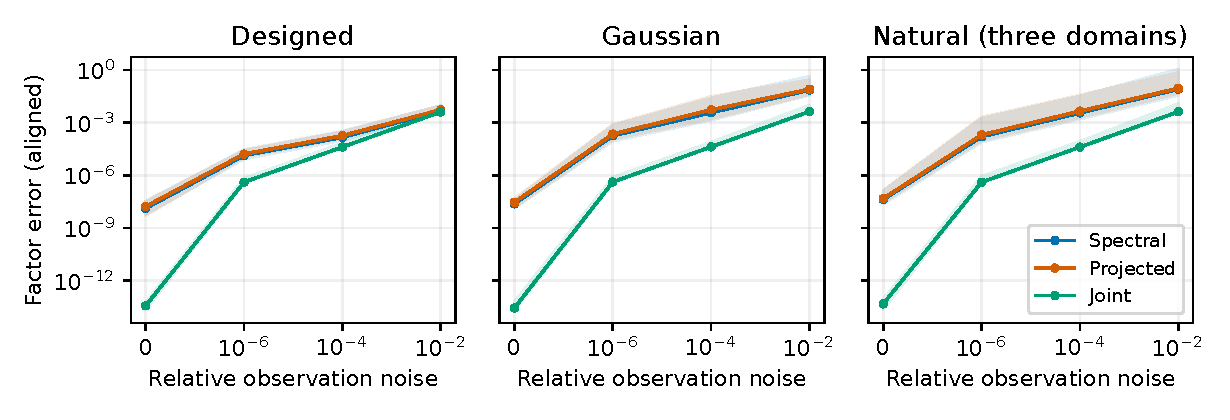
\includegraphics[width=\linewidth]{figures/llm_recovery.pdf}
\caption{Recovery with four queries. Lines show medians and shaded bands
 the 10th--90th percentiles over all 27 checkpoints; the natural panel also
includes all three domains. These are descriptive spreads across correlated
cases, not confidence intervals. Noiseless results use controlled FP64
factor responses, not full-LLM FP64 inference.}
\label{fig:llm-recovery}
\end{figure}

\paragraph{Calibration transfers here, but does not certify recovery.}
Four separate Pythia adapter checkpoints, with general-text validation
queries only, fix acceptance thresholds before held-out recovery scoring.
At error $>0.10$ defined as bad, the combined joint-fit rule accepts all
1,080 sufficient-rank cases with no observed bad output; residual-only
accepts 868, also with none. This sample therefore cannot establish better
bad-case detection by the combined rule. For projected spectral recovery,
 the combined rule accepts 43 bad outputs among 1,056, versus 20 among 1,037
for residual-only; its largest accepted error is $6.19$.
Raw spectral recovery has an all-reject calibrated policy under the strict
simplex gate, even though many of its factor errors are small.
Table~\ref{tab:llm-acceptance} retains all denominators. The earlier synthetic
study also retains a combined-rule accepted-bad fraction of $5.16\%$,
above its $5\%$ target. Neither calibration nor candidate-local diagnostics
replace the theorem's externally specified domain assumptions.

\paragraph{Precision and structural usefulness remain limiting.}
The controlled response formula agrees with autodiff within
$1.62\times10^{-16}$ relative error. Finite-step subtraction is less
reliable: at step $10^{-5}$, FP32 errors range from $0.040$ to $0.102$,
and BF16 errors from $1.00$ to $1.95$. Separately, shrinking the router-rank
margin in learned factors amplifies noisy recovery error by roughly three
orders of magnitude in the registered secondary stress test
(Figure~\ref{fig:llm-conditioning}).

On nine declared checkpoints, balanced hard groups selected from recovered
routers at noise $10^{-4}$ and $10^{-2}$ exactly reproduce the native
router partitions. However, balanced clustering of the effective parameters
also reproduces all nine. Equal-budget refitting and 64 recovery updates
 therefore provide no evidence that coordinate recovery improves this
 decision over the simpler effective-parameter control. Random balanced
 groups worsen general-text NLL after recovery at all nine checkpoints,
while code/math differences have mixed signs. These are token-loss results,
not generation accuracy or realized inference speedups. Detailed action
results, repeated-action numerical controls, costs, and independent CPU
replays are in Appendix~\ref{app:llm-study}.

\section{Discussion and limitations}

Static factors need not be unique, yet a specified optimizer can expose
additional information about their current coordinates. For the finite
softmax-router/shared-basis model, complete Euclidean response identifies
the factors up to permutation on a common full-rank product fiber.
The quantitative reduction controls original factor error on named
nondegenerate domains. Its finite-noisy consequence bounds the whole
feasible set using queries constructed from the observed product, without
requiring the true basis to lie in an estimated subspace.

The guarantee has substantial conditions: known positive Euclidean block
rates and temperature, internal access to the effective product and full
matrix-valued responses, rank and interior margins, and, for the stated
query construction, $D-K\ge L$. The product error must be below a
domain-dependent threshold. The constants are conservative, query
optimality is unproved, and an efficient globally feasible recovery
algorithm is not supplied. Rank loss, proximity to the simplex boundary,
and weak observation directions obstruct stronger uniform conclusions.

The numerical results illustrate these distinctions. Precise controlled
responses permit accurate recovery, while finite arithmetic and noisy
ill-conditioned problems can produce large errors and falsely accepted
estimates. The empirical rejection rule and candidate-local check cannot
replace the global theorem's domain assumptions. No result here identifies
an AdamW trajectory, a historical sharing graph, or a nonlinear
output-mixture model. The pretrained-model study covers one fixed-rank,
64-channel additive module and three dense model families up to 8B;
it does not establish universality across LLM architectures, sizes, or
adapter parameterizations. Family comparisons confound architecture,
pretraining data and, for the selected Qwen3 models, post-training.
The simple effective-parameter control matches the recovered structural
partitions, so this study does not establish an incremental decision or
compression benefit. The useful positive conclusion is specific: finite
optimizer-response information can resolve a static coordinate ambiguity,
with an explicit account of the observations and margins required.


\bibliography{references}
\bibliographystyle{style/iclr2027/iclr2027_conference}

\section*{AI assistance disclosure}

Generative AI tools materially assisted the literature search, theorem and
counterexample exploration, software implementation, experiment execution,
analysis, and manuscript drafting. Automated checks and agent reviews
do not constitute external human peer review. Human authors retain
responsibility for the cited sources, mathematical arguments, code, numerical
artifacts, and final contents. No AI system is listed as an author.
Procedural guidance from Scientific Agent Skills~\citep{kassis2026scientificagentskillslibrary}
informed experimental-design critique and evidence grading; this attribution
is not an independent scientific endorsement of the results.


\appendix
\section{Secondary theoretical statements}
\label{app:secondary-theory-statements}

This section preserves the auxiliary static, recovery, probe, and optimization
statements referenced by the main text.  They are separated from the central
optimizer-response theorem because the static change of basis is SSMF prior
art and the positive results use standard additional assumptions.  Complete
proofs and failure cases follow in Appendix~\ref{app:theory}.

\subsection{Static router-coordinate consequences}

The rows $b_1,\ldots,b_K$ are affinely independent when
$[B,\ones]$ has row rank $K$.

\begin{proposition}[Local form of the SSMF gauge]
\label{thm:continuous_gauge}
Assume $K\ge2$, $A$ is strictly positive and has column rank $K$, and the
rows of $B$ are affinely independent.  For every nonzero
$H\in\RR^{K\times K}$ satisfying $H\ones=0$, and every sufficiently small
$t\ne0$,
\begin{equation}
 M_t=I+tH,\qquad A_t=AM_t,\qquad B_t=M_t^{-1}B
 \label{eq:gauge_path}
\end{equation}
is a valid factorization with $A_t\in\simplex_K^L$, affinely independent
bases, and $A_tB_t=AB$.  It is not permutation equivalent to $(A,B)$.  The
local equivalence class therefore has at least $K(K-1)$ continuous
directions.
\end{proposition}

The condition $H\ones=0$ preserves row sums; positivity and invertibility
survive a small perturbation; and
$[B_t,\ones]=M_t^{-1}[B,\ones]$ preserves affine independence.  Full column
rank of $A$ rules out a hidden permutation.

For $0<s<1$, the gauge
\begin{equation}
 M_s=(1-s)I+s\ones\ones^\top/K
 \label{eq:uniformizing_gauge}
\end{equation}
moves every router row toward uniform and strictly increases its entropy
unless it was already uniform, while $M_s^{-1}B$ keeps $\Theta$ fixed.
This uniformizing path preserves argmax assignments. They are not
invariant under other feasible gauges, however. For example,
\begin{equation}
 A=\begin{bmatrix}.1&.9\\.3&.7\\.4&.6\\.9&.1\end{bmatrix},\qquad
 M=\begin{bmatrix}.9&.1\\.4&.6\end{bmatrix}
 \label{eq:argmax_example}
\end{equation}
gives argmax labels $(2,2,2,1)$ before and $(2,1,1,1)$ after multiplication
by $M$.  Yet $(AM)(M^{-1}B)=AB$ for every $B$.

This ambiguity does not erase every partition statistic.  Because $M$ is
invertible, $a_i=a_j$ iff $a_iM=a_jM$; affine independence of the rows of
$B$ already makes this equivalent to $\theta_i=\theta_j$.  Indeed,
$qB=0$ and $q\ones=0$ imply $q=0$ when $[B,\ones]$ has row rank $K$.

\begin{proposition}[End-to-end impossibility]
\label{thm:end_to_end_impossibility}
Suppose an architecture and its observation law depend on $(A,B)$ only through
$\Theta=AB$.  If two gauge-equivalent factorizations have different router
summaries, no estimator based on end-to-end input--output observations can
recover the correct summary in both worlds.  This remains true with oracle
access to the predictor on every input.
\end{proposition}

This result concerns router coordinates; it neither equates effective-weight
equality with functional equivalence nor asserts that either equals a planted
generative graph.  The latter is independently impossible under composition:
a two-layer linear teacher with $W_1=W_2=I$ (tied) and one with
$W_1=2I,\ W_2=I/2$ (untied) both implement $x\mapsto x$.

\subsection{Positive recovery under additional information}

Call a factorization \emph{separable} if every basis has an anchor layer
$i_j$ with $a_{i_j}=e_j$.

\begin{proposition}[Standard separable recovery]
\label{thm:anchor_recovery}
If two $K$-separable factorizations of the same $\Theta$ have affinely
independent bases, they are permutation equivalent.  Consequently, if routing
is one-hot with discrete label $c_i\in\{1,\ldots,K\}$, every basis is used,
and the bases are affinely independent, then
\begin{equation}
 c_i=c_{i'}\quad\Longleftrightarrow\quad\theta_i=\theta_{i'},
 \label{eq:onehot_partition}
\end{equation}
so the sharing partition is recoverable up to basis relabeling.
\end{proposition}

This is standard separable-SSMF geometry specialized to layer rows, not a new
simplex-identification result~\citep{abdolali2021simplex}.  Separability makes
$\operatorname{conv}\{\theta_i\}$ equal the simplex whose vertices are the
bases; vertices are unique, and affine independence gives unique barycentric
coordinates.  The restriction to the separable model class is essential: an
unrestricted soft factorization may place a larger simplex outside the
observed convex hull.

\begin{theorem}[Stable noisy one-hot recovery]
\label{thm:noisy_recovery}
Assume $K\ge2$.  Suppose $c_i\in\{1,\ldots,K\}$ and
$\widehat\theta_i=b_{c_i}+e_i$, $\|e_i\|_2\le\varepsilon$, and
$\gamma=\min_{j\ne k}\|b_j-b_k\|_2>4\varepsilon$.  Connecting two layers
when their observed parameters are at distance at most $2\varepsilon$
recovers the exact one-hot partition.  Each cluster mean estimates its basis
to error at most $\varepsilon$.
\end{theorem}

Parameter access is not always available.  Shared-input probes instead target
the clean functional partition defined in Section~\ref{sec:problem}.  Let
$Y_i(H)$ be the possibly noisy observation of layer $i$'s residual update on
a common probe.  The result below applies only when the distances induced by
that observation law retain a positive gap for the clean target partition;
layer-dependent noise can destroy this condition.  Define
\begin{equation}
 d_{ij}^2=\mathbb E\|Y_i(H)-Y_j(H)\|_2^2,\qquad
 \widehat d_{ij}^2=\frac1n\sum_{s=1}^n
 \|Y_i(H_s)-Y_j(H_s)\|_2^2.
 \label{eq:probe_distances}
\end{equation}

\begin{theorem}[Finite-probe partition recovery]
\label{thm:probe_recovery}
Let $L\ge2$, let $0<\eta<1$, and suppose the target partition has at least
two classes. Let it have population within-class radius
$w=\max_{i\sim_f j}d_{ij}^2$ and between-class separation
$b=\min_{i\not\sim_f j}d_{ij}^2$, with gap $\delta=b-w>0$.  Suppose the
centered squared-distance observations satisfy, uniformly over layer pairs,
the Bernstein tail
\begin{equation}
 \Pr\!\left(\left|\widehat d_{ij}^2-d_{ij}^2\right|>u\right)
 \le2\exp\!\left[-n\min\!\left\{\frac{u^2}{2\nu^2},
                                      \frac{u}{2c}\right\}\right].
 \label{eq:probe_bernstein}
\end{equation}
If, for failure probability $\eta$,
\begin{equation}
 n\ge
 \max\!\left\{\frac{32\nu^2}{\delta^2},\frac{8c}{\delta}\right\}
 \log\frac{2\binom{L}{2}}{\eta},
 \label{eq:probe_sample_complexity}
\end{equation}
then thresholding $\widehat d_{ij}^2$ at $(w+b)/2$ recovers the functional
partition with probability at least $1-\eta$.  The same strict separation
guarantees recovery by single, complete, or average agglomerative linkage when
the number $K_f$ of functional equivalence classes is known.  In general
$K_f$ need not equal the number $K$ of router bases.
\end{theorem}

The result follows by a union bound and certifies equivalence only under the
specified probe distribution; behavior off its support remains unidentified.

\subsection{Optimization and initialization effects}

Let $G=\nabla_\Theta\mathcal L$.

\begin{proposition}[Factorization-induced dynamics]
\label{prop:factor_dynamics}
For Euclidean gradient flow on unconstrained factors, without factor-specific
regularizers,
\begin{equation}
 \dot\Theta=-G(B^\top B)-(AA^\top)G.
 \label{eq:effective_gradient_flow}
\end{equation}
Gauge-equivalent initializations therefore generally have different effective
parameter trajectories despite identical initial $\Theta$, predictions, and
loss.
\end{proposition}

\begin{proposition}[Softmax saturation]
\label{prop:softmax_saturation}
Let $a_i=\operatorname{softmax}(z_i/\tau)$ and suppose
$\max_j a_{ij}=1-\varepsilon$.  With
$g_i=\nabla_{\theta_i}\mathcal L$,
\begin{equation}
 \|\nabla_{z_i}\mathcal L\|_2
 \le \frac{2\varepsilon}{\tau}\|Bg_i\|_2.
 \label{eq:saturation_bound}
\end{equation}
Thus the instantaneous logit gradient is attenuated as the current router row
approaches the simplex boundary.  This pointwise bound alone does not imply
that an initial argmax graph remains fixed over a finite training trajectory;
the loss gradients, basis norm, and probability margin can all change.
\end{proposition}

These results justify testing gauge-equivalent initializations, final--initial
router movement, and recovery under deliberately wrong initial graphs.  They
do not prove that gradient descent prefers a universal smooth, banded, or
low-entropy structure.  Nor do reconstruction loss or end-to-end accuracy by
themselves identify router coordinates, the effective-weight equality
partition, functional equivalence, or a latent generative graph.

\section{Theory proofs, extensions, and scope}
\label{app:theory}

This appendix gives complete proofs for Section~\ref{sec:theory}.  It also
records edge cases that are easy to lose when a soft router is visualized as a
discrete sharing graph.

\subsection{Static SSMF gauge details}
\label{app:gauge_proof}

The non-identifiability conclusion and the symmetric uniformizing path are
the unconstrained SSMF result of
\citet[Section~IV-A]{vuthanh2023bounded} under
\(X=\Theta^\top\), \(W=B^\top\), and \(H=A^\top\); see
Appendix~\ref{app:literature}.  The proof below only records the direct local
row-sum-preserving extension used to delimit which router summaries change.

\begin{proof}[Proof of Proposition~\ref{thm:continuous_gauge}]
The constraint $H\ones=0$ implies
\begin{equation}
  M_t\ones=(I+tH)\ones=\ones.
  \label{eq:app_rowsum}
\end{equation}
The determinant is continuous and $\det(M_0)=1$, so $M_t$ is invertible for
all sufficiently small $|t|$.  Strict positivity is also an open condition:
because $A$ has finitely many entries and $A_{ij}>0$, there is a neighborhood
of zero in which every entry of $AM_t$ remains positive.  Therefore
\begin{equation}
  A_t\ones=AM_t\ones=A\ones=\ones,
  \qquad A_t>0,
\end{equation}
and $A_t\in\simplex_K^L$.  The effective parameters are unchanged because
\begin{equation}
  A_tB_t=(AM_t)(M_t^{-1}B)=AB.
\end{equation}

\Eqref{eq:app_rowsum} also gives
$M_t^{-1}\ones=\ones$.  Hence the augmented basis matrix satisfies
\begin{equation}
 [B_t,\ones]
 =[M_t^{-1}B,M_t^{-1}\ones]
 =M_t^{-1}[B,\ones].
 \label{eq:app_affine_rank}
\end{equation}
Left multiplication by an invertible matrix preserves row rank, so affine
independence is preserved exactly, not merely infinitesimally.

It remains to rule out a permutation.  If $A_t=AP$ for a permutation matrix
$P$, then $A(M_t-P)=0$.  Since $A$ has column rank $K$, it has a left inverse,
and therefore $M_t=P$.  The identity is the only permutation matrix in a
sufficiently small neighborhood of $I$.  For nonzero $t$ and nonzero $H$,
$M_t\ne I$, yielding a contradiction.  Finally, the linear constraint
$H\ones=0$ supplies $K$ independent equations on $K^2$ entries, so its
solution space has dimension $K(K-1)$.  Full column rank makes these local
directions distinct at $A$.
\end{proof}

Any strictly positive router can be written as a softmax: for fixed
$\tau>0$, take $z_{ij}=\tau\log A_{ij}$, up to an arbitrary additive constant
in each row.  Thus softmax normalization does not eliminate the orbit.

\paragraph{Entropy-changing gauges.}
For $M_s$ in \eqref{eq:uniformizing_gauge}, the eigenvalue along
$\ones$ is one and every eigenvalue orthogonal to $\ones$ is $1-s$; hence it
is invertible for $0<s<1$.  Since
\begin{equation}
  A\frac{\ones\ones^\top}{K}
  =\frac{\ones_L\ones^\top}{K}
  =U,
\end{equation}
we have $AM_s=(1-s)A+sU$.  Strict concavity of Shannon entropy gives
\begin{equation}
 H((1-s)a_i+su)
 \ge(1-s)H(a_i)+sH(u)>H(a_i)
\end{equation}
for every nonuniform $a_i$, because $u$ is the unique entropy maximizer.
The effective parameters remain exactly unchanged after replacing $B$ by
$M_s^{-1}B$.  As $s\uparrow1$, the router can approach uniform while the
basis norm may grow.  A norm penalty can prefer one member of this orbit, but
that is a gauge-fixing optimization convention rather than identification by
the data.

\paragraph{Verification of the argmax counterexample.}
The matrix $M$ in \eqref{eq:argmax_example} is positive, row
stochastic, and has determinant $0.5$.  Direct multiplication gives
\begin{equation}
 AM=
 \begin{bmatrix}
 0.45&0.55\\
 0.55&0.45\\
 0.60&0.40\\
 0.85&0.15
 \end{bmatrix}.
\end{equation}
Thus two layer assignments flip.  If $B$ has two distinct rows, those rows are
affinely independent; \eqref{eq:app_affine_rank} shows that
$M^{-1}B$ remains so.  The example therefore does not rely on collapsed
bases.

\begin{proof}[Proof of Proposition~\ref{thm:end_to_end_impossibility}]
Let $(A,B)$ and $(A',B')$ be the two factorizations.  Gauge equivalence gives
$AB=A'B'=\Theta$.  By assumption, for every input $x$,
\begin{equation}
  F(x;A,B)=F(x;AB)=F(x;A'B')=F(x;A',B').
\end{equation}
The complete input--output process, including its distribution under any
design over inputs, is therefore identical in the two worlds.  Every
possibly randomized estimator has the same output distribution in both
worlds.  If the two target router summaries differ, the estimator cannot equal
both with probability one.  The argument already grants the estimator all
function values, so increasing the sample size cannot repair the failure.
\end{proof}

The proposition assumes that factors enter the architecture only through the
parameter product.  If all nonlinear basis modules are executed separately
and their outputs are mixed, an arbitrary linear change of basis need not
remain in that model class.  No claim for such output-space mixtures follows
from this proof.

\subsection{Optimizer-response stabilizer}
\label{app:response_proofs}

We use the convention of Section~\ref{sec:response_identifiability}.  Set
\begin{equation}
 \lambda_Z=\eta_Z/\tau^2,
 \qquad
 C_i=\operatorname{Diag}(a_i)-a_ia_i^\top,
 \qquad
 H_i=B^\top C_i^2B.
 \label{eq:app_response_notation}
\end{equation}
With rows of the input and output represented as column vectors, the
\((i,j)\) block of \(\mathcal R_{A,B}\) is
\begin{equation}
 [\mathcal R_{A,B}]_{ij}
 =\eta_B(a_i^\top a_j)I_D
  +\mathbf 1\{i=j\}\lambda_ZH_i.
 \label{eq:app_response_blocks}
\end{equation}

\begin{proof}[Proof of Theorem~\ref{thm:response_stabilizer}]
Because both factorizations have rank \(K\), their column spaces equal the
column space of their common product.  Standard full-rank factorization
algebra therefore gives a unique \(M\in\operatorname{GL}(K)\) satisfying
\begin{equation}
 A'=AM,\qquad B'=M^{-1}B.
 \label{eq:app_response_gauge}
\end{equation}
Both routers have unit row sums, so
\(A(M\ones-\ones)=0\).  Full column rank of \(A\) gives
\begin{equation}
 M\ones=\ones.
 \label{eq:app_response_rowsum}
\end{equation}

Equality of the response on every \(G\) is equality of every block in
\eqref{eq:app_response_blocks}.  For \(i\ne j\), it gives
\begin{equation}
 a_i^\top a_j=(a_i')^\top a_j'.
 \label{eq:app_response_offdiag_gram}
\end{equation}
For a diagonal block, define
\(H_i'=(B')^\top(C_i')^2B'\).  Its equality can be rearranged as
\begin{equation}
 H_i-H_i'=c_iI_D,
 \qquad
 c_i=-\frac{\eta_B}{\lambda_Z}
   \bigl(\|a_i\|_2^2-\|a_i'\|_2^2\bigr)
 \label{eq:app_response_scalar_identity}
\end{equation}
for a scalar \(c_i\).  Every simplex covariance satisfies
\(C_i\succeq0\) and \(C_i\ones=0\); full row rank of \(B\) therefore gives
\(H_i\succeq0\) and \(\operatorname{rank}(H_i)\le K-1<D\).  The same holds for
\(H_i'\).  If \(c_i>0\), then \(H_i=H_i'+c_iI_D\) would be positive
definite; if \(c_i<0\), then \(H_i'=H_i-c_iI_D\) would be positive definite.
Both contradict singularity, so \(c_i=0\).  The remaining scalar part of the
diagonal block then gives
\(\|a_i\|_2^2=\|a_i'\|_2^2\).  Together with
\eqref{eq:app_response_offdiag_gram},
\begin{equation}
 AA^\top=A'A'^\top=AMM^\top A^\top.
\end{equation}
Multiplication by a left inverse of \(A\) and its transpose yields
\begin{equation}
 MM^\top=I_K.
 \label{eq:app_response_orthogonal}
\end{equation}

Since \(H_i=H_i'\), substituting \eqref{eq:app_response_gauge} and cancelling
\(B\) with a right inverse gives
\begin{equation}
 C_i^2=M^{-\top}(C_i')^2M^{-1}.
\end{equation}
By \eqref{eq:app_response_orthogonal}, this is
\begin{equation}
 C_i^2=M(C_i')^2M^\top=(MC_i'M^\top)^2.
\end{equation}
Both \(C_i\) and \(MC_i'M^\top\) are positive semidefinite.  Uniqueness of
the positive-semidefinite square root therefore gives
\begin{equation}
 C_i=MC_i'M^\top.
 \label{eq:app_response_jacobian_conjugacy}
\end{equation}

In column convention, \(a_i'=M^\top a_i\).  Expanding
\eqref{eq:app_response_jacobian_conjugacy}, the two rank-one terms cancel and
leave
\begin{equation}
 \operatorname{Diag}(a_i)
 =M\operatorname{Diag}(a_i')M^\top.
 \label{eq:app_response_diagonal_algebra}
\end{equation}
For distinct \(r,s\), the \((r,s)\) entry says
\begin{equation}
 \sum_{\ell=1}^K M_{r\ell}M_{s\ell}a'_{i\ell}=0
 \qquad\text{for every }i.
\end{equation}
The rows of \(A'\) span \(\RR^K\), hence
\(M_{r\ell}M_{s\ell}=0\) for every \(\ell\).  Thus each column of the
orthogonal \(M\) has exactly one nonzero entry, equal to \(+1\) or \(-1\):
\(M\) is a signed permutation.  \Eqref{eq:app_response_rowsum}
removes the negative signs, so \(M=P\) is a permutation matrix.

Conversely, if \(A'=AP\) and \(B'=P^\top B\), then
\(a_i'=P^\top a_i\), \(C_i'=P^\top C_iP\), the router Gram matrix is
unchanged, and
\begin{equation}
 (B')^\top(C_i')^2B'=B^\top C_i^2B.
\end{equation}
Every block in \eqref{eq:app_response_blocks} is therefore unchanged.  This
proves both directions.
\end{proof}

\subsection{A quantitative inverse for the response}
\label{app:response_quantitative}

The exact stabilizer has a linear inverse on any uniformly interior,
well-conditioned, norm-bounded set.  The following constants are explicit so
that the claim is checkable; they are not intended to be numerically tight.
For a linear map between matrix spaces, \(\|\cdot\|_{F\to F}\) denotes the
operator norm induced by the Frobenius norm.

\begin{theorem}[Quantitative optimizer-response stability]
\label{thm:response_stability}
Let \(K\ge2\), \(L\ge K\), and \(D\ge K\).  Let
\(A,A'\in\RR^{L\times K}\) be row-stochastic and let
\(B,B'\in\RR^{K\times D}\).  Suppose
\begin{align}
 \min_{i,j}\{A_{ij},A'_{ij}\}&\ge\alpha>0,
 \label{eq:app_stability_interior}\\
 \sigma_{\min}(A),\sigma_{\min}(A')&\ge s_A>0,
 &
 \sigma_{\min}(B),\sigma_{\min}(B')&\ge s_B>0,
 \label{eq:app_stability_singular}\\
 \|A\|_F,\|A'\|_F&\le L_A,
 &
 \|B\|_F,\|B'\|_F&\le L_B,
 \label{eq:app_stability_norms}\\
 AB&=A'B'.
 \label{eq:app_stability_product}
\end{align}
Both response operators are defined with the same
\(\tau,\eta_Z,\eta_B>0\).  Put
\(\lambda_Z=\eta_Z/\tau^2\) and
\begin{equation}
 \delta=\|\mathcal R_{A,B}-\mathcal R_{A',B'}\|_{F\to F}.
 \label{eq:app_stability_delta}
\end{equation}
Then
\begin{equation}
 \min_{P\in\mathfrak S_K}
 \left(\|A'-AP\|_F^2+\|B'-P^\top B\|_F^2\right)^{1/2}
 \le C\delta,
 \label{eq:app_stability_conclusion}
\end{equation}
where the following is one finite, fully explicit choice.  First define the
factorization and Gram constants
\begin{equation}
 L_M=\max\{1,L_A/s_A\},\qquad
 c_G=\frac{L}{\eta_Bs_A^2},\qquad
 c_H=\frac{2}{\lambda_Zs_B^2}.
 \label{eq:app_stability_constants_gram}
\end{equation}
Next define the covariance and diagonal-algebra constants
\begin{align}
 \mu_*&=\alpha\left(1+\frac{1}{4L_M^2}\right),&
 c_J&=\frac{L_M^2(c_G+c_H)}{\mu_*},&
 c_D&=\frac{\sqrt{LK}}{s_A}c_J.
 \label{eq:app_stability_constants_cov}
\end{align}
Finally define the row-rounding and global constants
\begin{align}
 c_{\rm row}
 &=\left[Kc_D^2+(c_G+Kc_D^2)^2\right]^{1/2},
 \label{eq:app_stability_constants_row}\\
 \delta_0
 &=\min\left\{1,\frac{1}{2c_G},
                    \frac{1}{2\sqrt K\,c_{\rm row}}\right\},
 \label{eq:app_stability_constants_delta0}\\
 C_{\rm loc}
 &=\sqrt{L_A^2+(L_ML_B)^2}\,\sqrt K\,c_{\rm row},&
 C
 &=\max\left\{C_{\rm loc},
       \frac{2\sqrt{L_A^2+L_B^2}}{\delta_0}\right\}.
 \label{eq:app_stability_constants_global}
\end{align}
\end{theorem}

\begin{proof}
Except where a Frobenius norm is displayed explicitly, all matrix norms in
this proof are spectral norms.  We divide the argument into four steps.

\paragraph{Step 1: recovering the router Gram matrix and an almost-orthogonal
gauge.}
Injecting a vector into input block \(j\) and projecting the output onto block
\(i\) are contractions for the Frobenius-induced operator norm.  Therefore
each block of
\(\mathcal R_{A,B}-\mathcal R_{A',B'}\) has spectral norm at most
\(\delta\).  For \(i\ne j\), \eqref{eq:app_response_blocks} gives
\begin{equation}
 \left|(AA^\top-A'A'^\top)_{ij}\right|
 \le\frac{\delta}{\eta_B}.
 \label{eq:app_stability_offdiag}
\end{equation}
For a diagonal block, write
\begin{equation}
 E_i=t_iI_D+\lambda_Z(H_i-H_i'),\qquad
 t_i=\eta_B(\|a_i\|_2^2-\|a_i'\|_2^2),
 \label{eq:app_stability_diagblock}
\end{equation}
where \(H_i'=(B')^\top(C_i')^2B'\).  Both \(H_i\) and \(H_i'\) are singular
positive-semidefinite matrices: their ranks are at most \(K-1<D\).  If
\(t_i\ge0\), evaluating \(E_i\) on a unit vector in
\(\ker(H_i')\) gives a quadratic form at least \(t_i\).  If \(t_i<0\),
evaluating it on a unit vector in \(\ker(H_i)\) gives a quadratic form at most
\(t_i\).  Since \(\|E_i\|_2\le\delta\), in either case
\begin{equation}
 |t_i|\le\delta,\qquad
 \|H_i-H_i'\|_2\le\frac{2\delta}{\lambda_Z}.
 \label{eq:app_stability_diagseparate}
\end{equation}
The diagonal entries of the router Gram difference consequently satisfy the
same bound as \eqref{eq:app_stability_offdiag}, and hence
\begin{equation}
 \|AA^\top-A'A'^\top\|_F\le\frac{L\delta}{\eta_B}.
 \label{eq:app_stability_gram}
\end{equation}

The common product has rank \(K\), so full-rank factorization algebra gives a
unique \(M\in\operatorname{GL}(K)\) with
\begin{equation}
 A'=AM,\qquad B'=M^{-1}B,\qquad M\ones=\ones.
 \label{eq:app_stability_M}
\end{equation}
Moreover,
\begin{equation}
 M=A^\dagger A',\qquad
 M^{-1}=(A')^\dagger A,\qquad
 \|M\|_2,\|M^{-1}\|_2\le L_A/s_A\le L_M.
 \label{eq:app_stability_M_bounds}
\end{equation}
Multiplying \eqref{eq:app_stability_gram} on the left by \(A^\dagger\)
and on the right by \((A^\dagger)^\top\) yields
\begin{equation}
 \|I_K-MM^\top\|_2\le c_G\delta.
 \label{eq:app_stability_almost_orthogonal}
\end{equation}

\paragraph{Step 2: recovering the simplex covariance matrices.}
Let
\(Q=B^\top(BB^\top)^{-1}\).  Then \(BQ=I_K\) and
\(\|Q\|_2\le1/s_B\).  Substitute \(B'=M^{-1}B\) in \(H_i'\), and multiply
\eqref{eq:app_stability_diagseparate} by \(Q^\top\) and \(Q\), to obtain
\begin{equation}
 \|C_i^2-M^{-\top}(C_i')^2M^{-1}\|_2\le c_H\delta.
 \label{eq:app_stability_cov_squares_raw}
\end{equation}
Set \(Y_i=M^\top C_iM\).  The identity
\begin{align}
 Y_i^2-(C_i')^2
 ={}&M^\top C_i(MM^\top-I_K)C_iM \notag\\
 &+M^\top\{C_i^2-M^{-\top}(C_i')^2M^{-1}\}M
 \label{eq:app_stability_cov_squares}
\end{align}
together with \(\|C_i\|_2\le1\),
\eqref{eq:app_stability_M_bounds},
\eqref{eq:app_stability_almost_orthogonal}, and
\eqref{eq:app_stability_cov_squares_raw} gives
\begin{equation}
 \|Y_i^2-(C_i')^2\|_2
 \le L_M^2(c_G+c_H)\delta.
 \label{eq:app_stability_square_bound}
\end{equation}

Strict interiority now supplies the spectral gap that is unavailable near the
simplex boundary.  If \(a\) is a probability vector with
\(\min_j a_j\ge\alpha\), then
\begin{equation}
 C(a)=\operatorname{Diag}(a)-aa^\top
 \succeq\alpha\Pi_{\ones^\perp}.
 \label{eq:app_stability_cov_gap}
\end{equation}
Indeed, write \(a=\alpha\ones+r\), where \(r\ge0\) and
\(\ones^\top r=1-K\alpha\le1\).  For \(x\perp\ones\), weighted
Cauchy--Schwarz gives
\[
 x^\top C(a)x
 =\alpha\|x\|_2^2+\sum_jr_jx_j^2-\left(\sum_jr_jx_j\right)^2
 \ge\alpha\|x\|_2^2.
\]
Both \(Y_i\) and \(C_i'\) have kernel exactly
\(\operatorname{span}\{\ones\}\): for the former, use
\(M^{-1}\ones=\ones\).  They are symmetric, so they preserve
\(\ones^\perp\).  For a unit \(x\perp\ones\), decompose
\(Mx=c\ones+y\), with \(y\perp\ones\).  Since
\(x=c\ones+M^{-1}y\), orthogonality of \(x\) and
\eqref{eq:app_stability_M_bounds} imply
\begin{equation}
 |c|\sqrt K\le L_M\|y\|_2,\qquad
 1\le |c|\sqrt K+L_M\|y\|_2,
\end{equation}
and therefore \(\|y\|_2\ge1/(2L_M)\).  It follows from
\eqref{eq:app_stability_cov_gap} that, on \(\ones^\perp\),
\begin{equation}
 Y_i\succeq\frac{\alpha}{4L_M^2}I,
 \qquad C_i'\succeq\alpha I.
 \label{eq:app_stability_two_gaps}
\end{equation}

On this subspace put \(D_i=Y_i-C_i'\).  The Sylvester equation
\begin{equation}
 Y_iD_i+D_iC_i'=Y_i^2-(C_i')^2
\end{equation}
has the integral solution
\begin{equation}
 D_i=\int_0^\infty
 e^{-tY_i}\{Y_i^2-(C_i')^2\}e^{-tC_i'}\,dt.
\end{equation}
The two lower bounds in \eqref{eq:app_stability_two_gaps} show that the norm of
this inverse is at most \(1/\mu_*\).  Both sides vanish on
\(\operatorname{span}\{\ones\}\), so \eqref{eq:app_stability_square_bound}
proves on the whole space that
\begin{equation}
 \|M^\top C_iM-C_i'\|_2\le c_J\delta.
 \label{eq:app_stability_cov_linear}
\end{equation}
The shared exact kernel is what permits a linear estimate here; a generic
perturbation bound for square roots would only be H\"older of order one half.

\paragraph{Step 3: approximately normalizing the diagonal algebra.}
Because \(a_i'=M^\top a_i\), expanding the two covariance matrices in
\eqref{eq:app_stability_cov_linear} cancels their rank-one terms and gives
\begin{equation}
 \|M^\top\operatorname{Diag}(a_i)M-\operatorname{Diag}(a_i')\|_2
 \le c_J\delta.
 \label{eq:app_stability_diagonal_algebra}
\end{equation}
Let \(\operatorname{Off}(X)\) set the diagonal of \(X\) to zero, let
\(E_{jj}=e_je_j^\top\), and define
\(X_j=\operatorname{Off}(M^\top E_{jj}M)\).  Taking the off-diagonal part is
contractive in Frobenius norm, while
\(\|X\|_F\le\sqrt K\|X\|_2\).  Thus
\eqref{eq:app_stability_diagonal_algebra} implies
\begin{equation}
 \left\|\sum_{j=1}^K A_{ij}X_j\right\|_F
 \le\sqrt K\,c_J\delta
 \qquad(1\le i\le L).
 \label{eq:app_stability_linear_system}
\end{equation}
Apply row \(j\) of \(A^\dagger\) to this system in the direct-sum Frobenius
space.  That row has Euclidean norm at most \(1/s_A\); Cauchy--Schwarz over
the \(L\) rows gives
\begin{equation}
 \|\operatorname{Off}(M^\top E_{jj}M)\|_F
 \le c_D\delta
 \qquad(1\le j\le K).
 \label{eq:app_stability_off_bound}
\end{equation}

\paragraph{Step 4: rounding the gauge to a permutation.}
Write \(M^\top E_{jj}M=r_jr_j^\top\), where \(r_j^\top\) is row \(j\) of
\(M\), and choose \(q\) maximizing \(|r_{jq}|\).  Suppose first that
\(\delta\le\delta_0\).  From
\eqref{eq:app_stability_almost_orthogonal},
\(\|r_j\|_2^2\ge1/2\), so \(r_{jq}^2\ge1/(2K)\).  The squared Frobenius norm
in \eqref{eq:app_stability_off_bound} contains
\(2r_{jq}^2\sum_{\ell\ne q}r_{j\ell}^2\).  Consequently
\begin{align}
 \sum_{\ell\ne q}r_{j\ell}^2
 &\le Kc_D^2\delta^2,
 \label{eq:app_stability_row_tail}\\
 |r_{jq}^2-1|
 &\le(c_G+Kc_D^2)\delta.
 \label{eq:app_stability_row_peak}
\end{align}
The second inequality also uses \(\delta\le1\).  Equations
\eqref{eq:app_stability_row_tail}--\eqref{eq:app_stability_row_peak} show that
row \(j\) is within \(c_{\rm row}\delta\) of a signed coordinate vector.

Collect the selected signed coordinate rows into a matrix \(S\).  By
\eqref{eq:app_stability_constants_delta0},
\begin{equation}
 \|M-S\|_2\le\|M-S\|_F
 \le\sqrt K\,c_{\rm row}\delta\le\frac12.
 \label{eq:app_stability_rounding}
\end{equation}
If two rows selected the same coordinate, \(S\) would be singular and
\(\sigma_{\min}(M)\le1/2\).  This contradicts
\eqref{eq:app_stability_almost_orthogonal}, which gives
\(\sigma_{\min}(M)\ge1/\sqrt2\).  The selected coordinates are therefore
distinct.  Each row of \(M\) sums to one by \eqref{eq:app_stability_M}.  Its
distance from any negative coordinate vector is consequently at least
\(2/\sqrt K\), whereas its selected-row distance in
\eqref{eq:app_stability_rounding} is at most \(1/(2\sqrt K)\).  Every sign is
positive, so \(S=P\) is a permutation matrix and
\begin{equation}
 \|M-P\|_F\le\sqrt K\,c_{\rm row}\delta.
 \label{eq:app_stability_permutation}
\end{equation}

Now
\[
 \|A'-AP\|_F\le L_A\|M-P\|_F.
\]
Using
\(M^{-1}-P^\top=M^{-1}(P-M)P^\top\) also gives
\[
 \|B'-P^\top B\|_F
 \le L_ML_B\|M-P\|_F.
\]
These two bounds and \eqref{eq:app_stability_permutation} prove
\eqref{eq:app_stability_conclusion} with \(C_{\rm loc}\) whenever
\(\delta\le\delta_0\).  If \(\delta\ge\delta_0\), choosing the identity
permutation and using the parameter-set diameter gives
\[
 \left(\|A'-A\|_F^2+\|B'-B\|_F^2\right)^{1/2}
 \le2\sqrt{L_A^2+L_B^2}
 \le\frac{2\sqrt{L_A^2+L_B^2}}{\delta_0}\delta.
\]
Taking the larger of the local and diameter constants completes the proof.
\end{proof}

\paragraph{Why the quantitative assumptions appear.}
The exact product constraint \eqref{eq:app_stability_product} cannot be
replaced by response closeness alone: \((A,B)\) and \((A,-B)\) have identical
responses but opposite effective matrices.  The two singular-value margins
keep the factorization gauge and the right inverse of \(B\) bounded.  The
interior margin creates the uniform covariance gap in
\eqref{eq:app_stability_cov_gap}; without it, the inverse can become
arbitrarily ill-conditioned near a simplex face.  Norm bounds make the
nonlocal diameter argument finite.  Finally, using the same temperature and
block rates is part of specifying the optimizer metric rather than a
technical normalization.  These assumptions are sufficient and transparent,
not asserted to be jointly minimal.

Here are three explicit degenerating families showing that a uniform linear
constant cannot ignore the interior or either rank margin.  They also make
clear that these are stability failures, not counterexamples to the exact
theorem.  Set \(K=L=D=3\), \(U=\ones\ones^\top/3\), and
\begin{equation}
 Q=\frac13
 \begin{bmatrix}
  2&-1&2\\[-1mm]
  -1&2&2\\[-1mm]
  2&2&-1
 \end{bmatrix}.
 \label{eq:app_stability_fixed_Q}
\end{equation}
Then \(Q\) is a non-permutation orthogonal matrix and \(Q\ones=\ones\).

\emph{Router-rank margin.}
For \(0<\varepsilon\le1/4\), let
\[
 A_\varepsilon=U+\varepsilon(I-U),\quad B_\varepsilon=I,\qquad
 A_\varepsilon'=A_\varepsilon Q,\quad B_\varepsilon'=Q^\top .
\]
Both routers are strictly positive, the basis singular values equal one, and
all norms and entrywise interior margins remain uniformly bounded.  However,
\(\sigma_{\min}(A_\varepsilon)=
\sigma_{\min}(A_\varepsilon')=\varepsilon\).
The products and router Gram matrices agree exactly.  At
\(\varepsilon=0\), every router row is uniform and
\(C_i=(I-U)/3\), which commutes with \(Q\); hence the local response terms
also agree.  Define the permutation-orbit distance \(d_\varepsilon\) by
\[
 d_\varepsilon^2
 =\min_P\left\{
   \|A_\varepsilon'-A_\varepsilon P\|_F^2+
   \|B_\varepsilon'-P^\top B_\varepsilon\|_F^2\right\}.
\]
Polynomial dependence on \(\varepsilon\) gives
\begin{align}
 \|\mathcal R_{A_\varepsilon,B_\varepsilon}
       -\mathcal R_{A_\varepsilon',B_\varepsilon'}\|_{F\to F}
 &=O(\varepsilon),\\
 d_\varepsilon&\longrightarrow \min_P\|Q-P^\top\|_F>0.
\end{align}
Thus no uniform inverse constant survives as \(s_A\downarrow0\).

\emph{Basis-rank margin.}
Keep \(Q\) from \eqref{eq:app_stability_fixed_Q}, put
\[
 A=0.3\ones\ones^\top+0.1I,\quad A'=AQ,\qquad
 B_\varepsilon=\ones e_1^\top+\varepsilon I,\quad
 B_\varepsilon'=Q^\top B_\varepsilon .
\]
The routers have fixed positive entries and fixed full rank; all norms remain
bounded, while \(\sigma_{\min}(B_\varepsilon)\to0\).
Because \(C_i\ones=C_i'\ones=0\), all cross terms with
\(\ones e_1^\top\) vanish and
\[
 B_\varepsilon^\top C_i^2B_\varepsilon=\varepsilon^2C_i^2,\qquad
 (B_\varepsilon')^\top(C_i')^2B_\varepsilon'
 =\varepsilon^2Q(C_i')^2Q^\top .
\]
The Gram parts again agree exactly, so the response difference is
\(O(\varepsilon^2)\).  The parameter distance tends to the strictly positive
distance between \(A'=AQ\) and the finite permutation orbit of the full-rank
\(A\).  Hence the constant must also deteriorate as \(s_B\downarrow0\).

\emph{Interior margin.}
Let
\[
 S=\frac1{\sqrt3}
 \begin{bmatrix}0&-1&1\\1&0&-1\\-1&1&0\end{bmatrix},\qquad
 Q_t=\exp(tS),
 \]
and, for sufficiently small \(t>0\), set
\[
 A_t=t\ones\ones^\top+(1-3t)I,\quad B_t=I,\qquad
 A_t'=A_tQ_t,\quad B_t'=Q_t^\top .
\]
Here \(S^\top=-S\) and \(S\ones=0\), so \(Q_t\) is orthogonal and fixes
\(\ones\).  Moreover
\(A_t'=I+t(\ones\ones^\top-3I+S)+O(t^2)\); its off-diagonal
first-order coefficients are \(1\pm1/\sqrt3>0\).  Thus both routers are
strictly positive for all sufficiently small \(t\), while their minimum entry
is \(\Theta(t)\).  Their smallest singular values are
\(1-3t\), and both basis singular values equal one, so every rank and norm
margin stays uniform.  The products and Gram responses agree exactly.  Each
row tends to a simplex vertex, so
\(C(a_{t,i})=O(t)\) and \(C(a_{t,i}')=O(t)\); consequently the remaining
squared-covariance response difference is \(O(t^2)\). For the first row,
direct expansion gives
$\operatorname{tr}(C(a_{t,1})^2)=10t^2+O(t^3)$ and
$\operatorname{tr}(C(a'_{t,1})^2)=12t^2+O(t^3)$.
Orthogonal conjugation preserves trace, so this block's difference has
spectral norm at least $(2/3)t^2+O(t^3)$ before the fixed positive
$\lambda_Z$ multiplier. The full response gap is therefore $\Theta(t^2)$.
On the other hand,
the identity is the nearest permutation for small \(t\), and
\(\|Q_t-I\|_F=\sqrt2\,t+O(t^2)\), so the parameter-orbit distance is
\(\Theta(t)\).  The ratio of parameter distance to response error therefore
diverges like \(1/t\).  This supplies the claimed simplex-face
ill-conditioning while \(s_A,s_B,L_A,L_B\) remain controlled.

\subsection{Finite structured response tomography}
\label{app:response_tomography}

We now prove Corollary~\ref{cor:response_tomography}.  Write

\[
 Q=AA^\top,
 \qquad
 T_i=\lambda_Z B^\top C_i^2B,
 \qquad
 S=\operatorname{row}(\Theta).
\]
Under the rank hypotheses, $\operatorname{rank}(\Theta)=K$ and

\begin{equation}
 S=\operatorname{row}(B),\qquad
 \operatorname{range}(T_i)\subseteq S,\qquad
 T_i x=0\ \text{for every }x\in S^\perp.
 \label{eq:app_tomo_support}
\end{equation}
Indeed, a left inverse of $A$ gives
$B=A^\dagger\Theta$, while $\Theta=AB$ gives the reverse row-space
inclusion; the remaining claims follow from the two outer factors $B^\top$
and $B$ in $T_i$.

Choose $u_1,\ldots,u_K$ and $v_1,\ldots,v_L$ as in the corollary and
define the rows of the $K$ probes by
\begin{equation}
 g_j^{(1)}=v_j+u_1,\qquad
 g_j^{(r)}=u_r\quad(2\le r\le K).
 \label{eq:app_tomo_probes}
\end{equation}
Let $y_i^{(r)}=[\mathcal R_{A,B}(G^{(r)})]_i$.  Then
\begin{align}
 Q_{ij}
 &=\eta_B^{-1}\langle y_i^{(1)},v_j\rangle,
 \label{eq:app_tomo_Q}\\
 T_i u_1
 &=y_i^{(1)}-\eta_B\sum_{j=1}^LQ_{ij}(v_j+u_1),
 \label{eq:app_tomo_local_first}\\
 T_i u_r
 &=y_i^{(r)}-\eta_B\left(\sum_{j=1}^LQ_{ij}\right)u_r,
 \qquad 2\le r\le K.
 \label{eq:app_tomo_local_later}
\end{align}

\begin{proof}[Proof of Corollary~\ref{cor:response_tomography}]
Project the first response onto $S^\perp$.  By
\eqref{eq:app_tomo_support},
\[
 \Pi_{S^\perp}y_i^{(1)}=\eta_B\sum_{j=1}^LQ_{ij}v_j.
\]
Taking its inner product with $v_j$ gives
\eqref{eq:app_tomo_Q}.  Subtracting the now-known shared term from the
unprojected response leaves
$T_i(v_i+u_1)=T_i u_1$, proving
\eqref{eq:app_tomo_local_first}.  For probe $r\ge2$, the same subtraction
leaves $T_i u_r$, which proves \eqref{eq:app_tomo_local_later}.

For every $x\in\RR^D$, \Eqref{eq:app_tomo_support} gives
\[
 T_i x=\sum_{r=1}^K\langle u_r,x\rangle T_i u_r.
\]
Thus Equations~\ref{eq:app_tomo_Q}--\ref{eq:app_tomo_local_later} recover $Q$
and every complete local block $T_i$, and \eqref{eq:response_blocks}
then determines the whole response operator.  Two exact charts of the same
rank-$K$ product have the same $S$, so the same probes recover both
operators.  Equality on those probes is therefore equivalent to equality of
the complete responses, and Theorem~\ref{thm:response_stabilizer} gives the
permutation conclusion and its converse.  The $Z$-level row shifts remain
unobserved.
\end{proof}

The complement-code solve in \eqref{eq:app_tomo_Q} and the $S$-coordinate
solves use orthonormal systems and have condition number one.  That statement
concerns recovery of $Q,T_1,\ldots,T_L$ from response observations; it does
not remove the rank and simplex-boundary conditioning in the inverse from
these components back to the factor chart.

\begin{proposition}[Deterministic observation-noise propagation]
\label{prop:response_tomography_noise}
Suppose the observed response to probe $r$ is
$Y^{(r)}+E^{(r)}$, where
$\|E^{(r)}\|_F\le\epsilon_r$, and use
Equations~\ref{eq:app_tomo_Q}--\ref{eq:app_tomo_local_later} for reconstruction.
Then
\begin{equation}
 \|\widehat Q-Q\|_F\le\epsilon_1/\eta_B.
 \label{eq:app_tomo_noise_Q}
\end{equation}
If $T^{(S)}$ stacks the $K\times K$ matrices representing every $T_i$
in the $u$ basis, then
\begin{equation}
 \|\widehat T^{(S)}-T^{(S)}\|_F
 \le\left[(1+\sqrt{L+1})^2\epsilon_1^2+
 \sum_{r=2}^K(\epsilon_r+\sqrt L\epsilon_1)^2\right]^{1/2}.
 \label{eq:app_tomo_noise_local}
\end{equation}
\end{proposition}

\begin{proof}
Right multiplication by the orthonormal-row complement-code matrix is
nonexpansive, which proves \eqref{eq:app_tomo_noise_Q}.  The first probe has
$G^{(1)}(G^{(1)})^\top=I_L+\ones\ones^\top$, hence
$\|G^{(1)}\|_2=\sqrt{L+1}$.  The error in the reconstructed first local
column is therefore at most
\[
 \epsilon_1+\eta_B\|\widehat Q-Q\|_F\|G^{(1)}\|_2
 \le(1+\sqrt{L+1})\epsilon_1.
\]
For every later probe, the erroneous shared subtraction contributes at most
$\eta_B\|(\widehat Q-Q)\ones\|_2\le\sqrt L\epsilon_1$, in addition to
$\epsilon_r$.  Projection into the orthonormal $u$ basis is nonexpansive;
squaring and summing these $K$ column bounds proves
\eqref{eq:app_tomo_noise_local}.
\end{proof}

This gives deterministic error radii, not a noisy ``if and only if.''  Two
noisy reconstructions can be separated when their component gap exceeds the
sum of the applicable radii.  Biased, unknown, or optimizer-state-dependent
observation error requires a different model.

\paragraph{Constructive exact factor recovery.}
The diagonal-algebra reduction also yields an explicit reconstruction once
$Q$ and the local blocks are known. Let $U\in\RR^{K\times D}$ contain the
orthonormal row-space basis, factor $Q=XX^\top$ with $X$ full column rank,
and put $C=X^\dagger\Theta U^\top$. There is an orthogonal $O$ with
$X=AO$, so $C=O^\top BU^\top$ is invertible. Writing
$T_i^{(S)}=UT_iU^\top$ and $x_i=X_{i,:}^\top$, define
\[
 D_i=\left[C^{-\top}(T_i^{(S)}/\lambda_Z)C^{-1}\right]^{1/2}
       +x_ix_i^\top
     =O^\top\operatorname{diag}(a_i)O,
\]
where the square root is the PSD one. A weighted sum of these symmetric
matrices has distinct eigenvalues whenever the weighted sums of the columns
of $A$ are distinct. Full column rank makes those columns distinct, so
continuous Gaussian weights satisfy this condition almost surely. If $V$
is the resulting orthogonal eigenvector matrix, the diagonals of $V^\top D_iV$
recover router rows up to one common permutation; eigenvector signs cancel.
The basis then follows from $\widehat B=\widehat A^\dagger\Theta$.
This is a constructive use of established joint-diagonalization algebra
\citep{afsari2008sensitivity,bhaskara2014uniqueness}, not an additional
uniqueness claim. Its numerical implementation symmetrizes observations and
clips negative eigenvalues before taking square roots. Such clipping, and
the conditioning of a chosen weighted eigensystem, require separate analysis
under noise; the exact argument is not a stability guarantee for that estimator.

\begin{proposition}[Generic probes for the structured response]
\label{prop:response_tomography_gaussian}
Let $p=D-K\ge1$, retain the exact product and rank assumptions above, and
draw $q$ effective-gradient matrices independently with iid standard
Gaussian entries.  If
\begin{equation}
 q\ge\max\left\{K,\left\lceil\frac{L}{p}\right\rceil\right\},
 \label{eq:app_tomo_gaussian_count}
\end{equation}
then their full response vectors determine $Q,T_1,\ldots,T_L$, and hence
the complete structured response, with probability one.
\end{proposition}

\begin{proof}
Express each probe in fixed orthonormal coordinates for $S\oplus S^\perp$.
Concatenate the $S^\perp$ input coordinates over all probes into
$X_\perp\in\RR^{L\times qp}$.  The corresponding projected responses obey
$Y_\perp=\eta_BQX_\perp$.  When $qp\ge L$, the Gaussian matrix
$X_\perp$ has row rank $L$ almost surely, so it determines $Q$.  After
subtracting that shared term, the $q$ input coordinates in $S$ for any
fixed layer form a Gaussian $K\times q$ matrix.  It has row rank $K$
almost surely when $q\ge K$, and therefore determines that layer's local
block.  Taking a finite union over layers preserves probability one.
\end{proof}

At the released dimensions $(L,K,D)=(12,4,787{,}712)$, four complete
Gaussian probe/response vectors would satisfy
\eqref{eq:app_tomo_gaussian_count} almost surely if the rank solves were
actually retained and checked.  The older eight-probe artifacts retain norm
comparisons rather than a tomographic reconstruction, so they remain a
fixed-alternative test. The original four-probe artifact instead executes the
explicit design \eqref{eq:app_tomo_probes}, evaluates the analytic full-
dimensional response, and records the reconstruction residuals.  It does not
run four full-model autograd/JVP queries; the analytic formula is validated
separately on the declared $4\times32$ extraction.
The additive audit in Table~\ref{tab:autograd-tomography} measures all four
full-dimensional responses by reverse automatic differentiation followed by
a forward-mode JVP of the packed factor map. It checks reconstruction on
two unseen directions per chart and records deterministic noise-bound
diagnostics. These queries use linear objectives on the packed parameters;
they do not differentiate the language-model task loss or an AdamW update.

This finite observation result is a structured operator-probing corollary,
not an independent central innovation.  In particular,
\citet[Sec.~3.3, Eqs.~(7)--(9)]{novak2022fast} reconstruct a finite NTK from
identity NTK--vector products; generic and structured matrix probing is
developed by \citet{chiu2012matrix}, \citet{halikias2024structured}, and
\citet{amsel2026query}.  Relative to a generic $LD$-dimensional identity
reconstruction, Equations~\ref{eq:app_tomo_probes}--\ref{eq:app_tomo_local_later}
only exploit the present model's known support and shared-block structure to
compress the queries.

Several boundaries are essential.  The packing condition $D-K\ge L$ is
sufficient for the explicit construction, not a lower bound for all finite
designs.  When $K=1$, the single probe recovers the shared response and the
softmax local blocks vanish.  Exact common product is required because both
charts must share $S$; a small numerical product residual alone gives no
row-space perturbation theorem.  The implementation accordingly activates the
common-design conclusion only for charts produced by an explicit exact
invertible gauge, with the floating-point product residual recorded separately.
Known $\eta_B>0$ is used in \eqref{eq:app_tomo_Q}; known $\eta_Z>0$ and
temperature remain part of the chart theorem.  Finally, these interventions
are executable through linear checkpoint objectives
$\mathcal L_G(\Theta)=\langle G,\Theta\rangle$, but they need not occur in a
natural minibatch trajectory.

\begin{proposition}[Finite Gaussian probes for a fixed response alternative]
\label{prop:response_gaussian_probes}
Let \(m=LD\), represent a fixed nonzero response difference by
\(\mathsf D\in\RR^{m\times m}\), and draw independent
\(x_1,\ldots,x_q\sim\mathcal N(0,I_m)\).  For every \(0<t<1\),
\begin{equation}
 \Pr\left[
   \max_{\ell\le q}\|\mathsf D x_\ell\|_2
   <t\|\mathsf D\|_2
 \right]
 \le[2\Phi(t)-1]^q.
 \label{eq:app_response_small_ball}
\end{equation}
Thus failure probability at most \(\beta\) is obtained when
\begin{equation}
 q\ge
 \frac{\log(1/\beta)}{-\log(2\Phi(t)-1)}.
 \label{eq:app_response_probe_count}
\end{equation}
At \(t=1/2\), the coefficient is approximately \(1.04\).
This is a fixed-alternative, absolute-threshold statement.  It neither
calibrates a relative numerical threshold nor uniformly certifies equality
of arbitrary response operators when \(q<m\).
\end{proposition}

\begin{proof}
Let \(v\) be a unit right singular vector for the largest singular value of
\(\mathsf D\).  An SVD gives
\(\|\mathsf D x\|_2\ge\|\mathsf D\|_2|v^\top x|\), and
\(v^\top x\sim\mathcal N(0,1)\).  Independence across probes proves
\eqref{eq:app_response_small_ball}; solving the right-hand side for \(q\)
gives \eqref{eq:app_response_probe_count}.

For the uniform limitation, after any \(q<m\) realized probes there exists a
nonzero linear map whose kernel contains their span, so all its observed
responses vanish.  Conversely, \(m\) noiseless Gaussian probes form an
invertible \(m\times m\) probe matrix almost surely and therefore determine an
arbitrary response operator.  Finally, a reported ratio such as
\(\|\mathsf D x\|_2/\max\{\|\mathcal R x\|_2,\|\mathcal R'x\|_2\}\) has a
random denominator; \eqref{eq:app_response_small_ball} does not calibrate it
without additional bounds on those response norms.
\end{proof}

\begin{corollary}[Pointwise probe detection from inverse stability]
\label{cor:response_inverse_gaussian}
Fix two exact product-equivalent charts in one nondegenerate set from
Corollary~\ref{cor:response_stability}, fix them before drawing the probes,
and let $C$ be that set's common inverse constant.  Define
\[
 d_{\rm orb}=\min_{P\in\mathfrak S_K}
 \left(\|A'-AP\|_F^2+\|B'-P^\top B\|_F^2\right)^{1/2}
\]
and $\mathsf D=\mathcal R_{A,B}-\mathcal R_{A',B'}$.  If
$d_{\rm orb}\ge\Delta>0$, then independent standard-Gaussian probes satisfy,
for every $0<t<1$,
\begin{equation}
 \Pr\left[
   \max_{\ell\le q}\|\mathsf D x_\ell\|_2
   \ge t\Delta/C
 \right]
 \ge 1-[2\Phi(t)-1]^q.
 \label{eq:app_response_inverse_small_ball}
\end{equation}
\end{corollary}

\begin{proof}
The inverse bound gives $\|\mathsf D\|_2\ge d_{\rm orb}/C\ge\Delta/C$.
The complement of the event in
\eqref{eq:app_response_inverse_small_ball} is therefore contained in the
small-ball event of Proposition~\ref{prop:response_gaussian_probes}, which
proves the claim.
\end{proof}

At $t=1/2$ and $q=8$, the upper bound on the miss probability is about
$4.62\times10^{-4}$.  This number does not calibrate the released relative
response ratios: the threshold $t\Delta/C$ is absolute, $C$ may be loose,
the alternative and common nondegenerate set must be fixed before the draws,
and the statement is not simultaneous over probe-selected charts.  If each
observed difference has deterministic error at most $\epsilon$, the
corresponding observable lower threshold is only
$t\Delta/C-\epsilon$ when positive.

\paragraph{Why the hypotheses and target matter.}
The following examples separate exact theorem hypotheses from broader
interpretations.
\begin{itemize}
 \item Equality of the effective model is indispensable.  With \(A'=A\) and
 \(B'=-B\), the router Gram and every quadratic matrix
 \(B^\top C_i^2B\) are unchanged, but \(A'B'=-AB\).  The response alone does
 not identify the represented effective matrix.

 \item Router rank cannot be dropped.  For \(K=D=3\), let every row of
 \(A\) be \(\ones^\top/3\), let \(B=I_3\), and let \(Q\) be a
 non-permutation orthogonal rotation on \(\ones^\perp\) with
 \(Q\ones=\ones\).  Then \(A'=AQ=A\), \(B'=Q^\top\), and both the product
 and response are unchanged.  The two factors are not permutation
 equivalent.

 \item Basis rank cannot be dropped.  Let
 \(K=D=3\),
 \(A=0.3\ones\ones^\top+0.1I_3\), and
 \(B=\ones e_1^\top\).  For a sufficiently small non-permutation orthogonal
 rotation \(Q\) fixing \(\ones\), \(A'=AQ\) remains positive and
 row-stochastic, while \(B'=Q^\top B=B\).  The products and router Gram
 matrices agree, and \(C_iB=0\) makes every local softmax response term zero.

 \item Joint router training is material in general.  If \(\eta_Z=0\) and
 \(K\ge3\), choose any
 positive full-rank router \(A\) close enough to uniform, a full-row-rank
 \(B\), and a small non-permutation orthogonal \(Q\) fixing \(\ones\).
 Then \((AQ,Q^\top B)\) is valid and product equivalent, while the remaining
 response \(\eta_BAA^\top G\) is unchanged.

 \item Equality on one task gradient is not operator equality.  At a
 stationary point the observed gradient is zero for every parameterization,
 regardless of whether their response operators differ.  There is also a
 nonzero blind direction away from stationarity.  For a non-permutation exact
 full-rank pair with common row space $S$, suppose $D>K$ and $L>2K$.
 Choose nonzero $v\in S^\perp$.  Since
 $\operatorname{rank}(AA^\top-A'(A')^\top)\le2K<L$, choose nonzero
 $w$ in its kernel and set the rows of $G$ to $g_j=w_jv$.  Both local
 block differences kill $v$, while the shared difference kills $w$, so
 $(\mathcal R_{A,B}-\mathcal R_{A',B'})(G)=0$ even though the two response
 operators differ by Theorem~\ref{thm:response_stabilizer}.  A passive
 trajectory probes only its realized directions.

 \item Strict positivity is automatic for finite softmax logits.  The exact
 algebra above in fact only needs each router row to lie in the closed simplex:
 positive semidefiniteness and \(C_i\ones=0\) make \(H_i\) singular.  Thus
 the formula-defined response theorem extends to boundary rows when all stated
 factor ranks remain full.  A uniform interior margin is material only for a
 quantitative inverse bound.
\end{itemize}
These are sufficient conditions, not a claim of a jointly minimal assumption
set.  In particular, the proof uses \(\eta_B>0\) to recover the router Gram
matrix, but we have not established that \(\eta_B>0\) is necessary once the
complete collection of local softmax terms is available.

\paragraph{Partial audit of the \(\eta_B=0\) boundary.}
Among the partial subcases closed in the released assumption ledger, we state
two simple ones here without promoting them to separate contributions.  Write
an equivalent chart as
\(A'=AM\), \(B'=M^{-1}B\), with \(M\ones=\ones\).  For a router row written
as a column \(p\), put \(q=M^\top p\).  Equality of the remaining local blocks
reduces, after cancelling the full-row-rank basis, to
\begin{equation}
 C(q)^2=M^\top C(p)^2M.
 \label{eq:app_etaB_zero_local}
\end{equation}
If \(M\ge0\), define
\(\mathsf K=\operatorname{Diag}(p)M\operatorname{Diag}(q)^{-1}\).
Then \(\ones^\top\mathsf K=\ones^\top\), and
\eqref{eq:app_etaB_zero_local} is equivalent to
\[
 (\mathsf K-p\ones^\top)^\top(\mathsf K-p\ones^\top)
 =(I-q\ones^\top)^\top(I-q\ones^\top).
\]
Thus every two columns of \(\mathsf K\) are at distance \(\sqrt2\).
They also lie in the probability simplex, whose diameter \(\sqrt2\) is
attained only by distinct vertices.  Hence \(\mathsf K=P\); using
\(\mathsf Kq=p\) in its definition gives \(M=P\).  One positive router row
therefore rules out every non-permutation nonnegative gauge.

For \(K=2\), no sign restriction is needed.  Up to a candidate column swap,
write
\(M=\left[\begin{smallmatrix}x&1-x\\y&1-y\end{smallmatrix}\right]\)
with \(d=x-y>0\).  A row \((p,1-p)\) maps to first coordinate
\(q=y+dp\), and \eqref{eq:app_etaB_zero_local} becomes
\(q(1-q)=d p(1-p)\).  Full router rank supplies two distinct
\(p_1<p_2\).  Subtracting the two equations gives
\(q_1+q_2=p_1+p_2=:S\); adding them and using
\(q_2-q_1=d(p_2-p_1)=d\Delta\) gives
\[
 0=\frac{1-d}{2}\{S(2-S)+d\Delta^2\}.
\]
The bracket is positive, so \(d=1\), \(y=0\), and \(M=I\), before undoing
the possible column swap.  For signed gauges with \(K\ge3\), even when both
\(A\) and \(AM\) are positive and full rank, compatibility of the rowwise
regular-simplex congruences remains unresolved.  Numerical searches that
collapse rank, approach a simplex face, or satisfy only one row are not
treated as a proof or counterexample.  We therefore retain \(\eta_B>0\) in
the main theorem while making no necessity claim.

The theorem is specific to the named Euclidean metric and known block rates.
Natural gradient, Adam/AdamW or momentum state, finite optimizer steps,
factor-specific penalties, and router auxiliary losses define different
response objects.  Most importantly, \((\Theta,\mathcal R)\) identifies a
present optimizer chart, not the factors or graph that historically generated
the data.

\subsection{Positive recovery results}
\label{app:positive_proofs}

\begin{lemma}[Unique barycentric coordinates]
\label{lem:app_barycentric}
If $b_1,\ldots,b_K$ are affinely independent, then
$aB=a'B$ for $a,a'\in\simplex_K$ implies $a=a'$.
\end{lemma}

\begin{proof}
Set $q=a-a'$.  The simplex constraint gives $q\ones=0$, and equality of the
effective parameters gives $qB=0$.  A nonzero $q$ satisfying both equations
would be a nontrivial affine dependence among the rows of $B$.
\end{proof}

\begin{proof}[Proof of Proposition~\ref{thm:anchor_recovery}]
Every effective parameter lies in the convex hull of the bases:
\(
\{\theta_i\}\subseteq\operatorname{conv}\{b_j\}
\).
Separability supplies the reverse containment at the level of convex hulls,
because each $b_j$ occurs as an anchor row of $\Theta$.  Therefore
\begin{equation}
 \operatorname{conv}\{\theta_1,\ldots,\theta_L\}
 =\operatorname{conv}\{b_1,\ldots,b_K\}.
 \label{eq:app_hull}
\end{equation}
Affine independence makes the right side a $(K-1)$-simplex whose vertices are
exactly the unordered set $\{b_1,\ldots,b_K\}$.  Applying the same argument to
$(A',B')$ shows that its bases are the same vertex set.  Thus
$B'=P^\top B$ for a permutation matrix $P$.  Relative to these identified
vertices, Lemma~\ref{lem:app_barycentric} gives unique coordinates for every
row, hence $A'=AP$.

For the one-hot consequence, $\theta_i=b_{c_i}$.  Affine independence implies
that bases are pairwise distinct, so
$\theta_i=\theta_{i'}$ if and only if $c_i=c_{i'}$.  Full basis usage provides
all anchors and makes the basis set observable.  Without full usage, an unused
basis is unconstrained; with duplicate bases, their assignment labels are
observationally interchangeable.
\end{proof}

Separability must restrict the candidate model class, not merely the planted
truth.  If alternative bases may lie outside the observed hull and need not
appear as anchors, a larger simplex can contain the same $\theta_i$ and assign
them different soft barycentric coordinates.

\begin{proof}[Proof of Theorem~\ref{thm:noisy_recovery}]
If $c_i=c_{i'}$, the triangle inequality gives
\begin{equation}
 \|\widehat\theta_i-\widehat\theta_{i'}\|_2
 =\|e_i-e_{i'}\|_2\le2\varepsilon.
\end{equation}
If $c_i\ne c_{i'}$, the reverse triangle inequality gives
\begin{equation}
 \|\widehat\theta_i-\widehat\theta_{i'}\|_2
 \ge\|b_{c_i}-b_{c_{i'}}\|_2-\|e_i\|_2-\|e_{i'}\|_2
 \ge\gamma-2\varepsilon>2\varepsilon.
\end{equation}
The threshold graph therefore contains all and only within-class edges, so its
connected components recover the partition.  A cluster mean equals its basis
plus an average of error vectors.  By convexity of the norm, that average has
norm at most $\varepsilon$.
\end{proof}

The $4\varepsilon$ condition is a clean sufficient margin, not a necessary
one.  Stable recovery without some separation condition is impossible: two
bases closer than the observation uncertainty can exchange assignments
without changing the observed data appreciably.

\subsection{Finite-sample recovery by shared-input probes}
\label{app:probe_proof}

For a pair $(i,j)$ write
\begin{equation}
 X_s^{ij}=\|Y_i(H_s)-Y_j(H_s)\|_2^2,
 \qquad
 d_{ij}^2=\mathbb E X_s^{ij},
 \qquad
 \widehat d_{ij}^2=n^{-1}\sum_{s=1}^nX_s^{ij}.
\end{equation}
The observation $Y_i$ may include seeded measurement noise.  The population
distances and their gap must be computed under that same observation model.
Noise that differs systematically between layers can close or reverse the
gap for the clean functional partition, in which case the theorem does not
apply; it does not silently redefine the recovery target.

\begin{proof}[Proof of Theorem~\ref{thm:probe_recovery}]
Let $N_p=\binom{L}{2}$.  Substitute $u=\delta/4$ into
\Eqref{eq:probe_bernstein}.  The stated sample-size condition implies
for each pair
\begin{equation}
 \Pr\left(
 |\widehat d_{ij}^2-d_{ij}^2|>\delta/4
 \right)
 \le \frac{\eta}{N_p}.
\end{equation}
A union bound gives, with probability at least $1-\eta$,
\begin{equation}
 \max_{i<j}|\widehat d_{ij}^2-d_{ij}^2|\le\delta/4.
 \label{eq:app_uniform_probe}
\end{equation}
On this event, every within-class pair obeys
\begin{equation}
 \widehat d_{ij}^2\le w+\delta/4<(w+b)/2,
\end{equation}
whereas every between-class pair obeys
\begin{equation}
 \widehat d_{ij}^2\ge b-\delta/4>(w+b)/2.
\end{equation}
Thresholding therefore recovers all pairwise equivalence decisions and hence
the partition.

For agglomerative clustering, \Eqref{eq:app_uniform_probe} implies
that every distance between subsets of one true class is smaller than every
distance between subsets of different true classes, for single, complete, or
average linkage.  While more than $K_f$ clusters remain, at least one true class
is split, and the next merge is necessarily within that class.  Induction
shows that cutting the dendrogram at $K_f$ clusters returns the true
partition.  This class count is a property of the functional equivalence
relation and need not equal the number of router bases.
\end{proof}

\paragraph{A bounded special case.}
If the observations are independent across probe draws $s$ with the same
pairwise expectations, and $0\le X_s^{ij}\le R^2$ almost surely for every
pair, Hoeffding's inequality
gives
\begin{equation}
 \Pr(|\widehat d_{ij}^2-d_{ij}^2|>u)
 \le2\exp(-2nu^2/R^4).
\end{equation}
Thus it is sufficient that
\begin{equation}
 n\ge\frac{8R^4}{\delta^2}
 \log\frac{2\binom{L}{2}}{\eta}.
 \label{eq:app_bounded_probe}
\end{equation}
For unbounded probes, \Eqref{eq:probe_bernstein} must be justified by
the probe distribution, module class, and noise model rather than assumed
silently.  Clipping or normalizing probe responses supplies a directly
checkable bounded version at the cost of changing the target metric.

The released paired sweep uses iid Gaussian inputs and
$Y_{is}=r_i(H_s)+\sigma\epsilon_{is}$ with iid Gaussian $\epsilon_{is}$ and a
fixed absolute $\sigma$.  For its finite MLP and Transformer blocks, LayerNorm
with a positive numerical stabilizer bounds the normalized inputs, and the
remaining fixed affine, GELU, softmax-attention, and residual-update maps give a
bounded clean update.  A bounded vector plus Gaussian noise has a
sub-exponential squared norm, so Bernstein constants exist for each frozen
configuration.  The sweep does not estimate uniform numerical values of
$(\nu,c)$ or the population gap $\delta$; consequently its reported empirical
gap is descriptive and is not presented as an application of the theorem's
population certificate.

\paragraph{What the certificate means.}
The theorem targets equality under the chosen $P_H$ and observation model.
It cannot certify global functional identity outside the support of $P_H$.
Nor does it identify a historical generative graph when two distinct teacher
modules happen to agree on that support.

\subsection{Optimization and initialization effects}
\label{app:dynamics_proofs}

\begin{proof}[Proof of Proposition~\ref{prop:factor_dynamics}]
By the chain rule for $\Theta=AB$,
\begin{equation}
 \nabla_A\mathcal L=GB^\top,
 \qquad
 \nabla_B\mathcal L=A^\top G.
\end{equation}
Euclidean gradient flow therefore satisfies
$\dot A=-GB^\top$ and $\dot B=-A^\top G$.  Differentiating the product gives
\begin{align}
 \dot\Theta
 &=\dot A B+A\dot B\\
 &=-G(B^\top B)-(AA^\top)G.
\end{align}
The right-hand side is not determined by $AB$ alone.  If two factorizations
induce different linear operators on $G$, choosing $G$ outside the null space
of their difference produces different initial effective velocities.
Non-orthogonal gauge transformations generically alter both Gram matrices.
\end{proof}

The previous calculation optimizes $A$ directly and is useful because its
preconditioning is explicit.  The constrained softmax model has the same
coordinate dependence.  In the next derivation vectors are columns, so
$\theta_i=B^\top a_i$ and $g_i=\nabla_{\theta_i}\mathcal L$.

\begin{proposition}[Exact softmax effective dynamics]
\label{prop:app_softmax_dynamics}
Let
\begin{equation}
 a_i=\operatorname{softmax}(z_i/\tau),
 \qquad
 J_i=\frac1\tau
 \left(\operatorname{Diag}(a_i)-a_i a_i^\top\right).
\end{equation}
Without factor-specific regularizers, Euclidean gradient flow in $Z,B$ obeys
\begin{align}
 \dot z_i&=-\eta_ZJ_iBg_i,\\
 \dot B&=-\eta_B\sum_{r=1}^L a_rg_r^\top,\\
 \dot\theta_i
 &=-\eta_ZB^\top J_i^2B\,g_i
   -\eta_B\sum_{r=1}^L\langle a_i,a_r\rangle g_r.
 \label{eq:app_softmax_flow}
\end{align}
\end{proposition}

\begin{proof}
The Jacobian of $a_i$ with respect to $z_i$ is the symmetric matrix $J_i$.
Since $\nabla_{a_i}\mathcal L=Bg_i$, the chain rule gives
$\nabla_{z_i}\mathcal L=J_iBg_i$.  Similarly,
$\nabla_B\mathcal L=\sum_r a_rg_r^\top$.  Including the block learning
rates in the flow therefore gives
\begin{equation}
 \dot a_i=J_i\dot z_i=-\eta_ZJ_i^2Bg_i.
\end{equation}
Substituting $\dot a_i$ and $\dot B$ into
$\dot\theta_i=\dot B^\top a_i+B^\top\dot a_i$ yields
\Eqref{eq:app_softmax_flow}.
\end{proof}

\begin{proof}[Proof of Proposition~\ref{prop:softmax_saturation}]
Let
$C_i=\operatorname{Diag}(a_i)-a_i a_i^\top$, so $J_i=C_i/\tau$.
The matrix $C_i$ is positive semidefinite, hence
\begin{align}
 \|C_i\|_2
 &\le\operatorname{tr}(C_i)
 =1-\|a_i\|_2^2\\
 &\le1-(1-\varepsilon)^2
 \le2\varepsilon.
\end{align}
Using $\nabla_{z_i}\mathcal L=J_iBg_i$ gives
\begin{equation}
 \|\nabla_{z_i}\mathcal L\|_2
 \le\|J_i\|_2\|Bg_i\|_2
 \le\frac{2\varepsilon}{\tau}\|Bg_i\|_2.
\end{equation}
The exact router velocity additionally obeys
\begin{equation}
 \|\dot a_i\|_2
 \le\eta_Z\left(\frac{2\varepsilon}{\tau}\right)^2\|Bg_i\|_2.
\end{equation}
The bound is instantaneous: it accounts for both temperature and the current
probability $1-\varepsilon$, while varying $\tau$ at fixed logits changes
$\varepsilon$ as well.  It does not by itself bound cumulative router motion
or guarantee preservation of an argmax over a training interval.
\end{proof}

\begin{proposition}[Symmetric initialization trap]
\label{prop:app_symmetry_trap}
If every router row is uniform and every basis is initialized identically,
then deterministic gradient flow keeps the router uniform and the bases
identical for all time for which the solution exists.
\end{proposition}

\begin{proof}
If all basis rows equal $b$, then
$Bg_i=(b^\top g_i)\ones$.  Since $J_i\ones=0$, every logit gradient is zero.
Under a uniform router, every basis receives the same gradient
$K^{-1}\sum_i g_i$.  Equality of the bases is therefore invariant, which in
turn keeps every router gradient zero.
\end{proof}

The proposition is not a claim that practical floating-point training always
remains symmetric: independent random initialization, parameter-specific
stochastic perturbations, and implementation nondeterminism can break the
equality. Shared minibatch sampling alone preserves this symmetry when every
sampled loss depends on the factors only through $AB$: the same gradient
equalities hold separately for each minibatch. It identifies the
source of specialization as an explicit or stochastic symmetry breaker rather
than information contained in the initial effective model.

\subsection{Detailed claim boundary}
\label{app:claim_boundary}

The formal results support the following distinctions.
\begin{itemize}
 \item Router entropy, smoothness, bandedness, cosine similarity, and argmax
 graphs are gauge-dependent coordinates.  They require gauge-counterfactual
 or initialization-intervention evidence before receiving a structural
 interpretation.

 \item The effective-weight equality partition is gauge invariant.  It is
 still only a parameter-space partition: neural permutation and scaling
 symmetries can make unequal parameters functionally equivalent.

 \item Shared-input probes target functional equivalence under a named probe
 distribution.  They do not establish equality outside its support and need
 not recover the historical graph that generated a teacher.

 \item A generative graph becomes recoverable under explicit conditions such
 as one-hot routing, full basis usage, affine independence or separation, and
 an observation regime strong enough to distinguish the bases.  Low task loss
 alone supplies none of these conditions.

 \item Affine independence is insufficient for an unknown fully soft
 factorization.  It ensures unique barycentric coordinates only after vertices
 are known; anchors or another valid simplex-identification condition are
 still required.

 \item Factor-specific normalization or regularization may choose a useful
 gauge.  It does not retroactively make that coordinate the data-generating
 graph.  Exact equality constraints can reduce the gauge group but require a
 fresh identifiability analysis.

 \item The dynamics results demonstrate coordinate-dependent preconditioning,
 saturation, and a symmetry trap.  They do not prove a universal optimization
 preference for smooth, monotone, periodic, sparse, or low-entropy routers.

 \item No strict function-class hierarchy, generalization improvement, or
 causal performance benefit follows from the algebraic factorization alone.
 Such claims require separate approximation, statistical, and compute-matched
 arguments.
\end{itemize}

\section{Extensions to imperfect products and natural probes}
\label{app:enhancement-theory}

\subsection{Joint product and response perturbations}

The same-product restriction in Theorem~\ref{thm:response_stability} can be
relaxed for small product perturbations by constructing an intermediate factorization with exactly
the reference product. This is an inverse-property result for valid factors;
it does not certify the unconstrained numerical recovery algorithm.

\begin{corollary}[Joint product--response stability]
\label{cor:joint-stability}
Let two factor pairs satisfy all hypotheses of
Theorem~\ref{thm:response_stability} except equal products, with the same
constants $\alpha,s_A,s_B,L_A,L_B$ and known positive rates and temperature.
Write
\[
 \epsilon_\Theta=\|AB-A'B'\|_F,\qquad
 \epsilon_R=\|\mathcal R_{A,B}-\mathcal R_{A',B'}\|_{F\to F}.
\]
Assume $\epsilon_\Theta\le\min\{\alpha s_B/2,s_A s_B/4\}$.
Let $C_*$ be the explicit constant of that theorem evaluated at
$(\alpha/2,s_A/2,s_B/2,2L_A,2L_B)$, and put
\[
 \kappa=(s_B^{-2}+4s_A^{-2})^{1/2},\quad M=2L_B,\quad
 L_R=\bigl[(2\eta_B\sqrt L+6\lambda_Z M^2)^2+(2\lambda_Z M)^2\bigr]^{1/2}.
\]
Then the joint Frobenius distance modulo a common permutation satisfies
\[
 d_{\rm perm}((A,B),(A',B'))
 \le C_*\epsilon_R+\kappa(1+C_*L_R)\epsilon_\Theta.
\]
\end{corollary}

\begin{proof}
Let $P_A=AA^\dagger$, $\widetilde A=P_AA'$, and
$\widetilde B=\widetilde A^\dagger AB$. Since $A\ones=\ones$,
$P_A\ones=\ones$ and $\widetilde A\ones=\ones$. Moreover,
\[
 (I-P_A)A'=(I-P_A)(A'B'-AB)B'^\dagger,
 \qquad \|\widetilde A-A'\|_F\le\epsilon_\Theta/s_B.
\]
Thus $\min\widetilde A\ge\alpha/2$ and
$\sigma_{\min}(\widetilde A)\ge s_A/2$. Its column space is that of $A$, so
$\widetilde A\widetilde B=AB$. Also
\[
 \widetilde B-B'=\widetilde A^\dagger P_A(AB-A'B'),\qquad
 \|\widetilde B-B'\|_F\le2\epsilon_\Theta/s_A.
\]
Consequently $\sigma_{\min}(\widetilde B)\ge s_B/2$, and both pairs
$(A,B),(\widetilde A,\widetilde B)$ obey the enlarged domain bounds defining
$C_*$. The joint displacement from $(A',B')$ to the intermediate pair is at
most $\kappa\epsilon_\Theta$.

For simplex rows $a,a'$, let $C(a)=\operatorname{diag}(a)-aa^\top$.
The elementary bounds $\|a\|_2\le1$, $\|C(a)\|_2\le1$, and
$\|C(a)-C(a')\|_2\le3\|a-a'\|_2$ imply
$\|C(a)^2-C(a')^2\|_2\le6\|a-a'\|_2$.
In the response formula, the Gram contribution changes by at most
$2\eta_B\sqrt L\|\Delta A\|_F$. Each local diagonal block changes by at most
$\lambda_Z(6M^2\|\Delta a_i\|_2+2M\|\Delta B\|_F)$.
The norm of the direct sum is the maximum block norm; therefore the full
response is $L_R$-Lipschitz in the joint factor norm on this domain.
The response discrepancy between $(A,B)$ and the intermediate pair is bounded
by $\epsilon_R+L_R\kappa\epsilon_\Theta$. Apply the same-product theorem and
then the triangle inequality; common permutations preserve the joint norm.
\end{proof}

If two valid feasible pairs each match the same noisy observations within
$e_\Theta,e_R$, the corollary applies with $2e_\Theta,2e_R$, provided the
small-product-error condition holds. It does not establish existence of a
feasible pair, an efficient constrained solver, or stability near rank loss.
The constants are conservative and not numerical accuracy predictions.

\subsection{A sufficient condition for tomography with natural gradients}
\label{app:natural-tomography}

Let $U\in\RR^{K\times D}$ have orthonormal rows spanning the exact product's
row space. Write the structured response as
$R^{(p)}=QG^{(p)}+\mathcal T(G^{(p)}U^\top)U$, where
$Q=\eta_B AA^\top$ and $\mathcal T$ applies a $K\times K$ matrix $T_i$ to each
row coordinate, using column-vector convention. Define
$G_\perp^{(p)}=G^{(p)}-(G^{(p)}U^\top)U$ and similarly $R_\perp^{(p)}$.

\begin{proposition}[Rank-checked natural-probe reconstruction]
\label{prop:natural-probes}
If $H=\sum_p G_\perp^{(p)}G_\perp^{(p)\top}$ is invertible and, for every
layer $i$, the vectors $(G^{(p)}U^\top)_{i,:}$ span $\RR^K$, the observations
uniquely determine $Q$ and all $T_i$. They therefore determine the response
on all gradients within the assumed response family.
\end{proposition}
\begin{proof}
Projection eliminates the local terms, giving
$R_\perp^{(p)}=QG_\perp^{(p)}$. Hence
\[
 Q=\left(\sum_pR_\perp^{(p)}G_\perp^{(p)\top}\right)H^{-1}.
\]
Subtract $QG^{(p)}$ and project onto $U$; each layer's remaining linear
system has a unique $T_i$ by its spanning assumption.
\end{proof}
This is a sufficient algebraic condition, not a guarantee about task gradients
or an optimal-query result. The implementation checks numerical ranks and
conditioning, and uses fixed pseudoinverse tolerances. Small singular values
can amplify measurement noise. The designed probes avoid relying on empirical
task-gradient richness; natural probes trade that design for a condition that
must be checked at the checkpoint. Measurements here still use controlled
Euclidean responses at a fixed checkpoint, not an observed AdamW trajectory.

\section{Global stability from finite noisy observations}
\label{app:finite-noisy}

This section closes the observation-level gap between an exact-product
finite-probe reconstruction and a full-operator inverse bound.
It is an explicit measurement-level consequence of
Theorem~\ref{thm:response_stability} and
Corollary~\ref{cor:joint-stability}, not a new general inverse theorem.
The conclusion is global over all feasible factors in a specified
nondegenerate domain. No numerical recovery algorithm enters its proof.

\paragraph{Domain, observations, and quantifiers.}
Fix $L\ge K\ge2$, $D-K\ge L$, and known
$\eta_B,\eta_Z,\tau>0$, with $\lambda=\eta_Z/\tau^2$.
For positive $\alpha,s_A,s_B,M$, let
\[
 \mathcal D=\left\{(A,B):
 \begin{array}{l}
 A\in\mathbb R^{L\times K},\ A\mathbf1_K=\mathbf1_L,\
 A_{ij}\ge\alpha,\ \sigma_{\min}(A)\ge s_A,\\
 B\in\mathbb R^{K\times D},\
 \sigma_{\min}(B)\ge s_B,\ \|B\|_F\le M
 \end{array}\right\}.
\]
The margins describe an assumed parameter domain; they are not inferred
from one candidate's conditioning.
Given any observed product $\widehat\Theta\in\mathbb R^{L\times D}$,
choose an orthonormal-row matrix $U\in\mathbb R^{K\times D}$ from its top
$K$ right singular vectors, and set $\widehat P=U^\top U$.
Choose $W\in\mathbb R^{L\times D}$ with
$WW^\top=I_L$ and $WU^\top=0$; this is possible since $D-K\ge L$.
All choices depend only on $\widehat\Theta$ and dimensions, with a fixed
tie-breaking rule if needed. Writing $u_p^\top$ for row $p$ of $U$, define
\begin{equation}
 G_p=\frac{W+\mathbf1_Lu_p^\top}{\sqrt{2L}},
 \qquad p=1,\ldots,K.
 \label{eq:finite-noisy-probes}
\end{equation}
Orthogonality gives $\|G_p\|_F=1$. The complement code $W$ is deliberately
repeated in every query. Probes are selected before seeing their responses.

For any observed response matrices $\widehat R_p$, define
\begin{equation}
 \mathcal F=\left\{(A,B)\in\mathcal D:
 \begin{array}{l}
 \|AB-\widehat\Theta\|_F\le\varepsilon_\Theta,\\
 \bigl(\sum_{p=1}^K
 \|\mathcal R_{A,B}(G_p)-\widehat R_p\|_F^2\bigr)^{1/2}
 \le\varepsilon_R
 \end{array}\right\}.
 \label{eq:finite-noisy-feasible}
\end{equation}
This is the entire feasible set in the original $D$-dimensional basis
space, not a fit restricted to $\widehat P$.
Noise may be deterministic, adversarial, and dependent on the product
observation or probes, provided these norm bounds hold.

\paragraph{Explicit constants.}
Put
\begin{align}
 h&=\sqrt{2L}\bigl(K^{-1/2}+1+\sqrt L\bigr),&
 \beta&=\frac{8\lambda M}{s_A}(h\sqrt K+1),\\
 \kappa&=(s_B^{-2}+4s_A^{-2})^{1/2},&
 L_R&=\left[(2\eta_B\sqrt L+24\lambda M^2)^2
                         +(4\lambda M)^2\right]^{1/2}.
 \label{eq:finite-noisy-bridge-constants}
\end{align}
To make the inherited inverse constant fully explicit, define
\begin{align}
 L_M&=\max\{1,4\sqrt L/s_A\},&
 c_G&=\frac{4L}{\eta_Bs_A^2},&
 c_H&=\frac{8}{\lambda s_B^2},\\
 \mu_*&=\frac{\alpha}{2}
              \left(1+\frac{1}{4L_M^2}\right),&
 c_J&=\frac{L_M^2(c_G+c_H)}{\mu_*},&
 c_D&=\frac{2\sqrt{LK}}{s_A}c_J,\\
 c_{\rm row}
 &=\left[Kc_D^2+(c_G+Kc_D^2)^2\right]^{1/2},&
 \delta_0&=\min\left\{1,\frac1{2c_G},
                      \frac1{2\sqrt K\,c_{\rm row}}\right\}.
 \label{eq:finite-noisy-expanded}
\end{align}
Finally set
\begin{align}
 C_*&=\max\left\{
 2\sqrt{L+L_M^2M^2}\sqrt K\,c_{\rm row},
 \frac{4\sqrt{L+M^2}}{\delta_0}\right\},\\
 C_R&=2hC_*,\\
 C_\Theta&=\beta C_*+2\kappa(1+C_*L_R),\\
 \varepsilon_0&=\min\{\alpha s_B/4,s_As_B/8\}.
 \label{eq:finite-noisy-final-constants}
\end{align}
These constants can be very large. No sharpness or useful numerical
accuracy at a particular finite noise level is asserted.

\begin{theorem}[Whole-feasible-set diameter from $K$ noisy probes]
\label{thm:finite-noisy-diameter}
Under the preceding definitions, if
$0\le\varepsilon_\Theta\le\varepsilon_0$ and $\varepsilon_R\ge0$, then
\begin{equation}
 \operatorname{diam}_{d_{\rm perm}}(\mathcal F)
 \le C_\Theta\varepsilon_\Theta+C_R\varepsilon_R,
 \qquad
 d_{\rm perm}(x,x')=
 \min_{\Pi\in\mathfrak S_K}
 \left(\|A'-A\Pi\|_F^2+
       \|B'-\Pi^\top B\|_F^2\right)^{1/2}.
 \label{eq:finite-noisy-diameter}
\end{equation}
No smallness restriction on $\varepsilon_R$ is needed.
Empty feasible sets have diameter zero by convention; recovery
interpretations require a nonempty feasible set.
\end{theorem}

\begin{proof}
We give the observation-to-operator bridge first, then apply the explicit
global factor inverse to the original, unprojected factors.

\emph{Step 1: uniform control outside the observed subspace.}
For every $(A,B)\in\mathcal F$, $AB$ is a rank-$K$ competitor in the best
rank-$K$ approximation of $\widehat\Theta$. Hence
\[
 \|\widehat\Theta(I-\widehat P)\|_F\le\varepsilon_\Theta,
 \qquad
 \|AB(I-\widehat P)\|_F\le2\varepsilon_\Theta.
\]
Since $A$ has a left inverse with $\|A^\dagger\|_2\le s_A^{-1}$,
\begin{equation}
 \|B-B\widehat P\|_F\le2\varepsilon_\Theta/s_A.
 \label{eq:finite-noisy-tail}
\end{equation}
Set $\overline B=B\widehat P$. This is an analytical device, not an
assumption that the true basis lies in the estimated subspace.
For $S_i=\operatorname{diag}(a_i)-a_i a_i^\top$,
$\|S_i\|_2\le1$ and $\|\overline B\|_2,\|B\|_2\le M$, so
\[
 \|B^\top S_i^2B-\overline B^\top S_i^2\overline B\|_2
 \le2M\|B-\overline B\|_F.
\]
The shared Gram term is unchanged; the remaining operator difference
is block diagonal. Thus, uniformly over $\mathcal F$,
\begin{equation}
 \|\mathcal R_{A,B}-\mathcal R_{A,\overline B}\|_{F\to F}
 \le t,\qquad t=\frac{4\lambda M}{s_A}\varepsilon_\Theta.
 \label{eq:finite-noisy-compression}
\end{equation}
No rank property of $\overline B$ is required.

\emph{Step 2: stable decoding on a common support.}
Consider the larger linear class
$\mathcal S(G)=QG+\mathcal T(GU^\top)U$,
where $Q\in\mathbb R^{L\times L}$ and $\mathcal T$ right-multiplies row $i$
by an arbitrary $K\times K$ matrix $T_i$. Symmetry is unnecessary.
For the difference of two such operators, let
$E_p=\Delta\mathcal S(G_p)$ and
$E=(\sum_p\|E_p\|_F^2)^{1/2}$.
Set $c=(2L)^{-1/2}$. Complement projection gives
$E_pW^\top=c\,\Delta Q$, whence
\begin{equation}
 \|\Delta Q\|_F\le\frac{E}{c\sqrt K}.
 \label{eq:finite-noisy-Q}
\end{equation}
Projection onto $U$ gives, row by row,
\[
 E_pU^\top
 =c(\Delta Q\mathbf1_L)e_p^\top
   +c\,[e_p^\top\Delta T_i]_{i=1}^L.
\]
Stacking the $K$ equations enumerates every row of every $\Delta T_i$.
The triangle inequality and
$\|\Delta Q\mathbf1_L\|_2\le\sqrt L\,\|\Delta Q\|_F$ give
\begin{equation}
 \left(\sum_i\|\Delta T_i\|_F^2\right)^{1/2}
 \le E/c+\sqrt K\|\Delta Q\mathbf1_L\|_2
 \le (1+\sqrt L)E/c.
 \label{eq:finite-noisy-T}
\end{equation}
The shared term has induced norm $\|\Delta Q\|_2$ and the local
direct sum has norm at most $\max_i\|\Delta T_i\|_2$.
Equations~\ref{eq:finite-noisy-Q}--\ref{eq:finite-noisy-T} therefore imply
\begin{equation}
 \|\Delta\mathcal S\|_{F\to F}\le h E.
 \label{eq:finite-noisy-norming}
\end{equation}
For a projected factor response, take $Q=\eta_BAA^\top$ and
$T_i=\lambda U\overline B^\top S_i^2\overline B U^\top$.
The lemma applies even if those projected factors fail the domain's
rank margins.

\emph{Step 3: return to the original full operators.}
Choose any $x=(A,B),x'=(A',B')\in\mathcal F$.
Their observed response stacks differ by at most $2\varepsilon_R$.
Each unit-norm probe incurs at most $t$ error under
Equation~\ref{eq:finite-noisy-compression}; the stack incurs at most
$\sqrt K\,t$ for each pair. Applying
Equation~\ref{eq:finite-noisy-norming}, then adding the two full-operator
compression errors, yields
\begin{align}
 \|\mathcal R_x-\mathcal R_{x'}\|_{F\to F}
 &\le h(2\varepsilon_R+2\sqrt K\,t)+2t\\
 &=2h\varepsilon_R+\beta\varepsilon_\Theta.
 \label{eq:finite-noisy-full-response}
\end{align}
Every pair uses the same observed $U,W$ and probes.

\emph{Step 4: the global factor inverse.}
The two original factors obey the domain bounds with
$L_A=\sqrt L$ and $L_B=M$, and
$\|AB-A'B'\|_F\le2\varepsilon_\Theta$.
Our threshold ensures
$2\varepsilon_\Theta\le\min\{\alpha s_B/2,s_As_B/4\}$,
exactly the product-error condition of
Corollary~\ref{cor:joint-stability}.
That corollary's $C_*$ is the constant of
Theorem~\ref{thm:response_stability} evaluated at
$(\alpha/2,s_A/2,s_B/2,2\sqrt L,2M)$, which expands to
Equations~\ref{eq:finite-noisy-expanded}--\ref{eq:finite-noisy-final-constants}.
It includes the bounded-domain argument for large response differences,
not just a local inverse estimate.
Consequently,
\[
 d_{\rm perm}(x,x')
 \le C_*\|\mathcal R_x-\mathcal R_{x'}\|_{F\to F}
       +\kappa(1+C_*L_R)\|AB-A'B'\|_F.
\]
Substituting Equation~\ref{eq:finite-noisy-full-response} proves the claimed
bound for an arbitrary pair in $\mathcal F$, hence for its entire diameter.
No connected-component or candidate-neighborhood premise was used.
\end{proof}

\paragraph{Recovery interpretation and boundaries.}
If the true factors belong to $\mathcal D$ and satisfy the declared noise
bounds, they lie in $\mathcal F$, so every feasible factor estimate obeys
the displayed error bound. This does not prove that a particular solver
finds a feasible point. It does not verify domain membership from noisy
data, establish optimality of $K$ queries, or cover passive task-gradient
queries or unknown AdamW state. Each query returns a full $L\times D$
response, not one scalar.

No smooth choice of singular-vector basis is needed: the proof holds for
every chosen best rank-$K$ right subspace and orthonormal bases.
It does not assume a singular-value gap in the observation. For a nonempty
feasible set under the stated threshold, separation at the $K$th cut also
follows from the rank margins and perturbation inequalities, but that
fact is not needed in the proof.

For $K=1$, row stochasticity fixes $A=\mathbf1_L$ and the response's
softmax term vanishes. Directly,
$d_{\rm perm}(x,x')=\|B-B'\|_F\le2\varepsilon_\Theta/\sqrt L$.
Thus the boundary case needs no response information or small-noise
threshold. The nontrivial theorem concerns $K\ge2$.

\section{Observable local separation for noisy recovery}
\label{app:trusted-theory}

This section specializes standard Lipschitz-Jacobian Taylor reasoning
\citep[Section~2, equations (5)--(6)]{behling2018local} to the response
measurement map. It is not a new generic inverse theorem.
The distinction between exact diagonalization and sensitivity of approximate
diagonalization is already central to \citet{afsari2008sensitivity}.
Throughout the numerical study, $\eta_Z=\eta_B=\tau=1$.

\paragraph{Exact objective compression in an estimated subspace.}
Let $U\in\mathbb R^{K\times D}$ have orthonormal rows spanning the leading
right-singular subspace of the observed product $\widehat\Theta$.
Represent candidates by $B=CU$. For measured pairs $(G_p,\widehat R_p)$,
write $X_p=G_pU^\top$, $G_p^\perp=G_p-X_pU$,
$Y_p=\widehat R_pU^\top$, and
$R_p^\perp=\widehat R_p-Y_pU$.
With $Q=AA^\top$ and $S_i=\operatorname{diag}(a_i)-a_i a_i^\top$, the
predicted parallel response is
$QX_p+[C^\top S_i^2 C X_{p,i}]_i$, and the orthogonal response is
$QG_p^\perp$. Set
\[
 H=\sum_pG_p^\perp(G_p^\perp)^\top,\qquad
 T=\sum_pR_p^\perp(G_p^\perp)^\top.
\]
When $H\succ0$, least-squares orthogonality gives
\begin{align}
 \sum_p\|QG_p^\perp-R_p^\perp\|_F^2
 &=\|QH^{1/2}-TH^{-1/2}\|_F^2
   +\sum_p\|TH^{-1}G_p^\perp-R_p^\perp\|_F^2,\\
 \|ACU-\widehat\Theta\|_F^2
 &=\|AC-\widehat\Theta U^\top\|_F^2
   +\|\widehat\Theta(I-U^\top U)\|_F^2.
\end{align}
The second terms are candidate independent, but are retained in every
reported residual. Dividing product and response blocks by their respective
observed Frobenius norms gives an exact small least-squares objective.
Candidate-dependent differences are preserved isometrically, including
their Jacobian singular values. Numerically singular $H$ is rejected.
Crucially, a subspace estimated from noisy data need not contain the true
basis. This restriction is not justified by the local result below.

\paragraph{An explicit curvature bound.}
At a strictly interior candidate $(A_0,C_0)$, use
$A=A_0+s_A ZV^\top$, $C=C_0+s_C W$, where
$s_A=\|A_0\|_F$, $s_C=\|C_0\|_F$, and $V$ is an orthonormal basis for
$\mathbf1^\perp$. Let $x=\operatorname{vec}(Z,W)$ and
$r\le r_0=\min_{ij}(A_0)_{ij}/(2s_A)$.
All routers in this ball are strictly feasible.
Set $b=s_C(1+r)$ and
$c=\min\{1,\max_i\|S_i(A_0)\|_2+3s_A r\}$.
The inequalities
$\|DS_i[h]\|_2\le3\|h\|_2$ and
$\|D^2S_i[h,k]\|_2\le2\|h\|_2\|k\|_2$
follow by differentiating $\operatorname{diag}(a)-aa^\top$.
Differentiating $(S_iC)^\top S_iC$ twice then bounds its bilinear Hessian
by the largest eigenvalue $h(r)$ of
\[
 \begin{pmatrix}
 (18+4c)b^2s_A^2 & 12cb s_As_C\\
 12cb s_As_C & 2c^2s_C^2
 \end{pmatrix}.
\]
The matrix is symmetric with nonnegative entries, so its largest eigenvalue
equals its spectral norm. For the normalized measurement map $F$, a
conservative Hessian bound is
\[
 M(r)=\left[
 \left(\frac{2s_As_C}{\|\widehat\Theta\|_F}\right)^2+
 \left(\frac{(2s_A^2+h(r))\sqrt{\sum_p\|G_p\|_F^2}}
 {\|(\widehat R_p)_p\|_F}\right)^2
 \right]^{1/2}.
\]
The $2s_A^2$ term accounts for the Hessian of $AA^\top G_p$.
The same derivation applies in full coordinates, with $C$ replaced by $B$.

\begin{proposition}[Conditional local feasible-component separation]
\label{prop:trusted-local}
Let $\mu=\sigma_{\min}(DF(0))>0$, $\rho=\|F(0)-y\|$, and suppose
$\|D^2F\|\le M$ on the closed radius-$r$ ball, with $\mu-Mr/2>0$.
Every $x$ in this ball satisfies
\[
 \|F(x)-F(0)\|\ge(\mu-Mr/2)\|x\|.
\]
If $\rho\le\nu$ and $\rho+\nu<\mu r-Mr^2/2$, the connected component of
$\{x:\|F(x)-y\|\le\nu\}$ containing zero lies inside the ball, and each of
its points obeys
\[
 \|x\|\le\frac{\rho+\nu}{\mu-Mr/2}.
\]
\end{proposition}
\begin{proof}
The integral Taylor remainder has norm at most $M\|x\|^2/2$.
Combining this with $\|DF(0)x\|\ge\mu\|x\|$ proves the first inequality.
No feasible point can lie on the sphere of radius $r$, because its
measurement difference from $F(0)$ would exceed $\rho+\nu$.
The norm image of a connected set containing zero cannot reach beyond $r$
without meeting $r$. The triangle inequality then gives the distance bound.
\end{proof}

The implementation takes $r=\min\{r_0,\mu/M(r_0)\}$ and recomputes $M(r)$.
For known relative observation errors bounded by $\sigma<1$ in both
blocks, $\nu=\sqrt2\,\sigma/(1-\sigma)$ is an observable normalized noise
upper bound. The separately recorded $10^{-10}$ numerical floor affects
empirical scores only. At zero declared noise, rounding can prevent a
numerical local pass.

\paragraph{Scope of the conclusion.}
This proposition neither excludes distant components nor establishes that
the true factors belong to the candidate's component. It is not a
convergence guarantee for the optimizer. Its metric uses candidate norms,
whereas benchmark errors use true-factor norms and a common permutation.
In a noisy estimated subspace, the true factors can be outside the model
class altogether. Floating-point singular values and curvature evaluations
are not outward-rounded proofs; we call their successful evaluations
\emph{numerical local passes}, not certified global recovery.
Sixteen separate small full-coordinate checks place a known feasible point
inside the calculated ball and satisfy the distance inequality. These are
theorem sanity checks, not sixteen successful noisy-recovery trials.

\section{Detailed Prior-Art Audit}
\label{app:literature}

This appendix records the distinctions and exact variable maps behind the
condensed audit in Section~\ref{sec:related-work}.  It separates uniqueness of
a factorization, invariance of a computation or decision under
refactorization, and recovery of a historical sharing graph.  The literature
establishes strong results for the first two and contains a few
coordinate-to-action systems, but our audit does not support a broad claim
that cross-layer compression papers purport to recover a data-generating
sharing graph.

\paragraph{Simplex factorization: the static ambiguity is prior art.}
For \(K\ge 2\), after transposition, our parameter-space model is exactly the unconstrained
simplex-structured matrix factorization (SSMF)
\[
 X=WH,\qquad X=\Theta^\top,\quad W=B^\top,\quad H=A^\top.
\]
Section~IV-A of \citet{vuthanh2023bounded} already proves that unconstrained
SSMF is non-identifiable.  In their notation,
\begin{align*}
 W(\delta)&=W\left((1+\delta)I-\frac{\delta}{K}\ones\ones^\top\right),\\
 H(\delta)&=\left(\frac{1}{1+\delta}I+
 \frac{\delta}{(1+\delta)K}\ones\ones^\top\right)H.
\end{align*}
Setting $s=\delta/(1+\delta)$ makes their coefficient transform
$M_s=(1-s)I+s\ones\ones^\top/K$, so that
$H(\delta)=(AM_s)^\top$ and
$W(\delta)=(M_s^{-1}B)^\top$.  This is exactly our uniformizing gauge after
transpose and substitution, not a distinct neural-network theorem.  The entropy consequence uses this uniformizing path, which preserves
coordinate ordering and argmax assignments. Our local gauge description
and argmax example use the broader family of feasible changes of basis;
the argmax example is nonuniform. These specialize known factor ambiguity
to router diagnostics, not a new foundational non-identifiability result.  Conversely, classical NMF and SSMF
work gives recovery under additional support, sufficiently-scattered,
facet-coverage, or volume assumptions
\citep{donoho2003correct,fu2018identifiability,abdolali2021simplex,gillis2023partial}.
These are condition-dependent positive boundaries, not consequences of the
simplex constraint alone.

\paragraph{LoRA gauges, invariant processing, and merge consequences.}
The general low-rank gauge is also established prior art.  For full-rank LoRA
factors, \citet{putterman2024learning} show that effective products separate
$GL(r)$ orbits and develop invariant/equivariant processing of the factors.
LoRA Done RITE constructs factor-optimization updates invariant to the same
change of basis \citep{yen2025lora}.
LoRA-S equips the full-rank factor quotient with an invariant metric and uses
a Sylvester equation to lift preconditioned product-space directions;
its invariance comparison uses the same product-space direction in both
factor representations \citep{zheng2026loras}.  Thus ordinary factor-gradient chart dependence and
quotient-invariant optimizer design are both established precedents.
Gauge-aware federated LoRA explicitly
shows why raw-factor aggregation is representation dependent and gives an
invariant server representation \citep{chen2026beyond}; W2T obtains
gauge-invariant adapter features through product-space QR--SVD processing
\citep{han2026w2t}.  Thus neither the existence of the $GL(r)$ gauge, the use
of effective products as invariants, nor the general warning against
raw-factor aggregation is new here.

TwistedMerge supplies a particularly important trained-model precedent
\citep{gong2026twistedmerge}.  On trained rank-four residual adapters, its
orthogonal, diagonal, and dense gauge scrambles change naive factor-averaging
outcomes, whereas whitened synchronization and deterministic full-update SVD
remain stable.  It therefore already covers the broad empirical consequence
``equivalent trained factors can make naive merging behave differently.''
Its action is averaging independently trained adapters in a single residual
LoRA-form feature layer, not selecting a directed within-model layer tie from
a shared factor; it provides neither an ASLoRA nearest-pair analysis nor the
shared-softmax response stabilizer below.

An ICML 2026 workshop poster explicitly studies the $GL(r)$ gauge and LoRA
merging \citep{karuturi2026gl}.  We verified its official title, authors, and
poster record, but could not obtain its primary full text during this audit.
We therefore leave its coverage of maximal invariants, nearest-pair selection,
Loewner-order tests, merge regret, ASLoRA, and optimizer-response stabilizers
unadjudicated; no priority claim in this paper is inferred from its title.

\paragraph{The few concrete coordinate-to-structure actions.}
The closest cases differ in what they claim.  \citet{savarese2019learning}
represent each convolutional layer as a linear combination of global
templates, use coefficient cosine geometry as a sharing measure, infer an
approximately recurrent pattern, and then evaluate the folded network.  This
is architectural-discovery language followed by an empirical intervention,
not an assertion that the coefficient plot alone authenticates a historical
graph.  Neural Parameter Allocation Search learns factor coordinates or
embeddings and clusters them after early training to make hard parameter
groups \citep{plummer2022neural}; its claim is automated allocation under a
parameter budget, not recovery of a planted sharing history.

ASLoRA is the most direct target for our decision audit.  Its arXiv-v2 method
shares one input-side LoRA factor $A$, ranks layer-specific historical
averages of $B_i$ by raw Euclidean distance, and makes the lower layer use the
selected upper layer's factor \citep{hu2024aslorav2}.  The paper motivates
sharing $A$ as removing its and its initialization's influence and making
$B$-similarity more reasonable and consistent.  This is a real
coordinate-to-nearest-action rule, but it is not a claim that the selected
pair recovers a historical generator.  We cite the arXiv version for these
equations and algorithm details because the accessible formal journal record
supports the broad global-$A$/selective-$B$ description but did not expose
the full text \citep{hu2026aslora}.

\paragraph{Recent boundary cases are controls, not offenders.}
A full-text audit of three recent systems further narrows the reality claim.
E2LoRA computes proxy entropy and relative mutual information from
task-subset gradients of the pretrained model \emph{before} adapter
fine-tuning, then fixes contiguous sharing intervals and interval ranks
\citep{li2026e2lora}.  Although it calls the measured patterns intrinsic and
reports stable structural decisions across subset seeds, it neither reads a
jointly learned factor coordinate nor claims recovery of a historical graph;
its seed/noise checks and downstream evaluation instead make it a positive
proxy-to-allocation control.  RaSA fixes a global cross-layer rank pool by
construction and evaluates reconstruction and task quality
\citep{he2025rasa}, so there is no learned partition to interpret.  LiSA
measures input-dependent attention-score similarity and sensitivity, then
trains alignment and difference-compensation modules and directly evaluates
the compressed model \citep{mu2026lisa}; this is nonlinear attention-output
reuse, not the linear factor chart studied here.  These papers are negative
evidence for a prevalence claim and positive examples of validating a
structural intervention, not examples of historical-truth misinterpretation.

Most other cross-layer sharing work is not evidence of the alleged
misinterpretation.  Dynamic Layer Tying searches over explicit copying
actions \citep{davidhay2024dynamic}; Basis Sharing and FiPS target
compression, reconstruction, and downstream quality
\citep{wang2025basis,uyuk2026fips}; Geo-Sharing selects a low-curvature
compression assignment \citep{zhang2025geosharing}.  None of these claims a
learned soft factor chart recovers a historical truth.

MASA is an especially close mixed boundary case
\citep[AAAI pp.~29262--29263; arXiv v2, supplementary p.~14]{zhussip2026share}.
In its from-scratch path, each attention projection has
$\widehat W=DC$: shared atoms $D$ and per-layer coefficients $C$ are jointly
learned, each coefficient is stated to lie in $\mathbb R$, and the paper
declines the atom soft constraints it has just described.  A block embedding
plus three-layer MLP produces $C$ during training before the MLP is discarded.
Thus the retained inference factor obeys
$(D,C)\mapsto(DR,R^{-1}C)$.  Under
$\Theta=\widehat W^\top$, this maps exactly to $A=C^\top$ and $B=D^\top$, but
$A$ is unconstrained rather than row-simplex and the indirect MLP training law
is not our Euclidean $Z/B$ response law.

The paper calls coefficients atom contributions and shared atoms carriers of
cross-layer statistical regularities.  More strongly, its arXiv v2 supplement
uses atom cosine (Equation~18) to describe distinct versus redundant atoms and
says raw-$C$ heatmaps reveal specialization, redundancy, and layer-wise
adaptivity.  These are genuine, but weak, chart-level structural
interpretations: the paper defines no historical or generative target, reports
no structure-recovery metric, and makes no separate hard action from $C$.
For pretrained models it instead groups consecutive blocks using KL divergence
between vocabulary-space distributions of block outputs, then applies
orthonormal matrix PCA, residual refinement, and downstream validation.  That
action is function-derived rather than coefficient-derived; the PCA constraint
removes general scale/shear freedom but still permits an orthogonal change of
basis within the retained subspace.  MASA therefore shows that descriptive
coordinate reading occurs, while remaining negative evidence for the stronger
historical-recovery and coordinate-to-action narrative.  Likewise,
\citet{yeh2022equivariance} is a positive recovery result for an explicitly
defined planted equivariance/partition target under stated assumptions, not
an example of the error studied here.  The defensible empirical claim is
therefore narrow: some systems use learned coordinates to make structural
actions, and those actions should be audited for representation dependence and
downstream consequence.

A separate 2026 preprint supplies a particularly relevant metric-to-decision
warning without involving a learned factor chart.  In Pythia experiments,
\citet{khilar2026crosslayer} report that cross-layer subspace coupling improves
two-sided Frobenius reconstruction over a per-layer SVD baseline by (37.2\%)
at 1.4B scale, yet produces WikiText-2 perplexity (159.14) versus (50.17)
for that baseline.  Their measured per-layer activation error increases by a
matching factor of about three.  This is direct prior evidence that a
weight-space proxy can rank structural compression choices incorrectly and
that deployed consequences or activation-matched controls are needed.  It is
not a result about gauge-equivalent coordinates, a learned router, or the
same-function-to-different-action chain isolated in our ASLoRA audit.

\paragraph{Exact novelty boundary.}
Jacobian--Gram response operators are standard tangent-kernel objects
\citep{jacot2018neural}.  More generally, \citet{marcotte2026intrinsic} write
the lifted Euclidean flow as
$-D\phi(\theta)D\phi(\theta)^\top\nabla f$; for
$\phi(U,V)=UV^\top$, their matrix-factor response acts as
$G\mapsto UU^\top G+GVV^\top$.  Under
$U\leftrightarrow A$, $V\leftrightarrow B^\top$, this is the direct
non-softmax factor-response precedent, but it contains neither the rowwise
$J(a_i)^2$ blocks nor a common-fiber stabilizer classification.
For a single value--softmax output, the derivation in
\citet[Lemma~D.2]{varre2026gradient} already contains
$\dot\beta=(\|s\|^2I+VC(s)^2V^\top)r$, with
$C(s)=\operatorname{Diag}(s)-ss^\top$ and $r=-\nabla\ell$.
Thus the local squared-covariance response is also prior art.
The reduction of a linear-factor $GL$ gauge to an orthogonal Euclidean
isometry and optimizer-compatible softmax permutation/shift symmetries
are further precedents \citep{singh2026loss,lau2026symmetry}.
Gauge-correction work further derives quotient-volume biases and balanced
representatives for stochastic dynamics with matrix-factor and attention
symmetries \citep{aladrah2026implicit}; its target is a stationary
implicit-bias law, not equality of the finite-width instantaneous response at
two fixed charts.

Two identifiability precedents rule out broader priority language.
\citet[Thm.~4.1]{tran2025linear} prove that, for their ReLU expert class,
equality of a dense softmax-MoE function over its input domain, together with
pairwise distinct expert functions and pairwise distinct gate-vector
differences in each model, identifies its expert functions and gates up to a common gate translation
and a permutation.  \citet[Prop.~1 and Thm.~1]{nguyen2023demystifying} prove
translation/label identifiability and a global linear lower bound from
conditional-density Hellinger distance to a Voronoi parameter metric for an
exact-fitted Gaussian softmax MoE on a compact parameter set.  Their
observables are respectively an entire MoE function and a conditional
density; neither compares two $AB$ charts on a common exact product fiber
through their Euclidean instantaneous effective-gradient response.  We
therefore claim neither the first softmax permutation/translation
identifiability result nor the first global inverse bound for a softmax-gated
model.  The Gram-to-Procrustes step also has a standard quantitative
antecedent \citep[Lem.~5.4]{tu2016lowrank}; our quantitative addition is only
the complete model-specific chain on the displayed uniform nondegenerate set.

A still closer intermediate step is already known for nonnegative
representations.  \citet[Theorem~2 and Appendix~D.2]{dorrell2026convex}
consider a representation matrix \(Z\), its sample Gram \(Z^\top Z\), and
orthogonal changes \(Z'=OZ\).  Under two tight-scattering/convex-hull
conditions, nonnegativity of \(Z'\) forces \(O\) to be a permutation.  With
\(Z=A^\top\), \(Z'=(A')^\top\), and \(O=M^\top\), the Gram step of our proof is
exactly in that form.  Their scattering hypotheses are additional geometry,
however, not consequences of a strictly positive full-rank router.  In fact,
their first condition requires the convex hull of the representation columns
to contain an ellipsoid that touches every coordinate hyperplane, whereas the
convex hull of finitely many strictly positive router rows stays a positive
distance from every such hyperplane.  Our local \(B^\top C_i^2B\) response
blocks, not nonnegativity or the Gram alone, exclude the residual orthogonal
ambiguity.  The cited theorem supplies no perturbation inverse, and its
authors explicitly state that their sufficient scattering conditions are not
proved necessary.  We therefore credit the orthogonal-to-permutation
mechanism while retaining only the response-specific completion and stability
chain as candidate additions.

The subsequent diagonal-algebra step is also not a new mechanism.
\citet[Theorem~2.3]{afsari2008sensitivity} proves essential uniqueness of a
nonorthogonal exact joint diagonalizer precisely when no two columns of the
matrix of diagonal entries are collinear.  Once our proof has obtained
\(M^\top\operatorname{Diag}(a_i)M=\operatorname{Diag}(a_i')\) for every
layer \(i\), their diagonal-entry matrix is \(A\); full column rank is stronger
than their pairwise noncollinearity condition, so their result yields a
monomial \(M\) before the row-sum constraint \(M\ones=\ones\) reduces it to a
permutation.  Their Section~4 and Theorems~4.1--4.2 further give first-order,
cost-function-specific perturbation formulas for stationary joint
diagonalizers, with sensitivity controlled by diagonalizer conditioning and a
modulus of uniqueness.  This directly precedes approximate diagonalization in
our Steps 3--4.  It does not, however, recover the router Gram and covariance
families from a response operator, nor give our global compact-set bound,
conditioned on a common exact effective product, from response-operator
distance to the simultaneous \((A,B)\) permutation orbit.  The candidate
quantitative increment is therefore only that complete
model-specific chain, not joint-diagonalization uniqueness or sensitivity.

The same final step also has a global robust tensor precedent.  Stack the
diagonal family into
\(\mathcal T=\sum_{k=1}^K e_k\otimes e_k\otimes A'_{:k}\).  The approximate
congruences in our proof compare its decomposition \([I,I,A']\) with
\([M^\top,M^\top,A]\).  Under our singular-value and norm bounds, the three
reference factors have robust Kruskal ranks \(K,K,K\); for \(K\ge2\), their
sum satisfies \(3K\ge2K+2\).  Consequently,
\citet[Theorem~5]{bhaskara2014uniqueness} already supplies global stability of these bounded tensor factors up to
one permutation and diagonal rescalings. With its conditioning parameters
fixed, Theorem~5 is linear in the discrepancy: its required tensor accuracy
is the requested factor accuracy divided by a fixed polynomial in those
parameters. The linear exponent is therefore not an addition of this paper.  This is stronger than viewing Afsari's result as the only robust
precedent for Steps~3--4.  It still begins from two close tensor
decompositions: it does not derive that tensor comparison from the complete
response operator, enforce the common exact effective product, or give the
tailored explicit linear end-to-end constant for the simultaneous \((A,B)\)
orbit. We therefore do not claim the diagonal-tensor robust permutation
step, its global character, or its linear error dependence as new.

The optimizer metric is essential.  \citet[Thms.~1--2]{vanoostrum2023invariance}
show that the pushforward of a natural parameter gradient is a tangent-space
projection and is invariant under diffeomorphic reparameterization.  Along a
feasible full-rank factor gauge $A'=AM$, $B'=M^{-1}B$, the two charts span the
same product tangent space because
\[
 \{XB+AY:X\ones=0\}
 =\{X'B'+A'Y':X'\ones=0\},
 \qquad X'=XM,\quad Y'=M^{-1}Y.
\]
Thus this response does not reduce $GL(K)$ to
permutations.  Riemannian quotient optimization explicitly treats
$(G,H)$ and $(GM^{-1},HM^\top)$ as one point under invariant metrics
\citep{mishra2014fixedrank}.  These are exact counter-boundaries to any
metric-independent reading of our theorem, which concerns only the stated
Euclidean $Z/B$ flow with common known positive rates and temperature.

Two recent softmax-attention analyses provide additional, architecture-level
boundaries.  \citet{wang2025complete} characterize the generic
function-preserving group of standard multi-head attention as independent
query--key and value--output $GL$ actions, together with head permutations;
\citet{wang2025gaugefiber} study quotient/Fisher geometry and the horizontal
natural gradient, assuming no Fisher degeneracy beyond gauge directions.
Their factors are Q/K and V/output projection
matrices, not a row-simplex shared router and basis bank, and their observable
is the Transformer function or quotient geometry rather than equality of two
Euclidean effective-gradient response operators.  Conversely,
\citet{goel2026training} show that a Gaussian softmax self-attention population
loss reduces to a weighted matrix-factorization loss and analyze a
preconditioned, regularized optimizer.  In that model the Gaussian expectation
cancels the softmax normalization before the factor loss is formed; the paper
does not classify gauges from complete Jacobian--Gram response.  These sources
therefore strengthen the prior-art boundary without implying
Theorem~\ref{thm:response_stabilizer}.

Finite operator observation is likewise not new.  In
\citet[Sec.~3.3, Eqs.~(7)--(9)]{novak2022fast}, applying NTK--vector products
to the $O$ identity columns reconstructs an $O\times O$ finite NTK.  The
variable map here is $O\mapsto LD$, their NTK to the learning-rate-weighted
response Jacobian Gram, and their identity column to $\operatorname{vec}(G)$.
More general probing writes an operator in a known linear family and recovers
its coefficients from matrix--vector products
\citep{chiu2012matrix,halikias2024structured,otto2023recovering}; the formal
COLT result of \citet{amsel2026query} gives broader approximate query bounds,
including linear matrix families, with access to both operator directions.
Our $K$-probe construction is only a response-specific use of the known
support and shared-block form that compresses the generic $LD$ identity
probes under $D-K\ge L$.  It is not claimed as a new matrix-probing
principle.  We also checked the primary full text of
\citet{stupariu2026optimizer}: its Adam/Muon experiments analyze performance,
loss geometry, and ranks, but contain no response-stabilizer, inverse, or
tomography theorem; workshop metadata alone is not used to infer priority.

Against those components, our theoretical addition is restricted to the
following combination in Theorem~\ref{thm:response_stabilizer} and the explicit
nondegenerate quantitative inverse in
Corollary~\ref{cor:response_stability}: for a full-rank softmax router and
full-row-rank shared bases evaluated under the specified Euclidean $Z/B$
response law,
two charts on one common exact product fiber have equal complete instantaneous
response for every effective gradient only when they differ by a basis
permutation, while response closeness controls distance to that orbit only on the stated uniformly
interior, well-conditioned, norm-bounded set.  We did not find this combined
stabilizer or its model-specific inverse in the audited full texts; generic
inverse-function and perturbation tools are not claimed as new.
Corollary~\ref{cor:finite-noisy-main} further combines the response inverse
with a uniform bound outside a noisy product's estimated row space, giving
a whole-feasible-set diameter bound from $K$ designed queries under the
stated domain, dimension, and product-noise conditions.  These results
identify the current chart relative to a named optimizer metric; they do not
identify an AdamW trajectory, a functional-equivalence partition, or a
historical graph.

Empirically, we conduct a scoped ASLoRA nearest-action audit.  A common
$GL(r)$ change of basis preserves every adapted layer while it can change the
raw running-$B$ ranking.  We distinguish that historical selection proxy from
the current directed weight perturbation, layer-specific activation-weighted
disturbance, and full-validation consequence of the candidate tie.  This
system-specific chain---rather than a claim that gauge dependence or trained
merge sensitivity is newly discovered---is an auxiliary empirical
contribution.

\section{Pretrained-language-model protocol and full accounting}
\label{app:llm-study}

\subsection{Why the additive module is covered by the observation model}

\begin{proposition}[Fixed isometric embedding]
\label{prop:llm-embedding}
Let $E$ be a known linear isometry from the product space
$\RR^{L\times D}$ to a space of layer-weight perturbations, with
$E^*E=I$, and let $W=W_0+E(AB)$ with fixed known $W_0$.
For Euclidean updates of $Z,B$ with the rates and temperature in
Section~\ref{sec:response_identifiability}, the effective weight response
 to a full-space gradient $H$ is
\[
 -\dot W=E\,\mathcal R_{A,B}(E^*H).
\]
Equality of complete full-space response operators is equivalent to
 equality of the factor response operators. Product and response distances
 for embedded observations are unchanged. Consequently the identification
 and stability results apply to this module under their original rank,
 interior, rate, dimension and noise assumptions.
\end{proposition}
\begin{proof}
The derivative of the affine embedding is $E$, so the chain rule pulls
$H$ back to $G=E^*H$. The specified factor updates therefore produce
$-\dot\Theta=\mathcal R_{A,B}(G)$, and differentiation of the embedding
 gives the displayed equation. Conversely, any $G$ is realized by $H=EG$,
 because $E^*EG=G$. Applying $E^*$ to the embedded response recovers
$\mathcal R_{A,B}(G)$, proving both directions of the operator equivalence.
The product coordinates are $E^*(W-W_0)=AB$. Finally,
$\|EX\|_F=\|X\|_F$ preserves all stated product/query/response norms.
These facts transfer the existing results without changing their
 assumptions or introducing an efficient solver claim.
\end{proof}

Our $E$ inserts 64 evenly spaced output rows into each attention output
projection, leaving the other rows and the pretrained backbone fixed.
All input channels are retained. Thus $D=64d_{\rm in}$, which need not
 equal $64$ times the model's hidden width when attention head dimensions
 differ. The table reports actual projection dimensions. Four FP32 bases
 and FP32 softmax logits are shared over all $L$ matching layers. The
 fixed-row insertion is an isometry in exact arithmetic. Mixed-precision
 backbone execution supplies measured directions; FP64 factor-map auditing
 isolates the mathematical response from rounding in the backbone.
The proposition does not say that natural task gradients realize every
 possible query, nor that nonlinear network-output responses are isometries.

\subsection{Frozen design, data and adaptation}

\paragraph{Model choice and access.}
The nine exact Hugging Face model IDs and revision commits are stored in
\texttt{research/LLM\_ACCESS\_INVENTORY.json}; downloaded snapshot file
 hashes are separately recorded in \texttt{LLM\_MODEL\_BYTES.json}.
Pythia and SmolLM2 use the named base models. Qwen3 uses the named dense
 non-Base releases, so architecture, pretraining and post-training are
 confounded across families. Initial unauthenticated requests for Llama3.2
1B and 3B returned HTTP 401; both are recorded as unavailable, with the
 public SmolLM2 fallback chosen before pilot outcomes. There are no Llama
 results and no coverage of MoE, multimodal models, or models above 8B.

\paragraph{Development and freeze.}
Three representative corrected pilots use Pythia160M, Pythia1B and
Qwen3-0.6B, seed90, 20 updates. Earlier development records retain a
 failed keyword call and an incorrect WikiText article separator; these
 are excluded from the confirmatory evidence. The separator was corrected
 to top-level article headings before the final pilots and all main runs.
The final protocol, 17 source/config/data files and raw corpus hashes were
 frozen before calibration and evaluation. The four calibration units are
Pythia160M and Pythia1B, each seeds101/102. Evaluation uses seeds0/1/2 for
 every model; no checkpoint or seed is selected by validation performance.
Policy thresholds are fixed before evaluation recovery scoring. Evaluation
 gradient collection can run concurrently with calibration because it does
 not inspect recovery quality. The full chronology is retained in
\texttt{research/LLM\_DEVELOPMENT\_LOG.md}.

\paragraph{Data and disjoint roles.}
WikiText-2 train supplies adaptation; validation supplies general-text
 calibration, and test supplies general-text evaluation. GSM8K's public
 training JSONL and MBPP's public JSONL supply held-out math and code text.
Dataset repository commits and raw SHA-256 hashes are in
\texttt{LLM\_CORPUS\_LOCK.json}. This use of public text is not an official
 benchmark-accuracy evaluation. We format math as question plus reference
 answer, and code as comment prompt plus reference program, scoring the
 entire sequence. We do not execute programs or score generated answers.
Public pretraining overlap is unknown.

Within each held-out corpus, alternating documents are assigned to probe
 and loss roles before tokenization. Each role is EOS-concatenated and
 divided into nonoverlapping 129-token blocks (128 prediction targets),
 retaining at most 256 blocks; source document IDs and token hashes are
 stored. Training draws from up to 4,096 train blocks. Twelve distinct
 probe blocks are sampled per checkpoint/domain: the first eight are
 fitting candidates and the last four are reserved for response prediction.
Loss evaluation uses the first 32 loss-role blocks, in 16 batches of two.
The same documents can contribute multiple probe blocks, so query cases
 are not independent statistical replicates. Corpus partition names for
 code/math describe study roles, not official benchmark test splits.

\paragraph{Adaptation budget.}
Each run trains only the $4D+4L$ adapter parameters for 256 updates,
 batch4 and sequence length128, or 131,072 prediction tokens. AdamW uses
 basis learning rate $10^{-3}$ and router rate $10^{-2}$, zero weight decay,
 gradient norm clipping at1, 16 linear warmup steps, then cosine decay to
0.1 of the initial rate. Initial logits are standard normal, and initial
 bases are nonzero Gaussian matrices scaled by $0.01/\sqrt{d_{\rm in}}$.
The last checkpoint is used. This fixed budget is not a convergence
 certificate or an optimization comparison. Mean router $\ell_1$ movement
 is $0.250$--$0.850$ across checkpoints; minimum router entries are
$6.86\times10^{-4}$--$0.0114$, minimum router singular values
$0.415$--$2.39$, and minimum basis singular values $0.624$--$6.52$.
These are measured properties, not acceptance-policy inputs derived from
hidden truth. Table~\ref{tab:llm-adaptation} includes adverse domain shifts.
The noise grid is not restricted to the global theorem's domain-dependent
 product-noise threshold, and the numerical solver does not enforce its
 entire prescribed domain. Small observed errors therefore do not measure
 the theorem's universal feasible-set diameter or certify its constants.

\begin{table}[t]
\centering\small
\caption{Adapter-induced change in held-out token NLL (adapted minus frozen backbone), averaged over three adapter seeds. Negative is lower. Domains use 32 fixed blocks per checkpoint. Tokenizers differ, so changes are within-model comparisons; these are not answer-accuracy or code-execution scores.}
\label{tab:llm-adaptation}
\begin{tabular}{lrrr}
\toprule
Model & General & Code & Math\\
\midrule
Pythia 160M & -0.0481 & +0.0303 & +0.1146\\
Pythia 1B & -0.4439 & +0.0485 & +0.0812\\
Pythia 2.8B & -0.4220 & +0.0301 & +0.0256\\
Qwen3 0.6B & -0.7086 & -0.0392 & +0.0036\\
Qwen3 1.7B & -0.5666 & -0.1779 & -0.2103\\
Qwen3 4B & -0.6006 & -0.1514 & -0.2646\\
Qwen3 8B & -0.4193 & -0.1729 & -0.2005\\
SmolLM2 360M & -0.3016 & +0.0013 & +0.0216\\
SmolLM2 1.7B & -0.3080 & +0.0071 & +0.0461\\
\bottomrule
\end{tabular}
\end{table}


\subsection{Observations, estimators and transfer diagnostics}

\paragraph{Observation grid and arithmetic.}
Each evaluation checkpoint supplies five families, three query budgets and
 four noise levels: 60 cases, or 1,620 total. Calibration uses only designed,
Gaussian and general-text queries, giving 36 cases per checkpoint and 144
 total. Designed queries are the repeated-complement unit construction;
$q=8$ repeats its four-query cycle. Gaussian and natural queries are
 individually normalized. Designed-query holdouts are independent Gaussian
 directions; the other families use their last four measured directions.
Product and each response receive fixed-relative-Frobenius-norm Gaussian
 perturbations with common random directions across noise levels.
The product row space is recomputed from its noisy observation.

The observation code measures each response by reverse-mode factor
 differentiation and a forward-mode JVP, rather than by the analytic
 response formula. Audit temperature and both Euclidean block rates are
 set to one, independently of the AdamW adaptation learning rates.
All formula checks have relative error at most
$1.62\times10^{-16}$. A common factor permutation preserves the response;
 a fixed non-permutation transform preserves the product to rounding while
 changing the response by $0.103$--$0.481$ on tested directions. This is a
 finite witness, not a test of every alternative. Same-forward-graph chain
 checks pass, but separately repeated BF16 backbone backward passes differ
 by up to $0.0126$ relatively; measured directions are treated as fixed
 inputs afterward. At finite step $10^{-5}$, FP64 response errors are
$1.01\times10^{-9}$--$6.88\times10^{-9}$, versus the much larger FP32/BF16
 errors reported in the main text. These casts are not an experiment on
 mixed-precision optimizer steps with FP32 master weights.

\paragraph{Recovery and scoring.}
The three estimators are spectral recovery, simplex-projected spectral
 recovery with a basis refit, and constrained joint least squares with
 three starts and at most80 function evaluations per start. All operate
 on compressed observations. Compression retains the product component
 outside the fitted row space and the orthogonal response residual, so an
 estimated-subspace fit cannot silently discard unexplained energy.
Ground truth enters only afterward in the permutation-aligned error
\[
 e=\min_P\left(\frac{\|\widehat A-AP\|_F^2}{\|A\|_F^2}
 +\frac{\|\widehat B-P^TB\|_F^2}{\|B\|_F^2}\right)^{1/2}.
\]
Basis error includes the true basis component outside the estimated
 subspace. No compression failures occur in the main grid. All 540
$q=1$ cases fail the sufficient per-layer query rank and skip joint fitting;
 spectral outputs remain recorded. All 1,080 eligible joint fits return.
Raw/projected spectral methods have 580/531 errors above0.10 over all
1,620 cases; these counts include their insufficient-query outputs.
The joint-fit median is conditional on the 1,080 returned estimates.

\paragraph{Acceptance and uncertainty.}
The common gate requires positive simplex entries, row-sum error below
$10^{-8}$ and sufficient query rank. Scores are residual-only,
 inverse candidate tangent singular value, and a combined residual,
 conditioning, subspace and competitive-start-disagreement score with a
$10^{-10}$ numerical floor. On calibration, each method/score threshold
 maximizes accepted count subject to at most5\% bad outputs and at least20
 accepted cases, keeping ties together; no feasible threshold means all
 reject. Good error is at most0.05, bad error exceeds0.10, and intermediate
 cases stay in the denominators. These are empirical policies. Spectral
 estimates often have row-sum errors of order $10^{-8}$--$10^{-7}$ despite
 small factor errors, so their strict gate explains the all-reject policy;
 simplex projection is an explicitly reported separate estimator.

\begin{table}[t]
\centering\small
\caption{Unchanged calibration policies transferred to 1,620 held-out cases per estimator. Coverage includes all 540 insufficient-rank cases at $q=1$; joint fitting is not run there. Bad means permutation-aligned factor error $>0.10$. An empty accepted set has undefined bad fraction. Raw spectral estimates fail the strict simplex gate in calibration, yielding an all-reject policy.}
\label{tab:llm-acceptance}
\begin{tabular}{llrrrr}
\toprule
Estimator & Score & Accepted & Coverage & Bad & Bad / accepted\\
\midrule
Spectral & Residual & 0 & 0.0\% & 0 & --\\
Spectral & Condition & 0 & 0.0\% & 0 & --\\
Spectral & Combined & 0 & 0.0\% & 0 & --\\
Projected & Residual & 1037 & 64.0\% & 20 & 1.93\%\\
Projected & Condition & 960 & 59.3\% & 48 & 5.00\%\\
Projected & Combined & 1056 & 65.2\% & 43 & 4.07\%\\
Joint & Residual & 868 & 53.6\% & 0 & 0.00\%\\
Joint & Condition & 1080 & 66.7\% & 0 & 0.00\%\\
Joint & Combined & 1080 & 66.7\% & 0 & 0.00\%\\
\bottomrule
\end{tabular}
\end{table}


The released summary also includes descriptive intervals from 2,000
 bootstrap resamples of the three adapter checkpoints within each fixed
 model, preserving all query/noise/domain variants within a checkpoint.
They are not population intervals over arbitrary LLMs. In particular,
 resampling zero observed bad joint fits still gives zero; this supplies
 no upper confidence bound on rare or out-of-distribution failures.
Full model/domain breakdowns and all 4,860 method outcomes are retained in
\texttt{results/llm/recovery-cases.csv}.

\subsection{Secondary conditioning stress}

A separate prospectively recorded secondary sweep transforms the learned
Pythia1B, Qwen3-4B and SmolLM2-1.7B factors at seed0. For
$t\in\{1,0.1,0.01,0.001\}$ it either contracts routers toward the uniform
 row (router-rank stress), interpolates toward balanced one-hot rows
 (interior stress), or scales the smallest basis singular value by $t$
 (basis-rank stress). Four designed queries, noise0 or $10^{-4}$, and
 unchanged estimators/policies give 72 cases. These are artificial factor
 modifications, not additionally trained models or real task gradients at
 the modified checkpoint.

\begin{figure}[t]
\centering
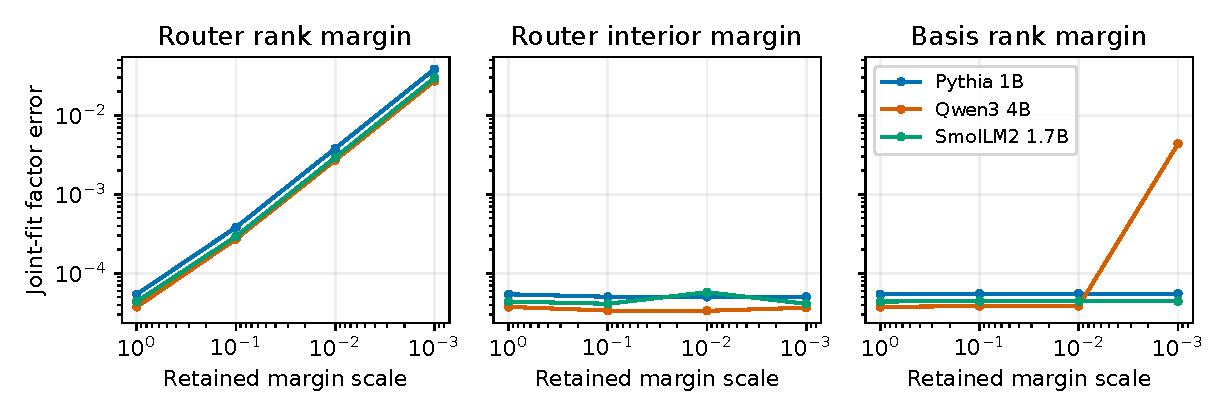
\includegraphics[width=\linewidth]{figures/llm_conditioning.pdf}
\caption{Secondary stress at observation noise $10^{-4}$.
Shrinking router rank amplifies error from roughly $4$--$5\times10^{-5}$
 to $0.027$--$0.038$. The other tested paths do not show comparable
 monotone growth; the absence of failure on a selected path does not
 remove the theorem's nondegeneracy assumptions.}
\label{fig:llm-conditioning}
\end{figure}

\subsection{Matched structural decisions and repeat controls}

The predeclared decision units are Pythia1B, Qwen3-4B and SmolLM2-1.7B,
 each at seeds0/1/2. Every action uses four nonempty equal-sized groups.
The native and recovered router actions maximize balanced assignment
 scores; the effective-parameter control uses balanced $k$-means with
 deterministic farthest-point initialization and50 iterations; the random
 control uses a fixed seeded balanced partition. Recovered actions use
 general-text $q=4$ joint fits at noise $10^{-4}$ and $10^{-2}$.
Every hard group receives the mean of the same canonical FP32 effective
 tensors, followed by64 updates of only the four bases with fresh AdamW
 states, rate $10^{-4}$, zero decay, the same batch indices and clipping.
All 45 actions complete. Rejected recovery would retain the native action;
 all 18 recovered decision inputs are accepted by the combined policy.

\begin{table}[t]
\centering\small
\caption{Post-recovery NLL minus native-router partition, averaged over three seeds. All actions use four balanced groups, a common effective-tensor refit and 64 matched updates. Both recovered and effective-clustering partitions equal the native partition at all nine checkpoints. Small Pythia discrepancies under equivalent partitions are numerical execution variation, not structural improvements. Per-seed values and immediate losses are retained in the released CSV.}
\label{tab:llm-decisions}
\begin{tabular}{llrrr}
\toprule
Model & Action & General & Code & Math\\
\midrule
Pythia 1B & Effective clustering & -0.0004 & -0.0005 & -0.0001\\
Pythia 1B & Random balanced & +0.0629 & -0.0196 & -0.0291\\
Pythia 1B & Recovered, $10^{-4}$ & -0.0004 & -0.0005 & -0.0002\\
Pythia 1B & Recovered, $10^{-2}$ & +0.0001 & -0.0007 & -0.0003\\
Qwen3 4B & Effective clustering & +0.0000 & +0.0000 & +0.0000\\
Qwen3 4B & Random balanced & +0.0801 & +0.0096 & +0.0010\\
Qwen3 4B & Recovered, $10^{-4}$ & +0.0000 & +0.0000 & +0.0000\\
Qwen3 4B & Recovered, $10^{-2}$ & +0.0000 & +0.0000 & +0.0000\\
SmolLM2 1.7B & Effective clustering & +0.0000 & +0.0000 & +0.0000\\
SmolLM2 1.7B & Random balanced & +0.1050 & -0.0041 & -0.0238\\
SmolLM2 1.7B & Recovered, $10^{-4}$ & +0.0000 & +0.0000 & +0.0000\\
SmolLM2 1.7B & Recovered, $10^{-2}$ & +0.0000 & +0.0000 & +0.0000\\
\bottomrule
\end{tabular}
\end{table}


All recovered and effective-clustering partitions have zero co-membership
 difference from the native partition. General-text random-minus-native
 post-recovery NLL is $0.0383$--$0.1098$ across the nine checkpoints;
 held-out code and math differences have mixed signs. This establishes no
 advantage over the effective-parameter control. Equivalent partitions on
Pythia exhibit small numerical NLL differences under the original BF16
 execution. A labeled post hoc diagnostic repeats the \emph{identical}
 native action three times per Pythia1B seed with identical tensors,
 labels, batches and optimizer settings. The largest within-seed/domain
 NLL range is $0.00152$, confirming execution variation on the scale of
 these differences. We do not interpret them as structural improvements.
There is no measured compression speedup: the pretrained backbone remains
 stored and executed in full.

\subsection{Compute, replay and artifact scope}

\begin{table}[t]
\centering\small
\caption{Per-checkpoint costs: median over three seeds; maximum allocated GPU memory across training and observation. Training excludes loading, evaluation and gradient collection; observation covers the entire noise/query sweep; recovery is single-thread CPU time elapsed for all three estimators. Timings are local measurements under concurrent jobs.}
\label{tab:llm-cost}
\begin{tabular}{lrrrrrr}
\toprule
Model & Adapter (M) & Train (s) & Observe (s) & Recover (s) & Peak (GiB)\\
\midrule
Pythia 160M & 0.197 & 3.2 & 14.9 & 10.4 & 0.75\\
Pythia 1B & 0.524 & 5.8 & 35.6 & 9.7 & 2.65\\
Pythia 2.8B & 0.655 & 11.8 & 45.3 & 34.4 & 6.68\\
Qwen3 0.6B & 0.524 & 10.4 & 36.3 & 25.3 & 2.82\\
Qwen3 1.7B & 0.524 & 12.4 & 36.1 & 26.7 & 5.26\\
Qwen3 4B & 1.049 & 20.0 & 72.4 & 43.3 & 10.95\\
Qwen3 8B & 1.049 & 34.3 & 72.4 & 43.3 & 19.08\\
SmolLM2 360M & 0.246 & 9.9 & 18.9 & 36.0 & 1.50\\
SmolLM2 1.7B & 0.524 & 9.4 & 35.8 & 19.6 & 4.49\\
\bottomrule
\end{tabular}
\end{table}


The local machine has eight RTX5090 GPUs with about32GiB each. Model
 training uses a dedicated environment with Transformers4.57.6 and
PyTorch2.7.0a0 (NVIDIA build); the previous project environment is retained.
The largest allocated GPU footprint is19.08GiB. Per-checkpoint timing
 includes explicit synchronization for training; total training-stage
 timing additionally includes loading, evaluation and natural-gradient
 collection. Recovery is performed on CPU, with up to12 jobs in parallel.
The complete environment, source freeze, corpus lock, checkpoint hashes,
 observations and per-case solver records are retained.

An isolated PyTorch2.7.1 CPU environment replays 81 selected cases:
 every evaluation checkpoint, $q=4$, designed/noiseless and general-text
 natural queries at noise $10^{-4}$ and $10^{-2}$. Across243 estimator
 outputs, the largest permutation-aligned estimate difference is
$1.39\times10^{-10}$, and all acceptance decisions agree. Three additional
 full-dimensional natural-query checks compare explicit analytic residuals
 against the compressed objective for deliberately wrong candidates;
 absolute discrepancies are below $3.8\times10^{-15}$. This is independent
 arithmetic replay, not independent pretrained-model training or external
 peer review. The source package contains the manuscript; the research
 artifact separately contains observations, checkpoints, protocols and
 commands. Upstream model weights and raw gradient caches are not bundled
 with the manuscript. Scripts regenerate them from pinned inputs.

\section{Earlier synthetic and byte-language-model illustrations}
\label{app:earlier-illustrations}

This appendix preserves the earlier studies, separately from the pretrained-model study in Section~\ref{sec:experiments}. The theory is the main evidence for the global statements. These earlier experiments
check the response formula, illustrate finite reconstruction, and expose
precision and conditioning limits. They use the exact-product design of
Corollary~\ref{cor:response_tomography} or rank-checked natural/Gaussian
probes, \emph{not} the repeated-complement design of
Corollary~\ref{cor:finite-noisy-main}. Thus they do not empirically evaluate
its whole-feasible-set diameter bound. All numerical tables come from
validated result records; protocols, negative results, source hashes, and
replay limitations are retained in
Appendices~\ref{sec:benchmark}--\ref{app:trusted-experiments}.

\paragraph{Independent full-dimensional response measurements.}
Three soft-router byte-LM checkpoints have $L=12$, $K=4$, and $D=787{,}712$.
We measure responses by reverse-mode differentiation of a linear effective
loss followed by a forward-mode JVP of the packed factor-to-product map.
The observation code does not call Equation~\ref{eq:response_blocks}.
For each native, permutation, and fixed non-permutation chart, four designed
probes reconstruct the response and two unseen Gaussian probes test its
predictions. Table~\ref{tab:autograd-tomography} shows numerical agreement
with the formula, successful held-out prediction, and separation of the
fixed alternative. This finite check does not prove separation of every
possible alternative; that quantifier is supplied by the theorem.

% Generated by experiments/summarize_autograd_tomography.py.
\begin{table}[H]
\centering\small
\caption{Full-dimensional autodiff response audit. Errors are relative Frobenius norms. Formula and held-out columns take the maximum over native, permutation, and non-permutation charts; each chart uses four designed and two unseen probes.}
\label{tab:autograd-tomography}
\begin{tabular}{@{}crrrr@{}}
\toprule
Seed & Formula error & Held-out error & Permutation gap & Non-perm. gap \\
\midrule
0 & 3.52e-16 & 4.68e-14 & 9.73e-17 & 0.9734 \\
1 & 3.37e-16 & 5.07e-14 & 1.05e-16 & 0.9731 \\
2 & 3.71e-16 & 4.12e-14 & 1.11e-16 & 0.9735 \\
\bottomrule
\end{tabular}
\end{table}


\paragraph{Natural directions and finite precision.}
Actual byte-LM cross-entropy gradients with respect to independent effective
layer weights supply 16 directions per checkpoint. Controlled autodiff
responses are measured at a fixed checkpoint; the first $q\in\{1,4,8,12\}$
directions fit the structural estimator and the last four test prediction.
With the exact product row space, four directions meet the sufficient
reconstruction ranks at all six checkpoints in
Table~\ref{tab:natural-gradients}. Factor errors use permutation alignment
only for evaluation. One direction has insufficient local rank and gives
errors $0.258$--$1.34$ at the three longer-trained checkpoints.

% Keep the generated second table after the first without changing its source.
\begingroup
\let\originaltable\table
\renewcommand{\table}[1][]{\originaltable[H]}
\begin{table}[t]
\centering\small
\caption{Four natural task-gradient probes with known response structure. Original and new checkpoints use the separately registered 1,500- and 6,000-step configurations. Recovery error is the combined relative factor error after evaluation-only permutation alignment. These are FP64 fixed-checkpoint measurements, not observed training trajectories.}
\label{tab:natural-gradients}
\begin{tabular}{llrr}
\toprule
Configuration & Seed & Max. held-out response error & Factor error \\
\midrule
Original & 0 & $9.57\times10^{-14}$ & $3.02\times10^{-8}$ \\
Original & 1 & $8.22\times10^{-14}$ & $5.37\times10^{-9}$ \\
Original & 2 & $8.63\times10^{-14}$ & $1.36\times10^{-8}$ \\
New & 10 & $9.39\times10^{-14}$ & $2.31\times10^{-8}$ \\
New & 11 & $6.45\times10^{-14}$ & $1.35\times10^{-8}$ \\
New & 12 & $9.95\times10^{-14}$ & $1.48\times10^{-8}$ \\
\bottomrule
\end{tabular}
\end{table}

\endgroup

Finite Euclidean steps reveal an arithmetic limit. At step size $10^{-5}$,
the longer-trained checkpoints have FP64 response errors
$3.3\times10^{-8}$--$5.2\times10^{-8}$, but FP32 subtraction errors
$0.0208$--$0.0260$ and BF16 errors about one. These tests cast factors and
arithmetic to the stated precision; they do not test mixed-precision
training with FP32 master weights. The step-size sweep is in
Appendix~\ref{app:enhancement-experiments}.

\paragraph{Noisy recovery does not supply an automatic trust certificate.}
A separate frozen development/calibration/evaluation protocol compares
spectral recovery, simplex projection with a basis refit, and three-start
constrained joint least squares. Both the product and measured responses
receive relative noise up to $10^{-2}$; the estimated product subspace is
recomputed. On 1,920 held-out synthetic variants across 40 seeds, joint
fitting reduces the median factor error from $3.34\times10^{-3}$ for
projected spectral recovery to $1.01\times10^{-4}$, and errors above $0.10$
from 566 to 227. All 48 variants at four fresh byte-LM checkpoints have
joint-fit errors below $0.0107$.

Failures remain substantial: the largest joint-fit error is $10.54$, and a
combined diagnostic falsely accepts an error of $0.82$. Its accepted-bad
fraction is $92/1782=5.16\%$, with seed-cluster bootstrap interval
$[4.50\%,5.79\%]$; residual-only rejection yields $68/1757=3.87\%$.
The combined score therefore does not establish superiority, and its point
estimate exceeds the $5\%$ calibration target. The candidate-local checks
also do not exclude distant solutions or establish truth membership in the
fitted subspace. Appendix~\ref{app:trusted-experiments} retains all methods,
tail errors, failed solver statuses, and independent CPU replay differences.
None of these diagnostics is the global certificate above.

\paragraph{Auxiliary structural decisions.}
Identifying coordinates under an optimizer does not make actions derived
from them product invariant. In a documented reimplementation of ASLoRA's
first RoBERTa/MRPC merge rule, a fixed grid changes the primary action in
$11/30$ seed--gauge instances. Only the selected layer indices are carried
back to a common canonical model; validation-loss differences have both
signs. A separate controlled byte-LM partition audit finds changes at all
three longer-trained checkpoints, but matched recovery training greatly
reduces the performance gaps. These are bounded decision witnesses, not
applications of the softmax theorem to LoRA, universal harm claims, or
full-training regret evaluations. Detailed results, failed signed-local
searches, and the earlier initialization-dominated experiment remain in
Appendices~\ref{app:detailed-results} and~\ref{app:enhancement-experiments}.

\section{Detailed audit protocols and historical settings}
\label{sec:benchmark}

This appendix preserves the protocols for the original response and
decision audits. The current numerical overview is in
Section~\ref{sec:experiments}; the later controlled partition experiments and
noisy-recovery studies have separate protocols in
Appendices~\ref{app:enhancement-experiments} and~\ref{app:trusted-experiments}.
They use different training configurations and must not be pooled as one
replication rate.

\subsection{Frozen-checkpoint response audit}

We first audit the distinguishing observation used by the new theorem: the
instantaneous Euclidean response of the \emph{current} softmax-router chart.
At each of three independently trained soft-router byte-LM checkpoints, we
verify the theorem's assumptions and exact gauge construction.  On a
predeclared $4\times32$ extraction we check
Equation~\ref{eq:response_blocks} against autograd and finite differences; on
the full $12\times787{,}712$ factor model we evaluate eight seeded Gaussian
directions plus a permutation control.  Separately, the $K=4$ interventions of
Corollary~\ref{cor:response_tomography} reconstruct the structured response.
Their full-dimensional outputs are analytic equation evaluations---not four
full-model JVP calls---with the extraction supplying the implementation check.
The Gaussian test is fixed-alternative; tomography assumes exact common
product, rank/dimension conditions, and this response family.  Neither is an
AdamW-trajectory or historical-graph claim.

An additive full-dimensional audit replaces the analytic observations with
reverse-mode factor gradients followed by forward-mode JVPs of the packed
effective-parameter map. It retains the same three checkpoints and fixed
gauge, uses two unseen response directions per chart to test reconstruction,
and records a five-level fixed-norm observation-noise sensitivity grid.
Its prospective local protocol, source bindings, and numerical gates are
released separately from the original audit; no retraining is involved.

\subsection{ASLoRA first-merge decision audit}
\label{sec:aslora-protocol}

This auxiliary decision experiment audits a documented reimplementation of the
accessible ASLoRA-v2 first-merge rule~\citep{hu2024aslorav2}.  We train
rank-eight, $\alpha=16$ adapters on
RoBERTa-base/MRPC to the first scheduled merge opportunity, optimizer step
$560$.  Query and value select separate pairs; a joint pair is sensitivity
analysis.  Because the source leaves adjacent-versus-all-pairs candidates
ambiguous, we report both.  A frozen bank contains identity, orthogonal,
diagonal, and dense gauges.  Each float64 gauge selects only a layer-index
action by running-$B$ distance; we then apply the same temporary directed tie
in the unchanged canonical model and evaluate the full validation split.

The selection proxy and the executed action are different estimands.  Writing
$c=\alpha/r$, the common change of rank coordinates
$B_{i,Q}=B_iQ$, $A_Q=Q^{-1}A$ leaves
$cB_{i,Q}A_Q=cB_iA$ fixed, but scores a candidate
$p=(\ell\leftarrow u)$ by the order-equivalent squared score
\begin{equation}
 s_p(Q)=\|({\bar B}_\ell-{\bar B}_u)Q\|_F^2.
 \label{eq:aslora_selection_score}
\end{equation}
Executing that index action instead replaces the \emph{current} $B_\ell^t$
by $B_u^t$; its immediate weight perturbation is
$c(B_u^t-B_\ell^t)A$, and its lower-layer local RMS disturbance is
$\{\mathbb E\|c(B_u^t-B_\ell^t)Ax_\ell\|_2^2\}^{1/2}$.  Without assumptions
linking historical averages, current factors, and the lower-layer input
moment, the running score is not guaranteed to estimate action cost.

Three comparisons separate coordinate dependence from decision quality:
current effective-update Frobenius distance is gauge invariant and uses only
the prevalidation snapshot; current local-activation RMS is gauge invariant
but post-hoc and label-free; validation loss is a labeled oracle never used for
selection.  We exhaust query-only, value-only, joint-same-pair, and selected
composite actions, not their full Cartesian product.  Product invariance,
restoration, and canonical-action checks gate the run; passing live-float32
re-execution remains a numerical diagnostic, not the causal estimand.

\subsection{Historical byte-LM same-budget partition-fold search}

The original three-checkpoint experiment asked whether a controlled
downstream consequence found at one checkpoint replicated.  At each of the same three byte-LM
checkpoints, a
predeclared finite router-only search seeks a positive-stochastic gauge that
changes the argmax partition at the same four-group budget.  Both partitions
are refit from the same effective tensors and compared on paired held-out
batches; literal factor hardening is only a confounded diagnostic.  Fixed-budget
failures remain negative results, not proofs of non-existence, so one successful
checkpoint establishes possibility rather than prevalence.  All three routers
meet the protocol's initialization-dominated flag.  Signed-local and same-sorted-group-size searches were unexecuted
post-run amendments to this original protocol. They were subsequently
executed at three fresh, more extensively trained checkpoints under the
separate protocol in Appendix~\ref{app:enhancement-experiments}.

\section{Detailed numerical results and auxiliary decisions}
\label{app:detailed-results}

The audit and extension tables are generated from validated summary JSON artifacts,
including negative seeds and failed searches; exact paths and hashes are
recorded in Appendix~\ref{app:experimental-details}.

\subsection{A non-permutation chart is visible in optimizer response}

% Auto-generated by experiments/generate_paper_audit_tables.py; do not edit.
% Source: results/response_summary.json
% Source SHA256: fd3f8ade6b43e6830e5a5c6bdc188509b77da844c4fa977c5d25e5af1e3d3224
\providecommand{\ResponseProbeDetected}{24}
\providecommand{\ResponseProbeExpected}{24}
\providecommand{\ResponseEffectiveMax}{\ensuremath{1.70\!\times\!10^{-16}}}
\providecommand{\ResponseFormulaMax}{\ensuremath{9.57\!\times\!10^{-13}}}
\providecommand{\ResponsePermutationMax}{\ensuremath{8.82\!\times\!10^{-17}}}
\providecommand{\ResponseMedianMin}{0.5045}
\providecommand{\ResponseMedianMax}{0.5058}
\begin{table}[H]
\centering
\scriptsize
\caption{Frozen-checkpoint response audit.  The effective-product column checks the fixed non-permutation gauge; $\Delta\mathcal R$ compares Euclidean instantaneous response operators on fixed Gaussian effective-gradient probes.  The permutation column is the label-swap control.}
\label{tab:response-audit}
\resizebox{\linewidth}{!}{%
\begin{tabular}{crrrrrrr}
\toprule
Seed & Effective product rel. error & $\min A$ & $\sigma_{\min}(A)$ & $\sigma_{\min}(B)$ & Perm. max rel. $\Delta\mathcal R$ & Nonperm. median rel. $\Delta\mathcal R$ & Detected probes \\
\midrule
0 & $1.58\!\times\!10^{-16}$ & $2.88\!\times\!10^{-4}$ & 1.7291 & 27.445 & $8.82\!\times\!10^{-17}$ & 0.5045 & 8/8 \\
1 & $1.70\!\times\!10^{-16}$ & $2.72\!\times\!10^{-4}$ & 1.7291 & 27.339 & $8.82\!\times\!10^{-17}$ & 0.5051 & 8/8 \\
2 & $1.63\!\times\!10^{-16}$ & $2.61\!\times\!10^{-4}$ & 1.7290 & 27.371 & $8.82\!\times\!10^{-17}$ & 0.5058 & 8/8 \\
\bottomrule
\end{tabular}%
}
\end{table}


Table~\ref{tab:response-audit} checks the response formula and separates
a fixed alternative at frozen checkpoints under
Theorem~\ref{thm:response_stabilizer}'s assumptions.  All stated rank conditions hold, the
non-permutation reparameterization preserves the effective model to at most
\ResponseEffectiveMax{} relative error.  On the declared $4\times32$
extraction, the analytic response agrees with autograd within numerical
precision, and the worst finite-difference error across native and transformed
charts is \ResponseFormulaMax{}.  The maximum permutation-control discrepancy
is \ResponsePermutationMax{} after rounding, whereas all
\ResponseProbeDetected{}/\ResponseProbeExpected{} checkpoint--probe
evaluations detect a change (eight per checkpoint, with overlapping seed
windows and 10 unique Gaussian draws; per-seed medians
$[\ResponseMedianMin{},\ResponseMedianMax{}]$).
The separate structured audit reduces the all-gradient quantifier to
\ResponseTomographyProbeCount{} designed analytic response evaluations, which
reconstruct all response components with worst relative error
\ResponseTomographyReconstructionMax{}; the
permutation control stays below \ResponseTomographyPermutationMax{}; the
minimum across seeds of each seed's maximum fixed non-permutation difference
over the four designed probes is \ResponseTomographyNonpermutationMin{} after
rounding.  This does not say that every individual probe reaches that value.
These are analytic evaluations of
Equation~\ref{eq:response_blocks}, validated on the extraction, not four
full-model JVP calls.  The eight Gaussian probes remain a fixed-alternative
test; the designed certificate assumes exact common product and the stated
response family.  Neither audit describes AdamW or a historical graph.

\paragraph{Independent full-dimensional response measurements.}
A subsequent audit obtains the responses by differentiating the complete
packed map $(Z,B)\mapsto\operatorname{softmax}(Z/\tau)B$ at all three
released checkpoints. Reverse-mode differentiation of a linear probe loss
gives the factor gradients; a forward-mode JVP then measures the induced
effective-parameter response. The observation code does not call the analytic
response formula. Each native, permutation, and fixed non-permutation chart
uses four designed probes and two unseen Gaussian probes.
Table~\ref{tab:autograd-tomography} reports formula agreement and prediction of
the unseen responses from the reconstructed operator. The maximum relative
formula discrepancy is $3.71\times10^{-16}$, and the maximum held-out response
error is $5.08\times10^{-14}$. A five-level observation-noise grid from zero
to $10^{-4}$ relative Frobenius norm satisfies the deterministic component
error bounds, with recorded floating-point slack. These measurements concern
the full shared-parameter map, not an end-to-end language-model loss or an
AdamW step; operator reconstruction does not itself implement noisy factor
recovery. The additive records preserve the original analytic audit.



\paragraph{Exploratory reconstruction of the factors.}
The construction in Appendix~\ref{app:response_tomography} recovers factors
from the effective product and measured components, without supplying the
original factors to the reconstruction. We test it on the native charts of
the same three checkpoints, using fresh autodiff observations and one fixed
Gaussian weight vector for joint diagonalization. Table~\ref{tab:factor-recovery}
reports the errors after a common permutation chosen only for evaluation.
The noiseless combined relative errors are below $3.7\times10^{-9}$.
All five noise levels complete without a rank or eigengap failure, but the
unprojected noisy estimates need not have exact unit row sums. These are
three checkpoint diagnostics with exact effective products, not independent
training replications, adversarial-noise tests, or a general stability result
for the PSD-clipped recovery algorithm.

% Generated by experiments/summarize_factor_recovery.py.
\begin{table}[H]
\centering\small
\caption{Exploratory factor recovery from full-dimensional autodiff observations. Orbit error combines relative router and basis errors after one common permutation. Noisy rows use relative observation noise $10^{-4}$ and no simplex projection.}
\label{tab:factor-recovery}
\begin{tabular}{@{}crrr@{}}
\toprule
Seed & Noiseless orbit error & Noisy orbit error & Noisy row-sum error \\
\midrule
0 & 3.66e-09 & 1.81e-05 & 6.06e-05 \\
1 & 3.23e-09 & 1.61e-05 & 6.68e-05 \\
2 & 3.28e-09 & 1.59e-05 & 5.99e-05 \\
\bottomrule
\end{tabular}
\end{table}


\subsection{Gauge-equivalent ASLoRA states change the first merge decision}
\label{sec:aslora-results}

% Auto-generated by experiments/generate_paper_audit_tables.py; do not edit.
% Source: results/aslora_summary.json
% Source SHA256: 1be80d31ca4208c414698c3b5fbd45bfb9d51835aa8f16f8cb43bab082840c41
\providecommand{\ASLORAAdjacentPrimaryChanges}{11}
\providecommand{\ASLORAAllPrimaryChanges}{14}
\providecommand{\ASLORATotalGaugeInstances}{30}
\providecommand{\ASLORAGaugesPerSeed}{10}
\begin{table}[H]
\centering
\small
\setlength{\tabcolsep}{3pt}
\caption{ASLoRA first-merge decision audit over \ASLORAGaugesPerSeed{} gauges per seed.  Changes are relative to the identity-gauge raw-running-$B$ action.  The loss interval is the canonical validation difference (selected action minus identity action), not a gauged float32 re-execution; accuracy and F1 intervals are in Appendix Table~\ref{tab:aslora-metric-details}.  The chain column requires a changed action with a nonzero validation consequence in every seed.}
\label{tab:aslora-chain}
\begin{tabular}{@{}llcrrcc@{}}
\toprule
Candidates & Scope & By seed & Changed & Seeds & $\Delta$ loss & Chain \\
\midrule
Adjacent & per-proj. & $(2,6,3)$ & 11/30 & 3/3 & $[-0.0531,+0.0089]$ & yes \\
Adjacent & joint pair & $(0,5,0)$ & 5/30 & 1/3 & $[+0.0000,+0.0077]$ & no \\
All pairs & per-proj. & $(4,7,3)$ & 14/30 & 3/3 & $[-0.0531,+0.0027]$ & yes \\
All pairs & joint pair & $(0,0,0)$ & 0/30 & 0/3 & $[+0.0000,+0.0000]$ & no \\
\bottomrule
\end{tabular}
\end{table}


The primary per-projection chain replicates under both readings of the source's
candidate set.  Among \ASLORATotalGaugeInstances{} predeclared gauge instances,
the raw-running-$B$ action changes in
\ASLORAAdjacentPrimaryChanges{} instances for adjacent candidates and
\ASLORAAllPrimaryChanges{} instances for all pairs.  Every seed has at least
one changed action with a nonzero canonical validation consequence under both
candidate readings.  The signs in Table~\ref{tab:aslora-chain} go in both
directions: the experiment demonstrates representation-dependent decisions,
not that every gauge-induced change is harmful or that the identity action is
optimal.  The joint-same-pair sensitivity does not replicate (one seed for
adjacent candidates and none for all pairs), and Appendix
Table~\ref{tab:aslora-baselines} shows that neither gauge-invariant rule
uniformly improves on raw running \(B\) across all seeds under both candidate
readings.  The causal contrast uses a
float64-equivalent snapshot only to select layer indices, then executes the
same temporary tie in the unchanged canonical model; factorized-float32
re-execution is a passing secondary diagnostic.  Thus the complete chain is
concrete but local to one first merge, method, task, and fixed gauge grid.

\subsection{Prospective controls: learned routers and recovery training}
\label{sec:enhanced-decisions}

The historical witness in Appendix~\ref{app:historical-fold-witness}
motivates a separately registered extension;
it does not supply its outcomes. We train three fresh width-128, twelve-layer,
four-basis byte LMs for a fixed 6,000 steps with random router initialization
and a separate router learning rate. Router L1 movement is $0.593$--$0.729$;
all three models pass the unigram-improvement and router-movement gates.
Both gauge families receive 5,000 router-only trials, now requiring the same
sorted group-size multiset as the native partition. Positive-stochastic
search finds a first valid candidate in every seed; signed-local search fails
in all three. Failures are retained and never replaced by larger searches.

\begin{table}[t]
\centering\small
\caption{Prospective equal-size folding audit. Signed BPB differences are gauge-selected minus native-selected folds after matched recovery updates. Each row is one independent training seed. Positive-stochastic search succeeds in 3/3 seeds; signed-local search fails in 3/3, each with 5,000 router-only candidates.}
\label{tab:enhanced-decisions}
\begin{tabular}{rrrrr}
\toprule
Seed & Router movement & $\Delta_0$ & $\Delta_{100}$ & $\Delta_{500}$ \\
\midrule
10 & 0.593 & -0.00112 & +0.00224 & +0.00009 \\
11 & 0.720 & +0.87112 & +0.03574 & +0.01823 \\
12 & 0.729 & +0.14873 & +0.00580 & +0.00343 \\
\bottomrule
\end{tabular}
\end{table}


Every fold uses the same native effective tensors. Hard routes remain fixed
while all remaining parameters receive identical minibatches, optimizer
initialization, update counts, and learning rates. Table~\ref{tab:enhanced-decisions}
shows substantial immediate differences in two seeds, but much smaller
differences after 500 recovery updates. Conditional paired 95\% bootstrap
intervals at that stage are $[-0.00094,0.00112]$, $[0.01654,0.01989]$, and
$[0.00244,0.00437]$ BPB, respectively; they describe the fixed evaluation
blocks, not uncertainty over training populations. The same-size
effective-parameter local-search baseline selects the native partition in
two seeds and performs slightly worse after recovery in the third.
Thus removing the earlier initialization and size confounds strengthens the
decision-sensitivity evidence, without establishing persistent large harm or
general superiority of an invariant rule. This is one architecture and corpus,
with a fixed training budget rather than a convergence certificate.

\subsection{Natural task gradients and finite arithmetic}
\label{sec:natural-gradients}

We differentiate actual byte-LM cross-entropy with respect to independent
layer-effective weights, holding other parameters fixed. A separate forward
and chain-rule check agrees with the original model. At each of the three
original and three new checkpoints, 16 fixed training minibatches supply
natural directions. Controlled reverse/forward autodiff measures the response;
the first $q\in\{1,4,8,12\}$ directions fit the estimator, and the last four
test prediction. The estimator uses the exact product row space and known
response structure, not the true factors.



At $q=4$, all six checkpoints meet the rank conditions of
Proposition~\ref{prop:natural-probes}. The largest held-out response error is
below $10^{-13}$ and the factor error below $3.1\times10^{-8}$.
This is stronger than separation of a single alternative chart, but remains
conditional on the known Euclidean response family and precise measurements.
A single direction has insufficient local rank; at the new checkpoints its
factor errors range from $0.258$ to $1.34$. Generic linear prediction from the
observed gradient span also differs from the structural estimator. These
directions are measurements at fixed checkpoints, not observations of an
uncontrolled training trajectory.

Explicit finite Euclidean steps expose a numerical boundary. At step size
$10^{-5}$, the new checkpoints' FP64 response errors are
$3.3\times10^{-8}$--$5.2\times10^{-8}$, whereas FP32 subtraction errors are
$0.0208$--$0.0260$ and BF16 errors are about one.
Here factors and arithmetic are cast to the stated precision; this is not a
test of BF16 training with FP32 master weights. Appendix
Figure~\ref{fig:enhancement-precision} reports the step-size tradeoff and the
separate joint-noise conditioning diagnostic.

\subsection{Noisy recovery and the limits of observable rejection}
\label{sec:trusted-recovery}

We fix a prospective development/calibration/evaluation split before
measuring the final outcomes. Forty held-out synthetic seeds each contribute
48 correlated noise/probe/regime variants; four freshly trained byte-LM
checkpoints each contribute 12. Both product and autodiff response
observations receive relative noise from zero to $10^{-2}$, and the rank-$K$
product row subspace is re-estimated from the noisy product.
Three fixed methods use the same observations: spectral recovery,
simplex projection with a basis refit, and three-start constrained joint
least squares. The estimator never receives the true factors.
Appendix~\ref{app:trusted-experiments} gives splits, budgets, calibration,
and all diagnostic comparators.

\begin{table}[t]
\centering
\small
\caption{Frozen held-out noisy recovery. Each synthetic instance contributes 48 correlated variants; each language checkpoint contributes 12. Acceptance uses the calibrated empirical score. Bad means factor error $>0.10$; good means $\le0.05$. Local passes concern only a numerical restricted-subspace component.}
\label{tab:trusted-recovery}
\begin{tabular}{llrrrrr}
\toprule
Domain & Method & Median error & Bad/total & Accept & Bad/accept & Local \\
\midrule
Synthetic & Spectral & 0.0041 & 564/1920 & 196 & 0/196 & 0 \\
Synthetic & Projected & 0.0033 & 566/1920 & 1396 & 56/1396 & 0 \\
Synthetic & Joint fit & 0.0001 & 227/1920 & 1782 & 92/1782 & 140 \\
Byte-LM & Spectral & 0.00017 & 1/48 & 0 & -- & 0 \\
Byte-LM & Projected & 0.0002 & 1/48 & 48 & 1/48 & 0 \\
Byte-LM & Joint fit & 3.3e-05 & 0/48 & 48 & 0/48 & 2 \\
\bottomrule
\end{tabular}
\end{table}


Joint fitting reduces the synthetic median factor error from
$3.34\times10^{-3}$ for projected spectral recovery to $1.01\times10^{-4}$,
and the number of errors above $0.10$ from $566$ to $227$ out of $1920$.
At the four byte-LM checkpoints, all 48 joint-fit errors are below $0.0107$,
including the $1\%$ observation-noise cases. These are controlled Euclidean
measurements at checkpoints, not noisy AdamW trajectory observations.

The more demanding question is whether an observable diagnostic can tell
when to trust a result. With its threshold fixed on separate calibration
data, the combined residual/conditioning/subspace/multi-start score accepts
$1782/1920$ synthetic outputs, including 92 bad outputs. Its $5.16\%$
accepted-bad fraction has a seed-cluster bootstrap interval of
$[4.50\%,5.79\%]$ and has a point estimate above the $5\%$ calibration target;
the interval includes that target.
Residual-only rejection accepts $1757/1920$ with $68/1757=3.87\%$ bad.
Thus, the combined score does not establish superiority.
The full evaluation retains a joint-fit error of $10.54$, and a falsely
accepted error of $0.82$. These failures prevent a general reliability claim.

The explicit local separation bound in
Proposition~\ref{prop:trusted-local} addresses a different question.
Only $140/1920$ synthetic and $2/48$ language outputs pass its numerical
local-component conditions. These passes neither establish truth membership
in the restricted subspace nor rule out distant solutions.

\section{Experimental details}
\label{app:experimental-details}

\subsection{Original audit inventory}

Table~\ref{tab:primary-audit-inventory} records the original audit units.  The three response checkpoints and three byte-LM decision checkpoints
are paired by training seed.  The ASLoRA runs are a separate RoBERTa-base/MRPC
experiment.

All numerical entries in the three original audit tables are generated directly from
\texttt{results/response\_summary.json},
\texttt{results/aslora\_summary.json}, and
\texttt{results/router\_decisions\_summary.json} by
\texttt{experiments/generate\_paper\_audit\_tables.py}.  Each generated file
records the SHA256 of its source summary, retaining negative seeds and failed
searches in the reported aggregates; the same script emits the appendix metric
and search-detail tables.  The additive tomography numbers are
generated separately from
\texttt{results/response\_tomography\_summary.json} by
\texttt{experiments/generate\_response\_tomography\_latex.py}; this leaves the
source-attested older response table unchanged.
The subsequent full-dimensional autodiff and factor-recovery tables are
generated by their separate summarizers from
\texttt{results/autograd\_tomography/} and
\texttt{results/factor\_recovery/}. Both validate generation-source and
checkpoint hashes. They reuse the same three checkpoints and therefore do
not increase the number of independent training seeds.

\begin{table}[H]
\centering
\small
\caption{Original primary audit inventory. Each audit has three seeds;
counts include failed searches and controls. Additive audits reuse the
response checkpoints, as detailed below.}
\label{tab:primary-audit-inventory}
\begin{tabular}{@{}p{.20\linewidth}p{.39\linewidth}p{.32\linewidth}@{}}
\toprule
Audit & Per-seed protocol & Required checks \\
\midrule
Optimizer response & 8 Gaussian and 4 designed probes; fixed non-permutation and permutation control & Rank, formula, exact-gauge product, reconstruction \\
ASLoRA first merge & 10 gauges; adjacent/all pairs and per-projection/joint actions & Coverage, canonical action, restoration \\
Byte-LM partition fold & 5,000 trials; four-group, same-effective refits & Fixed search and paired evaluation \\
\bottomrule
\end{tabular}
\end{table}

The response audit uses a fixed gauge strength of $0.35$, unit Euclidean
learning rates for both parameter blocks, and probe seeds determined before
evaluation.  Each result records its checkpoint and source hashes.  The best
finite-difference scale on a predeclared four-row, 32-coordinate checkpoint
extraction is selected only to validate the closed-form response; the eight
fixed Gaussian directions on the full $12\times787{,}712$ packed model provide
the separate non-permutation detection test.  The additive four-probe audit
constructs the Corollary~\ref{cor:response_tomography} design from \(\Theta\)
and reconstructs the response components.  Its full-dimensional responses are
evaluations of the already checked analytic formula, not four additional
full-model autograd/JVP calls.  Its version-2 artifacts separately record the
reference rank/dimension gate, the floating-point product residual, and exact
common-product validity from the explicit invertible-gauge construction.

The subsequent autodiff audit instead differentiates the packed factor map.
For each checkpoint it measures four designed and two unseen responses in
each of three charts: native, permutation, and a fixed non-permutation gauge.
Its five-level observation-noise diagnostic uses the native chart. The
factor-recovery pilot makes four fresh native-chart measurements, reuses one
fixed diagonalization weight seed across checkpoints, and reports all five
noise levels without selecting a favorable weight vector. True factors enter
the observation oracle and post-reconstruction error calculation, but not the
reconstruction routine. Neither experiment differentiates the language-model
task loss or simulates an AdamW trajectory.

The ASLoRA protocol follows the paper's defined configuration: 30 epochs,
effective batch size 16, rank eight, $\alpha=16$, $T_s=320$, and merge interval
240.  Appendix Table~5 of the source additionally records an update ratio
$\lambda=0.5$, but the accessible method text and Algorithm~1 define no
operation involving that quantity.  We record $\lambda$ in provenance as
\texttt{update\_ratio\_record\_only} and deliberately do not invent an
implementation for it.  With the one-indexed rule $t>T_s$ and
$(t-T_s)\bmod 240=0$, the first audit point is $t=560$.  Running $B$ is observed
after every optimizer update.  The three
artifacts contain 204, 208, and 200 canonical action evaluations, respectively:
all 66 query-only, 66 value-only, and 66 joint-same-pair actions plus every
additional composite selected by a declared baseline or gauge.  There are no
missing or undeclared candidates.  Every temporary tie is restored, the
trainable digest and parameter identities agree before and after the audit, and
no merge is committed.

The amendment chronology in
\texttt{research/ASLORA\_EMPIRICAL\_PROTOCOL.md} records the superseded
nondeterministic \(12/30\) and \(16/30\) batch, its source hashes, the
outcome-blind deterministic protocol lock, and the canonical replacement by
the \(11/30\) and \(14/30\) results reported here.

For transparency, the ASLoRA artifacts contain two numerical paths.  The
scientific path transforms the frozen running factors in float64, chooses a
layer-index action, and evaluates that action in the canonical model.  All
canonical gates pass.  The diagnostic path re-executes the live factorized
float32 model and also passes its tolerance in all three deterministic runs.
No main-paper metric is taken from that diagnostic path.  Both
candidate interpretations are retained because Algorithm~1 and the prose in
the source differ on whether all or only adjacent layer pairs are sorted.

% Auto-generated by experiments/generate_paper_audit_tables.py; do not edit.
% Source: results/aslora_summary.json
% Source SHA256: 1be80d31ca4208c414698c3b5fbd45bfb9d51835aa8f16f8cb43bab082840c41
\begin{table}[H]
\centering
\small
\caption{Canonical validation accuracy and F1 differences for the four ASLoRA candidate/scope cells in Table~\ref{tab:aslora-chain}.  Intervals range over all 30 selected gauge actions in each cell, including unchanged selections, and are selected-action minus identity-action differences.}
\label{tab:aslora-metric-details}
\begin{tabular}{@{}llcc@{}}
\toprule
Candidates & Scope & $\Delta$ accuracy & $\Delta$ F1 \\
\midrule
Adjacent & per-projection & $[-0.0025,+0.0098]$ & $[-0.0022,+0.0057]$ \\
Adjacent & joint pair & $[-0.0049,+0.0000]$ & $[-0.0051,+0.0000]$ \\
All pairs & per-projection & $[-0.0025,+0.0098]$ & $[-0.0022,+0.0057]$ \\
All pairs & joint pair & $[+0.0000,+0.0000]$ & $[+0.0000,+0.0000]$ \\
\bottomrule
\end{tabular}
\end{table}


% Auto-generated by experiments/generate_paper_audit_tables.py; do not edit.
% Source: results/aslora_summary.json
% Source SHA256: 1be80d31ca4208c414698c3b5fbd45bfb9d51835aa8f16f8cb43bab082840c41
\begin{table}[H]
\centering
\small
\caption{Declared alternatives for the primary per-projection ASLoRA decision.  Effective-update and local-activation rules are gauge invariant.  Their cells give the selected action and canonical validation-loss difference from the identity raw-$B$ action (negative is lower; exact zero is a tie).  Across the six rows, effective has 2 negative/2 positive/2 zero differences and local activation has 2 negative/1 positive/3 zero differences; neither rule uniformly improves across all seeds under both candidate readings.  Validation minima are separate query-only and value-only enumerations; they are not a full Cartesian per-projection oracle.}
\label{tab:aslora-baselines}
\setlength{\tabcolsep}{3pt}
\begin{tabular}{ccllll}
\toprule
Seed & Candidates & \shortstack[l]{Raw running $B$} & \shortstack[l]{Current effective} & \shortstack[l]{Local activation} & \shortstack[l]{Single-target\\minima} \\
\midrule
0 & Adjacent & \shortstack[l]{$Q:0\leftarrow1$\\$V:0\leftarrow1$} & \shortstack[l]{$Q:0\leftarrow1$\\$V:10\leftarrow11$\\$\Delta L=-0.0336$} & \shortstack[l]{$Q:0\leftarrow1$\\$V:0\leftarrow1$\\$\Delta L=+0.0000$} & \shortstack[l]{$Q:6\leftarrow7$\\$V:10\leftarrow11$} \\
0 & All pairs & \shortstack[l]{$Q:0\leftarrow1$\\$V:0\leftarrow1$} & \shortstack[l]{$Q:0\leftarrow1$\\$V:1\leftarrow11$\\$\Delta L=-0.0075$} & \shortstack[l]{$Q:0\leftarrow1$\\$V:0\leftarrow11$\\$\Delta L=-0.0008$} & \shortstack[l]{$Q:6\leftarrow9$\\$V:10\leftarrow11$} \\
1 & Adjacent & \shortstack[l]{$Q:0\leftarrow1$\\$V:2\leftarrow3$} & \shortstack[l]{$Q:0\leftarrow1$\\$V:10\leftarrow11$\\$\Delta L=+0.0018$} & \shortstack[l]{$Q:0\leftarrow1$\\$V:0\leftarrow1$\\$\Delta L=+0.0001$} & \shortstack[l]{$Q:4\leftarrow5$\\$V:3\leftarrow4$} \\
1 & All pairs & \shortstack[l]{$Q:0\leftarrow2$\\$V:0\leftarrow2$} & \shortstack[l]{$Q:0\leftarrow3$\\$V:10\leftarrow11$\\$\Delta L=+0.0028$} & \shortstack[l]{$Q:0\leftarrow3$\\$V:0\leftarrow11$\\$\Delta L=-0.0005$} & \shortstack[l]{$Q:4\leftarrow11$\\$V:3\leftarrow5$} \\
2 & Adjacent & \shortstack[l]{$Q:0\leftarrow1$\\$V:0\leftarrow1$} & \shortstack[l]{$Q:0\leftarrow1$\\$V:0\leftarrow1$\\$\Delta L=+0.0000$} & \shortstack[l]{$Q:0\leftarrow1$\\$V:0\leftarrow1$\\$\Delta L=+0.0000$} & \shortstack[l]{$Q:8\leftarrow9$\\$V:8\leftarrow9$} \\
2 & All pairs & \shortstack[l]{$Q:0\leftarrow1$\\$V:0\leftarrow1$} & \shortstack[l]{$Q:0\leftarrow1$\\$V:0\leftarrow1$\\$\Delta L=+0.0000$} & \shortstack[l]{$Q:0\leftarrow1$\\$V:0\leftarrow1$\\$\Delta L=+0.0000$} & \shortstack[l]{$Q:8\leftarrow11$\\$V:8\leftarrow11$} \\
\bottomrule
\end{tabular}
\end{table}


The byte-LM search makes 5,000 predeclared positive-stochastic trials per
checkpoint and preserves a four-group action budget.  Failed searches retain
their attempted, invertible, condition-passing, simplex-passing, and
group-passing counts.  The successful contrast refits both partitions from
common effective tensors.  Literal hardening is excluded from the primary
comparison because it changes basis coordinates and the partition jointly.
All three routers satisfy the initialization-dominated flag.  Only seed 0
reaches decision evaluation: its k-means and Ward effective-tensor baselines
both have BPB $2.1753145$ and centroid SSE $5.46896\times10^{-5}$.  Seeds 1 and
2 store no folds or baseline evaluation because their searches exit first.
Signed-local and same-sorted-group-size searches were not executed in that
historical audit; they were
post-run, non-primary protocol amendments.  In particular, the observed
group-size change $3/3/3/3\to5/3/3/1$ remains a balance confound.
The reported interval resamples the 256 paired evaluation-batch differences
10,000 times. It describes evaluation variability conditional on this
checkpoint and selected contrast; it does not cover training-seed or
gauge-search uncertainty.

The protocol defines the initialization-dominated flag as mean row-wise router
$L_1$ movement from initialization strictly below $0.01$.  The three observed
movements round to $0.000313$--$0.000401$, so every checkpoint meets that
declared threshold; this flag describes training movement, not recovery of a
historical graph.

% Auto-generated by experiments/generate_paper_audit_tables.py; do not edit.
% Source: results/router_decisions_summary.json
% Source SHA256: 0e863e1db624a7f25697a7a6873e83e91f928458ba61cdfd06081e582b3e28f2
\begin{table}[H]
\centering
\small
\setlength{\tabcolsep}{4pt}
\caption{Byte-LM checkpoint and finite-search diagnostics omitted from the compact main table.  The funnel is attempted/invertible/condition-pass/simplex-pass/group-pass/partition-change.}
\label{tab:router-search-details}
\begin{tabular}{@{}crrc@{}}
\toprule
Seed & Soft BPB & Mean row router $L_1$ move & Search funnel A/I/C/S/G/P \\
\midrule
0 & 2.186 & $3.35\!\times\!10^{-4}$ & 5000/5000/4586/4586/3762/1 \\
1 & 2.188 & $3.13\!\times\!10^{-4}$ & 5000/5000/4601/4601/3790/0 \\
2 & 2.168 & $4.01\!\times\!10^{-4}$ & 5000/5000/4581/4581/3769/0 \\
\bottomrule
\end{tabular}
\end{table}

\begin{table}[H]
\centering
\small
\setlength{\tabcolsep}{3pt}
\caption{Geometry and gauge-invariant comparator details for the sole completed byte-LM witness.  The k-means and Ward folds coincide here; the unigram baseline is included only as a scale reference.}
\label{tab:router-witness-details}
\begin{tabular}{@{}crccccr@{}}
\toprule
Seed & $\kappa(Q)$ & Group sizes ref.$\to$cand. & Disagreement & k-means/Ward BPB & Centroid SSE & Unigram BPB \\
\midrule
0 & 7.93 & 3/3/3/3$\to$5/3/3/1 & 0.121 & 2.175/2.175 & $5.47\!\times\!10^{-5}$ & 4.624 \\
\bottomrule
\end{tabular}
\end{table}


\section{Secondary planted-data and probe sanity checks}
\label{app:secondary-sanity}

The experiments below were the original \TyingBench{} and \method{} suite.
They remain useful implementation and theorem sanity checks, but they do not
establish that router misinterpretation is prevalent in deployed systems, and
they are not the paper's primary empirical contribution.

\subsection{\TyingBench{} protocols}

\paragraph{Exact factorization.}
We generate $K$ orthogonal basis vectors with controlled condition number,
choose one of five depth graphs (cycle, contiguous, palindrome, balanced
random, or imbalanced), and expose the resulting effective layer vectors.  We
jointly fit soft bases and router coefficients from neutral, random,
correct-pattern, and deliberately wrong-pattern initializations.  Hard
straight-through, vertex-regularized, $k$-means, and oracle estimators provide
comparisons.  This setting removes sampling error: failure is factorization or
optimization ambiguity, not insufficient task data.

\paragraph{Functional distillation.}
A planted one-hot teacher and a jointly trained soft student share the same
architecture and basis budget.  We use an eight-layer residual MLP and an
eight-layer decoder-only Transformer.  The Transformer mixes parameters before
applying each block, evaluates one block per layer, and uses an explicit
upper-triangular causal mask.  Students observe teacher outputs but not the
teacher graph.  Test MSE or KL measures function fit; ARI measures recovery of
the planted graph.  These labels are legitimate for the planted teacher, not
for the natural-language experiment.

\paragraph{Language-model stability arm.}
We train a 12-layer, four-basis causal Transformer on WikiText-2 bytes.  The
task has no privileged sharing graph, so this arm has no recovery label.  BPB,
router movement, and cross-run graph agreement diagnose path dependence only.
It is separate from the original same-budget partition-fold audit.

\begin{table}[H]
\centering
\scriptsize
\caption{Secondary sanity-sweep sizes.  Every listed seed is crossed with the
conditions defined by the corresponding executable sweep.}
\label{tab:sweep-configs}
\begin{tabular}{lrrrrl}
\toprule
Family & Depth & Bases & Width & Seeds & Budget / grid \\
\midrule
Factorization & 12 & 4 & 128 & 10 & 2,000 steps; 5 graphs \\
Residual MLP distillation & 8 & 4 & 64 & 5 & 1,500 steps; 4 graphs \\
Causal Transformer distillation & 8 & 4 & 64 & 5 & 1,000 steps; 4 graphs \\
Functional probes & 12 & 4 & 64 & 10 & $n\in\{1,2,4,8,16,32,64\}$; 6 noise levels \\
WikiText-2 stability & 12 & 4 & 256 & 3 & 1,500 steps; context 128 \\
\bottomrule
\end{tabular}
\end{table}

All models use parameter-space mixing: each effective tensor is formed once
from the same layer router row, and each block is evaluated once.  This avoids
the compute mismatch of an output-space mixture that evaluates all $K$ basis
blocks.  Teacher graphs and datasets are deterministic functions of recorded
seeds.  The causal Transformer test changes future tokens while asserting that
all earlier logits are unchanged.

\subsection{\method{} as a conditional diagnostic}

Native activations can confound a layer transition with the distribution
created by preceding layers.  \method{} draws
$H_1,\ldots,H_n\sim P_H$ once and evaluates every residual transition $r_\ell$
on the same inputs.  In the revised paired protocol, observations satisfy
$Y_{\ell s}=r_\ell(H_s)+\sigma\epsilon_{\ell s}$ with iid standard-Gaussian
noise at a fixed absolute scale $\sigma$.  Its signature and empirical squared
distance are
\begin{equation}
  \phi_\ell=n^{-1/2}[Y_{\ell1};\ldots;Y_{\ell n}],\qquad
  \widehat d_{\ell m}^2=\|\phi_\ell-\phi_m\|_2^2.
  \label{eq:shareprobe}
\end{equation}
Counterfactual and native estimators use the same initial probes, noise array,
and optional random projection.  The native trajectory advances only with
clean residual updates.  Thus each method has the stated marginal observation
model and their difference uses common random numbers; unlike the superseded
implementation, noise is not rescaled by a realized batch standard deviation.
For example, layers using $f(h)=h$ and $g(h)=-h$ in the true pattern
$(f,g,f,g)$ yield the wrong native-output groups
$\{1,2\}\mid\{3,4\}$ on inputs $(1,-1,-1,1)$, whereas the common input $h=1$
recovers $\{1,3\}\mid\{2,4\}$.  This is a counterexample to an unqualified
native-trajectory interpretation, not evidence that native signatures are
generally inferior.

Indeed, Table~\ref{tab:probes} shows no stable empirical advantage for the
named probe.  Shared-input versus native mean ARI is $0.6764$ versus $0.6751$
for the MLP and $0.5006$ versus $0.5009$ for the Transformer.  The paired
win/tie/loss counts are $65/1570/45$ and $61/1558/61$, respectively, and the
seed-averaged difference changes sign (six of ten MLP seeds but only three of
ten Transformer seeds favor shared inputs).  A simple baseline clusters the
concatenated visible effective weights and biases of every mixed linear module;
it obtains ARI $1.000$ in every planted cell.  That baseline requires parameter
access and parameter distance is \emph{not} functional equivalence in a neural
network with parameter symmetries.  It nevertheless shows that the probe is
unnecessary in this benchmark when effective block tensors are visible.

We therefore retain \method{} only as a conditional functional diagnostic.
Its graph is invariant to factor coordinates and targets equivalence on
$P_H$, but the probe distribution must cover the claimed domain, $K$ must be
supplied to the clusterer, and the observed planted-partition gap becomes a
certificate only under the population-separation and uniform-tail assumptions
of Appendix~\ref{app:probe_proof}.  The experiment does not estimate those
population quantities.

\section{Secondary sanity results}

\IfFileExists{figures/gauge_equivalence.pdf}{%
\begin{figure}[H]
  \centering
  \begin{subfigure}[t]{.48\linewidth}
    \centering
    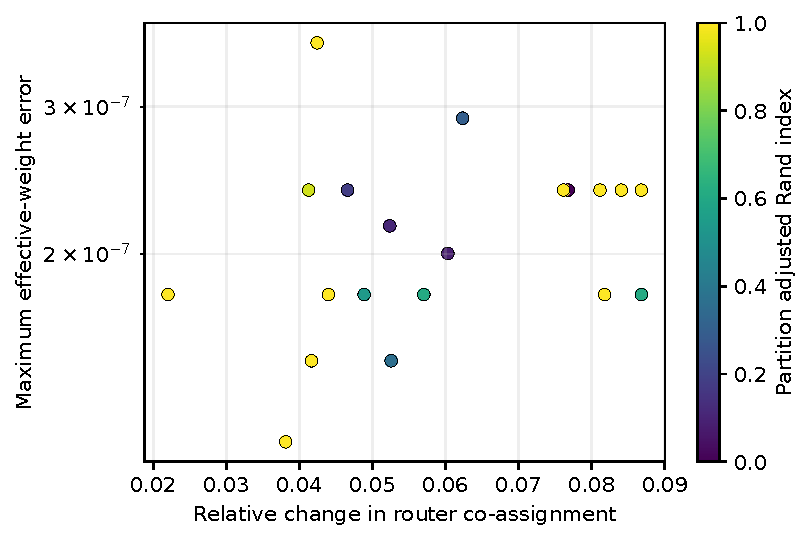
\includegraphics[width=\linewidth]{figures/gauge_equivalence.pdf}
    \caption{Gauge-equivalent routers.}
  \end{subfigure}\hfill
  \begin{subfigure}[t]{.48\linewidth}
    \centering
    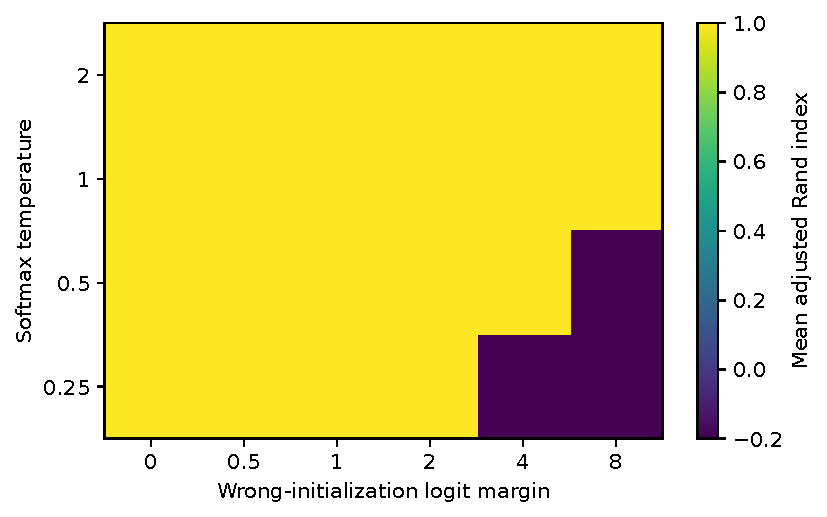
\includegraphics[width=\linewidth]{figures/saturation_recovery.pdf}
    \caption{Recovery from a wrong router.}
  \end{subfigure}
  \caption{Synthetic theory checks.  Effective weights remain equal at
  numerical precision while router summaries can change; saturation can
  suppress recovery from a deliberately wrong initialization.}
  \label{fig:gauge-saturation}
\end{figure}
}{}

The exact-factorization and distillation sweeps show that, for the tested
planted teachers and budgets, similar reconstruction or task loss need not
select the same router graph.  They are possibility and path-dependence checks,
not estimates of real-world frequency.  Discrete clustering succeeds when its
one-hot model matches the teacher, which is a positive control rather than a
general recovery guarantee.

\IfFileExists{generated/gauge_table.tex}{% Auto-generated by experiments/analyze_results.py; do not edit by hand.
\begin{table}[H]
\centering
\small
\caption{Gauge counterfactuals. Values are mean $\pm$ sample standard deviation across trials.}
\label{tab:gauge}
\begin{tabular}{lrr}
\toprule
Metric & Value & $n$ \\
\midrule
Effective max error & $2.11\!\times\!10^{-7} \pm 5.41\!\times\!10^{-8}$ & 20 \\
Argmax-partition ARI & $0.686 \pm 0.380$ & 20 \\
Co-assignment relative change & $0.059 \pm 0.019$ & 20 \\
Post-step effective relative difference & $0.002 \pm 9.90\!\times\!10^{-4}$ & 20 \\
\bottomrule
\end{tabular}
\end{table}
}{}
\IfFileExists{generated/saturation_table.tex}{% Auto-generated by experiments/analyze_results.py; do not edit by hand.
\begin{table}[H]
\centering
\scriptsize
\caption{Softmax-saturation sweep. Values are aggregated across seeds for each temperature and wrong-initialization margin.}
\label{tab:saturation}
\begin{tabular}{rrrrrr}
\toprule
Temperature & Margin & Initial grad. & Final MSE & ARI & $n$ \\
\midrule
0.250 & 0 & $0.008 \pm 4.18\!\times\!10^{-5}$ & $8.07\!\times\!10^{-8} \pm 2.96\!\times\!10^{-10}$ & $1.000 \pm 0$ & 5 \\
0.250 & 0.500 & $0.002 \pm 1.04\!\times\!10^{-10}$ & $7.88\!\times\!10^{-8} \pm 2.08\!\times\!10^{-13}$ & $1.000 \pm 0$ & 5 \\
0.250 & 1.000 & $4.62\!\times\!10^{-5} \pm 1.63\!\times\!10^{-12}$ & $6.00\!\times\!10^{-8} \pm 1.86\!\times\!10^{-13}$ & $1.000 \pm 0$ & 5 \\
0.250 & 2.000 & $1.55\!\times\!10^{-8} \pm 7.94\!\times\!10^{-16}$ & $1.94\!\times\!10^{-8} \pm 9.27\!\times\!10^{-14}$ & $1.000 \pm 0$ & 5 \\
0.250 & 4.000 & $9.14\!\times\!10^{-16} \pm 1.16\!\times\!10^{-22}$ & $0.021 \pm 2.28\!\times\!10^{-9}$ & $-0.222 \pm 3.10\!\times\!10^{-17}$ & 5 \\
0.250 & 8.000 & $0 \pm 0$ & $0.021 \pm 2.28\!\times\!10^{-9}$ & $-0.222 \pm 3.10\!\times\!10^{-17}$ & 5 \\
0.500 & 0 & $0.004 \pm 8.64\!\times\!10^{-6}$ & $2.52\!\times\!10^{-7} \pm 6.31\!\times\!10^{-10}$ & $1.000 \pm 0$ & 5 \\
0.500 & 0.500 & $0.004 \pm 2.65\!\times\!10^{-10}$ & $2.68\!\times\!10^{-7} \pm 4.13\!\times\!10^{-13}$ & $1.000 \pm 0$ & 5 \\
0.500 & 1.000 & $0.001 \pm 5.21\!\times\!10^{-11}$ & $2.76\!\times\!10^{-7} \pm 2.96\!\times\!10^{-13}$ & $1.000 \pm 0$ & 5 \\
0.500 & 2.000 & $2.31\!\times\!10^{-5} \pm 8.13\!\times\!10^{-13}$ & $2.49\!\times\!10^{-7} \pm 3.02\!\times\!10^{-13}$ & $1.000 \pm 0$ & 5 \\
0.500 & 4.000 & $7.74\!\times\!10^{-9} \pm 3.97\!\times\!10^{-16}$ & $1.44\!\times\!10^{-7} \pm 9.62\!\times\!10^{-14}$ & $1.000 \pm 0$ & 5 \\
0.500 & 8.000 & $4.57\!\times\!10^{-16} \pm 5.80\!\times\!10^{-23}$ & $0.021 \pm 2.28\!\times\!10^{-9}$ & $-0.222 \pm 3.10\!\times\!10^{-17}$ & 5 \\
1.000 & 0 & $0.002 \pm 1.73\!\times\!10^{-6}$ & $7.25\!\times\!10^{-7} \pm 7.43\!\times\!10^{-10}$ & $1.000 \pm 0$ & 5 \\
1.000 & 0.500 & $0.002 \pm 2.85\!\times\!10^{-10}$ & $7.17\!\times\!10^{-7} \pm 4.67\!\times\!10^{-13}$ & $1.000 \pm 0$ & 5 \\
1.000 & 1.000 & $0.002 \pm 1.33\!\times\!10^{-10}$ & $7.58\!\times\!10^{-7} \pm 5.92\!\times\!10^{-13}$ & $1.000 \pm 0$ & 5 \\
1.000 & 2.000 & $5.41\!\times\!10^{-4} \pm 2.60\!\times\!10^{-11}$ & $7.66\!\times\!10^{-7} \pm 3.52\!\times\!10^{-13}$ & $1.000 \pm 0$ & 5 \\
1.000 & 4.000 & $1.16\!\times\!10^{-5} \pm 4.07\!\times\!10^{-13}$ & $6.68\!\times\!10^{-7} \pm 6.33\!\times\!10^{-13}$ & $1.000 \pm 0$ & 5 \\
1.000 & 8.000 & $3.87\!\times\!10^{-9} \pm 1.99\!\times\!10^{-16}$ & $4.91\!\times\!10^{-7} \pm 1.19\!\times\!10^{-12}$ & $1.000 \pm 0$ & 5 \\
2.000 & 0 & $9.76\!\times\!10^{-4} \pm 1.81\!\times\!10^{-7}$ & $2.13\!\times\!10^{-6} \pm 4.74\!\times\!10^{-10}$ & $1.000 \pm 0$ & 5 \\
2.000 & 0.500 & $9.90\!\times\!10^{-4} \pm 8.23\!\times\!10^{-11}$ & $2.10\!\times\!10^{-6} \pm 1.15\!\times\!10^{-12}$ & $1.000 \pm 0$ & 5 \\
2.000 & 1.000 & $0.001 \pm 1.43\!\times\!10^{-10}$ & $2.09\!\times\!10^{-6} \pm 1.19\!\times\!10^{-12}$ & $1.000 \pm 0$ & 5 \\
2.000 & 2.000 & $9.09\!\times\!10^{-4} \pm 6.64\!\times\!10^{-11}$ & $2.19\!\times\!10^{-6} \pm 2.68\!\times\!10^{-12}$ & $1.000 \pm 0$ & 5 \\
2.000 & 4.000 & $2.71\!\times\!10^{-4} \pm 1.30\!\times\!10^{-11}$ & $2.17\!\times\!10^{-6} \pm 3.48\!\times\!10^{-12}$ & $1.000 \pm 0$ & 5 \\
2.000 & 8.000 & $5.78\!\times\!10^{-6} \pm 2.03\!\times\!10^{-13}$ & $1.82\!\times\!10^{-6} \pm 9.90\!\times\!10^{-13}$ & $1.000 \pm 0$ & 5 \\
\bottomrule
\end{tabular}
\end{table}
}{}
\IfFileExists{generated/factorization_full_table.tex}{%
  % Auto-generated by experiments/analyze_results.py; do not edit by hand.
\begin{table}[H]
\centering
\scriptsize
\caption{Exact-factorization results for cycle teachers. Values are mean $\pm$ sample standard deviation across seeds.}
\label{tab:factorization-full}
\resizebox{\linewidth}{!}{%
\begin{tabular}{lllrrrr}
\toprule
Method & Init relation & Raw init & Rel.\ error & ARI & Assignment acc. & $n$ \\
\midrule
k-means & neutral & neutral & $0 \pm 0$ & $1.000 \pm 0$ & $1.000 \pm 0$ & 10 \\
oracle & neutral & neutral & $0 \pm 0$ & $1.000 \pm 0$ & $1.000 \pm 0$ & 10 \\
soft & matched & cycle & $0.003 \pm 8.36\!\times\!10^{-4}$ & $1.000 \pm 0$ & $1.000 \pm 0$ & 10 \\
soft & mismatched & contiguous & $0.004 \pm 7.92\!\times\!10^{-4}$ & $0.636 \pm 0.158$ & $0.725 \pm 0.142$ & 10 \\
soft & neutral & neutral & $0.004 \pm 9.08\!\times\!10^{-4}$ & $0.894 \pm 0.171$ & $0.925 \pm 0.121$ & 10 \\
soft & random & random & $0.005 \pm 0.002$ & $0.894 \pm 0.171$ & $0.925 \pm 0.121$ & 10 \\
straight-through & matched & cycle & $0.004 \pm 0.001$ & $1.000 \pm 0$ & $1.000 \pm 0$ & 10 \\
straight-through & mismatched & contiguous & $0.009 \pm 0.025$ & $1.000 \pm 0$ & $1.000 \pm 0$ & 10 \\
straight-through & neutral & neutral & $8.44\!\times\!10^{-4} \pm 9.05\!\times\!10^{-4}$ & $1.000 \pm 0$ & $1.000 \pm 0$ & 10 \\
straight-through & random & random & $0.006 \pm 0.015$ & $1.000 \pm 0$ & $1.000 \pm 0$ & 10 \\
vertex-hard & matched & cycle & $0.005 \pm 0.002$ & $1.000 \pm 0$ & $1.000 \pm 0$ & 10 \\
vertex-hard & mismatched & contiguous & $0.854 \pm 0.001$ & $-0.222 \pm 2.93\!\times\!10^{-17}$ & $0.333 \pm 0$ & 10 \\
vertex-hard & neutral & neutral & $4.93\!\times\!10^{-4} \pm 3.89\!\times\!10^{-5}$ & $1.000 \pm 0$ & $1.000 \pm 0$ & 10 \\
vertex-hard & random & random & $0.475 \pm 0.271$ & $0.523 \pm 0.333$ & $0.783 \pm 0.172$ & 10 \\
\bottomrule
\end{tabular}%
}
\end{table}
\begin{table}[H]
\centering
\scriptsize
\caption{Exact-factorization results for contiguous teachers. Values are mean $\pm$ sample standard deviation across seeds.}
\label{tab:factorization-full-contiguous}
\resizebox{\linewidth}{!}{%
\begin{tabular}{lllrrrr}
\toprule
Method & Init relation & Raw init & Rel.\ error & ARI & Assignment acc. & $n$ \\
\midrule
k-means & neutral & neutral & $0 \pm 0$ & $1.000 \pm 0$ & $1.000 \pm 0$ & 10 \\
oracle & neutral & neutral & $0 \pm 0$ & $1.000 \pm 0$ & $1.000 \pm 0$ & 10 \\
soft & matched & contiguous & $0.003 \pm 8.04\!\times\!10^{-4}$ & $1.000 \pm 0$ & $1.000 \pm 0$ & 10 \\
soft & mismatched & cycle & $0.004 \pm 6.87\!\times\!10^{-4}$ & $0.636 \pm 0.158$ & $0.725 \pm 0.142$ & 10 \\
soft & neutral & neutral & $0.005 \pm 0.001$ & $0.929 \pm 0.150$ & $0.950 \pm 0.105$ & 10 \\
soft & random & random & $0.006 \pm 0.003$ & $0.929 \pm 0.150$ & $0.950 \pm 0.105$ & 10 \\
straight-through & matched & contiguous & $0.004 \pm 0.001$ & $1.000 \pm 0$ & $1.000 \pm 0$ & 10 \\
straight-through & mismatched & cycle & $0.009 \pm 0.025$ & $1.000 \pm 0$ & $1.000 \pm 0$ & 10 \\
straight-through & neutral & neutral & $0.006 \pm 0.016$ & $1.000 \pm 0$ & $1.000 \pm 0$ & 10 \\
straight-through & random & random & $0.004 \pm 0.005$ & $1.000 \pm 0$ & $1.000 \pm 0$ & 10 \\
vertex-hard & matched & contiguous & $0.005 \pm 0.002$ & $1.000 \pm 0$ & $1.000 \pm 0$ & 10 \\
vertex-hard & mismatched & cycle & $0.855 \pm 0.002$ & $-0.222 \pm 2.93\!\times\!10^{-17}$ & $0.333 \pm 0$ & 10 \\
vertex-hard & neutral & neutral & $5.21\!\times\!10^{-4} \pm 6.09\!\times\!10^{-5}$ & $1.000 \pm 0$ & $1.000 \pm 0$ & 10 \\
vertex-hard & random & random & $0.492 \pm 0.220$ & $0.525 \pm 0.297$ & $0.792 \pm 0.153$ & 10 \\
\bottomrule
\end{tabular}%
}
\end{table}
\begin{table}[H]
\centering
\scriptsize
\caption{Exact-factorization results for palindrome teachers. Values are mean $\pm$ sample standard deviation across seeds.}
\label{tab:factorization-full-palindrome}
\resizebox{\linewidth}{!}{%
\begin{tabular}{lllrrrr}
\toprule
Method & Init relation & Raw init & Rel.\ error & ARI & Assignment acc. & $n$ \\
\midrule
k-means & neutral & neutral & $0 \pm 0$ & $1.000 \pm 0$ & $1.000 \pm 0$ & 10 \\
oracle & neutral & neutral & $0 \pm 0$ & $1.000 \pm 0$ & $1.000 \pm 0$ & 10 \\
soft & neutral & neutral & $0.007 \pm 0.006$ & $0.940 \pm 0.126$ & $0.967 \pm 0.070$ & 10 \\
soft & random & random & $0.005 \pm 0.002$ & $0.910 \pm 0.145$ & $0.950 \pm 0.081$ & 10 \\
soft & structured-other & contiguous & $0.004 \pm 6.92\!\times\!10^{-4}$ & $0.970 \pm 0.095$ & $0.983 \pm 0.053$ & 10 \\
soft & structured-other & cycle & $0.004 \pm 7.73\!\times\!10^{-4}$ & $0.940 \pm 0.126$ & $0.967 \pm 0.070$ & 10 \\
straight-through & neutral & neutral & $9.97\!\times\!10^{-4} \pm 5.35\!\times\!10^{-4}$ & $1.000 \pm 0$ & $1.000 \pm 0$ & 10 \\
straight-through & random & random & $0.046 \pm 0.128$ & $0.969 \pm 0.098$ & $0.975 \pm 0.079$ & 10 \\
straight-through & structured-other & contiguous & $0.010 \pm 0.026$ & $1.000 \pm 0$ & $1.000 \pm 0$ & 10 \\
straight-through & structured-other & cycle & $0.002 \pm 9.25\!\times\!10^{-4}$ & $1.000 \pm 0$ & $1.000 \pm 0$ & 10 \\
vertex-hard & neutral & neutral & $0.092 \pm 0.201$ & $0.936 \pm 0.163$ & $0.958 \pm 0.106$ & 10 \\
vertex-hard & random & random & $0.604 \pm 0.136$ & $0.359 \pm 0.237$ & $0.708 \pm 0.132$ & 10 \\
vertex-hard & structured-other & contiguous & $0.907 \pm 0.001$ & $-0.243 \pm 0$ & $0.333 \pm 0$ & 10 \\
vertex-hard & structured-other & cycle & $0.795 \pm 4.82\!\times\!10^{-4}$ & $0.139 \pm 2.93\!\times\!10^{-17}$ & $0.500 \pm 0$ & 10 \\
\bottomrule
\end{tabular}%
}
\end{table}
\begin{table}[H]
\centering
\scriptsize
\caption{Exact-factorization results for random balanced teachers. Values are mean $\pm$ sample standard deviation across seeds.}
\label{tab:factorization-full-random-balanced}
\resizebox{\linewidth}{!}{%
\begin{tabular}{lllrrrr}
\toprule
Method & Init relation & Raw init & Rel.\ error & ARI & Assignment acc. & $n$ \\
\midrule
k-means & neutral & neutral & $0 \pm 0$ & $1.000 \pm 0$ & $1.000 \pm 0$ & 10 \\
oracle & neutral & neutral & $0 \pm 0$ & $1.000 \pm 0$ & $1.000 \pm 0$ & 10 \\
soft & neutral & neutral & $0.005 \pm 0.002$ & $0.858 \pm 0.183$ & $0.900 \pm 0.129$ & 10 \\
soft & random & random & $0.007 \pm 0.003$ & $0.856 \pm 0.254$ & $0.900 \pm 0.175$ & 10 \\
soft & structured-other & contiguous & $0.004 \pm 9.89\!\times\!10^{-4}$ & $0.818 \pm 0.311$ & $0.875 \pm 0.212$ & 10 \\
soft & structured-other & cycle & $0.003 \pm 6.11\!\times\!10^{-4}$ & $0.965 \pm 0.112$ & $0.975 \pm 0.079$ & 10 \\
straight-through & neutral & neutral & $5.97\!\times\!10^{-4} \pm 2.50\!\times\!10^{-4}$ & $1.000 \pm 0$ & $1.000 \pm 0$ & 10 \\
straight-through & random & random & $0.105 \pm 0.209$ & $0.919 \pm 0.173$ & $0.942 \pm 0.125$ & 10 \\
straight-through & structured-other & contiguous & $0.004 \pm 0.007$ & $1.000 \pm 0$ & $1.000 \pm 0$ & 10 \\
straight-through & structured-other & cycle & $0.002 \pm 0.001$ & $1.000 \pm 0$ & $1.000 \pm 0$ & 10 \\
vertex-hard & neutral & neutral & $5.00\!\times\!10^{-4} \pm 4.46\!\times\!10^{-5}$ & $1.000 \pm 0$ & $1.000 \pm 0$ & 10 \\
vertex-hard & random & random & $0.493 \pm 0.279$ & $0.497 \pm 0.343$ & $0.775 \pm 0.162$ & 10 \\
vertex-hard & structured-other & contiguous & $0.796 \pm 0.061$ & $-0.039 \pm 0.172$ & $0.475 \pm 0.125$ & 10 \\
vertex-hard & structured-other & cycle & $0.785 \pm 0.050$ & $-0.019 \pm 0.127$ & $0.492 \pm 0.100$ & 10 \\
\bottomrule
\end{tabular}%
}
\end{table}
\begin{table}[H]
\centering
\scriptsize
\caption{Exact-factorization results for imbalanced teachers. Values are mean $\pm$ sample standard deviation across seeds.}
\label{tab:factorization-full-imbalanced}
\resizebox{\linewidth}{!}{%
\begin{tabular}{lllrrrr}
\toprule
Method & Init relation & Raw init & Rel.\ error & ARI & Assignment acc. & $n$ \\
\midrule
k-means & neutral & neutral & $0 \pm 0$ & $1.000 \pm 0$ & $1.000 \pm 0$ & 10 \\
oracle & neutral & neutral & $0 \pm 0$ & $1.000 \pm 0$ & $1.000 \pm 0$ & 10 \\
soft & neutral & neutral & $0.006 \pm 0.004$ & $0.997 \pm 0.010$ & $0.992 \pm 0.026$ & 10 \\
soft & random & random & $0.004 \pm 0.002$ & $0.960 \pm 0.086$ & $0.958 \pm 0.044$ & 10 \\
soft & structured-other & contiguous & $0.004 \pm 9.57\!\times\!10^{-4}$ & $1.000 \pm 0$ & $1.000 \pm 0$ & 10 \\
soft & structured-other & cycle & $0.289 \pm 2.68\!\times\!10^{-5}$ & $0.413 \pm 0.028$ & $0.617 \pm 0.043$ & 10 \\
straight-through & neutral & neutral & $0.008 \pm 0.013$ & $1.000 \pm 0$ & $1.000 \pm 0$ & 10 \\
straight-through & random & random & $0.216 \pm 0.150$ & $0.698 \pm 0.275$ & $0.800 \pm 0.181$ & 10 \\
straight-through & structured-other & contiguous & $0.030 \pm 0.050$ & $1.000 \pm 0$ & $1.000 \pm 0$ & 10 \\
straight-through & structured-other & cycle & $0.289 \pm 1.44\!\times\!10^{-4}$ & $0.440 \pm 0.017$ & $0.658 \pm 0.026$ & 10 \\
vertex-hard & neutral & neutral & $0.662 \pm 0.070$ & $0.090 \pm 0.101$ & $0.458 \pm 0.044$ & 10 \\
vertex-hard & random & random & $0.658 \pm 0.064$ & $0.078 \pm 0.098$ & $0.500 \pm 0.039$ & 10 \\
vertex-hard & structured-other & contiguous & $0.722 \pm 0.003$ & $-0.031 \pm 7.31\!\times\!10^{-18}$ & $0.500 \pm 0$ & 10 \\
vertex-hard & structured-other & cycle & $0.696 \pm 0.002$ & $0.026 \pm 0$ & $0.417 \pm 0$ & 10 \\
\bottomrule
\end{tabular}%
}
\end{table}

}{}
\IfFileExists{generated/distillation_full_table.tex}{%
  % Auto-generated by experiments/analyze_results.py; do not edit by hand.
\begin{table}[H]
\centering
\scriptsize
\caption{Full functional-distillation results by architecture, teacher pattern, and raw initialization. Values are mean $\pm$ sample standard deviation.}
\label{tab:distillation-full}
\resizebox{\linewidth}{!}{%
\begin{tabular}{llrrr}
\toprule
Student / init relation & Raw init & Test loss & ARI & $n$ \\
\midrule
MLP: contiguous / matched & pattern\_contiguous & $0.006 \pm 8.56\!\times\!10^{-5}$ & $1.000 \pm 0$ & 5 \\
MLP: contiguous / mismatched & pattern\_cycle & $0.006 \pm 7.00\!\times\!10^{-5}$ & $-0.167 \pm 0$ & 5 \\
MLP: contiguous / neutral & neutral & $0.012 \pm 1.99\!\times\!10^{-4}$ & $0.283 \pm 0.082$ & 5 \\
MLP: cycle / matched & pattern\_cycle & $0.005 \pm 6.21\!\times\!10^{-5}$ & $1.000 \pm 0$ & 5 \\
MLP: cycle / mismatched & pattern\_contiguous & $0.006 \pm 7.65\!\times\!10^{-5}$ & $-0.167 \pm 0$ & 5 \\
MLP: cycle / neutral & neutral & $0.012 \pm 1.85\!\times\!10^{-4}$ & $-0.226 \pm 0.056$ & 5 \\
MLP: palindrome / neutral & neutral & $0.011 \pm 2.24\!\times\!10^{-4}$ & $-0.077 \pm 0.062$ & 5 \\
MLP: palindrome / structured\_other & pattern\_contiguous & $0.005 \pm 1.27\!\times\!10^{-4}$ & $-0.189 \pm 0$ & 5 \\
MLP: palindrome / structured\_other & pattern\_cycle & $0.005 \pm 9.60\!\times\!10^{-5}$ & $0.075 \pm 0$ & 5 \\
MLP: random\_balanced / neutral & neutral & $0.012 \pm 1.91\!\times\!10^{-4}$ & $-0.053 \pm 0.130$ & 5 \\
MLP: random\_balanced / structured\_other & pattern\_contiguous & $0.006 \pm 9.98\!\times\!10^{-5}$ & $-0.108 \pm 0.130$ & 5 \\
MLP: random\_balanced / structured\_other & pattern\_cycle & $0.006 \pm 6.30\!\times\!10^{-5}$ & $-0.050 \pm 0.261$ & 5 \\
Transformer: contiguous / matched & pattern\_contiguous & $4.03\!\times\!10^{-4} \pm 9.10\!\times\!10^{-5}$ & $1.000 \pm 0$ & 5 \\
Transformer: contiguous / mismatched & pattern\_cycle & $4.09\!\times\!10^{-4} \pm 9.89\!\times\!10^{-5}$ & $-0.167 \pm 0$ & 5 \\
Transformer: contiguous / neutral & neutral & $5.24\!\times\!10^{-4} \pm 1.30\!\times\!10^{-4}$ & $0.205 \pm 0.050$ & 5 \\
Transformer: cycle / matched & pattern\_cycle & $3.90\!\times\!10^{-4} \pm 6.52\!\times\!10^{-5}$ & $1.000 \pm 0$ & 5 \\
Transformer: cycle / mismatched & pattern\_contiguous & $4.04\!\times\!10^{-4} \pm 7.90\!\times\!10^{-5}$ & $-0.167 \pm 0$ & 5 \\
Transformer: cycle / neutral & neutral & $4.98\!\times\!10^{-4} \pm 9.52\!\times\!10^{-5}$ & $-0.032 \pm 0.122$ & 5 \\
Transformer: palindrome / neutral & neutral & $4.99\!\times\!10^{-4} \pm 8.18\!\times\!10^{-5}$ & $-0.091 \pm 0.032$ & 5 \\
Transformer: palindrome / structured\_other & pattern\_contiguous & $4.20\!\times\!10^{-4} \pm 6.29\!\times\!10^{-5}$ & $-0.189 \pm 0$ & 5 \\
Transformer: palindrome / structured\_other & pattern\_cycle & $3.93\!\times\!10^{-4} \pm 5.14\!\times\!10^{-5}$ & $0.075 \pm 0$ & 5 \\
Transformer: random\_balanced / neutral & neutral & $4.72\!\times\!10^{-4} \pm 1.11\!\times\!10^{-4}$ & $0.007 \pm 0.159$ & 5 \\
Transformer: random\_balanced / structured\_other & pattern\_contiguous & $3.91\!\times\!10^{-4} \pm 7.13\!\times\!10^{-5}$ & $-0.108 \pm 0.130$ & 5 \\
Transformer: random\_balanced / structured\_other & pattern\_cycle & $3.76\!\times\!10^{-4} \pm 7.10\!\times\!10^{-5}$ & $-0.050 \pm 0.261$ & 5 \\
\bottomrule
\end{tabular}%
}
\end{table}

}{}

\IfFileExists{figures/factorization_loss_vs_ari.pdf}{%
\begin{figure}[H]
  \centering
  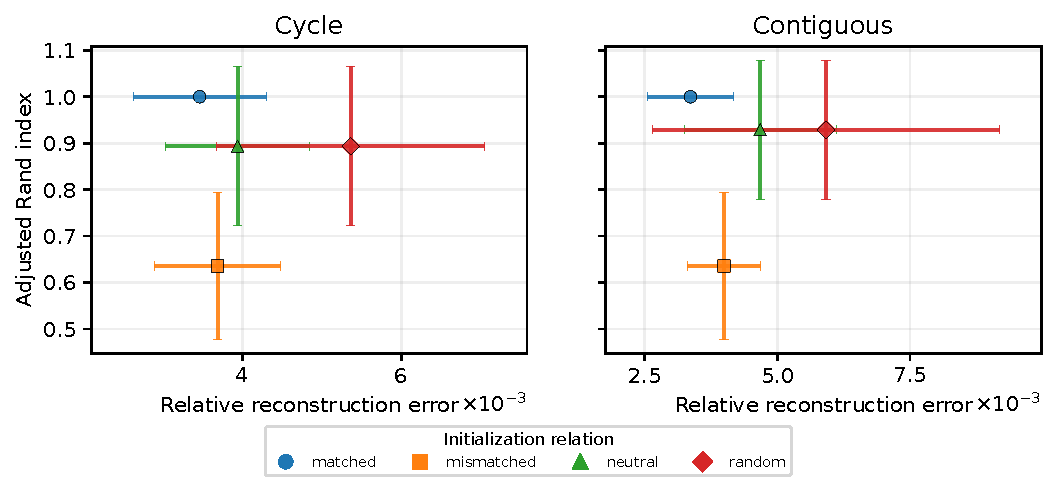
\includegraphics[width=.72\linewidth]{figures/factorization_loss_vs_ari.pdf}
  \caption{Soft-router exact-factorization runs for cycle and contiguous
  teachers.  Reconstruction error and planted-graph recovery are separate
  axes.}
  \label{fig:factorization}
\end{figure}
}{}

\IfFileExists{figures/distillation_loss_vs_ari.pdf}{%
\begin{figure}[H]
  \centering
  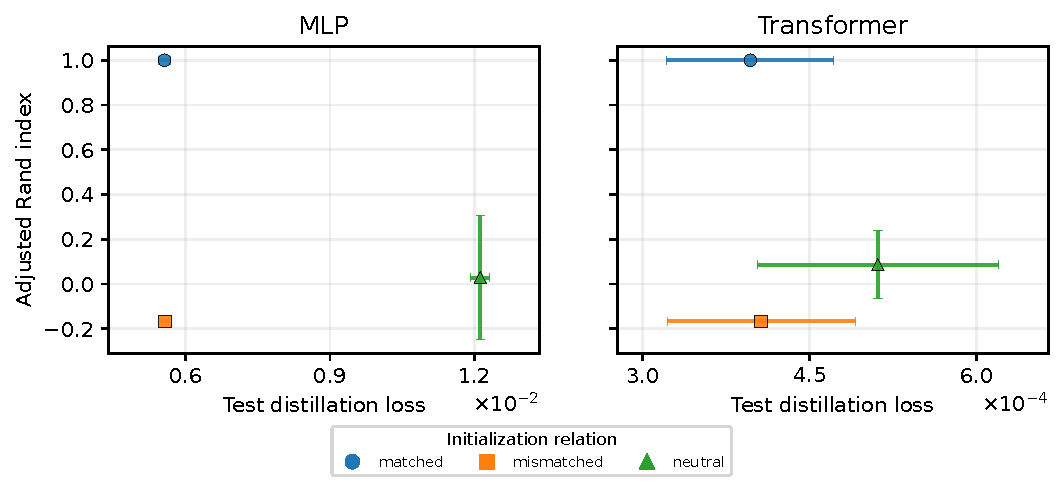
\includegraphics[width=.72\linewidth]{figures/distillation_loss_vs_ari.pdf}
  \caption{Distillation loss versus planted-graph ARI for the residual MLP and
  causal Transformer sanity checks.}
  \label{fig:distillation}
\end{figure}
}{}

\IfFileExists{generated/probe_table.tex}{% Auto-generated by experiments/analyze_results.py; do not edit by hand.
\begin{table}[H]
\centering
\small
\caption{Paired probe recovery aggregated over probe counts, fixed additive-noise levels, graphs, and seeds. Functional modes share inputs, noise, and projection. The visible-effective-parameter baseline uses neither observation noise nor projection and is not a test of functional equivalence. Values are mean $\pm$ sample standard deviation.}
\label{tab:probes}
\begin{tabular}{llrrr}
\toprule
Architecture & Signature & ARI & Empirical gap & $n$ \\
\midrule
MLP & shared input & $0.676 \pm 0.432$ & $-27.192 \pm 66.232$ & 1680 \\
MLP & native & $0.675 \pm 0.434$ & $-27.293 \pm 66.173$ & 1680 \\
MLP & effective parameter & $1.000 \pm 0$ & $0.008 \pm 5.82\!\times\!10^{-5}$ & 1680 \\
Transformer & shared input & $0.501 \pm 0.471$ & $-88.706 \pm 190.527$ & 1680 \\
Transformer & native & $0.501 \pm 0.470$ & $-88.758 \pm 190.490$ & 1680 \\
Transformer & effective parameter & $1.000 \pm 0$ & $0.009 \pm 2.08\!\times\!10^{-5}$ & 1680 \\
\bottomrule
\end{tabular}
\end{table}
}{}
\IfFileExists{figures/probe_phase_diagram.pdf}{%
\begin{figure}[H]
  \centering
  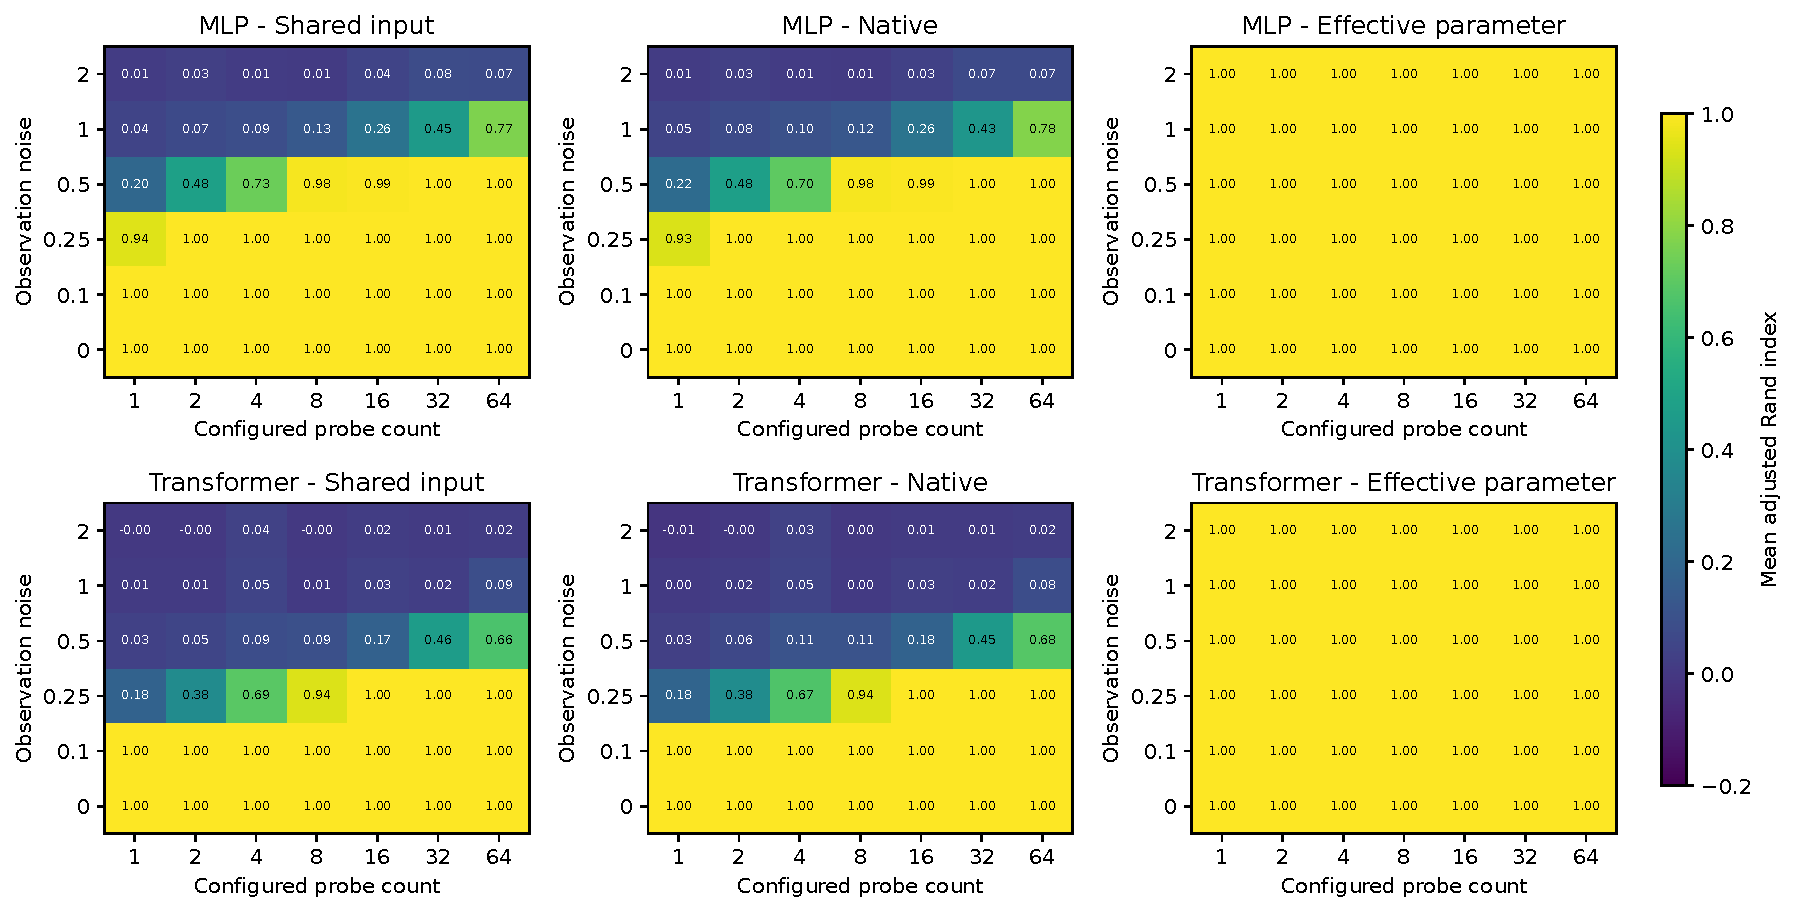
\includegraphics[width=.96\linewidth]{figures/probe_phase_diagram.pdf}
  \caption{Shared-input, native-signature, and visible-effective-parameter
  recovery as probe count and fixed additive observation noise vary.  The
  parameter baseline is repeated across the grid only for comparison and is
  not a functional-equivalence test.  This is a planted-partition sanity check,
  not evidence of superiority on natural systems.}
  \label{fig:probes}
\end{figure}
}{}

Functional-signature recovery generally improves with probe count and degrades
with observation noise.  The empirical within/between gap is computed against
the planted partition, rather than against the predicted clusters, but remains
only a finite-sample diagnostic unless the theorem's population gap and uniform
concentration assumptions are justified for this observation model.

\section{Language-model stability results}
\label{app:language-results}

\IfFileExists{generated/language_table.tex}{%
  % Auto-generated by experiments/analyze_results.py; do not edit by hand.
\begin{table}[H]
\centering
\small
\caption{Language-model stress test. BPB is estimated from 100 seeded, sampled test batches. Values are mean $\pm$ sample standard deviation across seeds; pairwise ARI descriptively summarizes the three dependent run pairs.}
\label{tab:language}
\begin{tabular}{lrrrr}
\toprule
Initialization & Sampled test BPB & L1 movement & Pairwise ARI & $n$ \\
\midrule
neutral & $2.415 \pm 0.009$ & $0.012 \pm 0.003$ & $0.099 \pm 0.157$ & 3 \\
pattern\_contiguous & $2.111 \pm 0.008$ & $3.10\!\times\!10^{-4} \pm 1.35\!\times\!10^{-5}$ & $1.000 \pm 0$ & 3 \\
pattern\_cycle & $2.181 \pm 0.011$ & $3.50\!\times\!10^{-4} \pm 4.60\!\times\!10^{-5}$ & $1.000 \pm 0$ & 3 \\
random & $2.319 \pm 0.015$ & $0.065 \pm 0.008$ & $-0.045 \pm 0.112$ & 3 \\
\bottomrule
\end{tabular}
\end{table}

}{The aggregate language-model table is generated by the analysis script.}

Distinct structured initializations can retain their partitions while reaching
competitive BPB.  With no privileged natural-language graph, this is evidence
of initialization dependence, not evidence that either retained partition is
false or historically correct.  The one-of-three partition-fold witness in
Table~\ref{tab:router-decision} is reported separately and does not convert this
stability arm into a prevalence result.

\section{Reproducibility checklist}

The response summary validates source hashes, checkpoint hashes, rank
assumptions, analytic/native formula agreement, the permutation control, and
all fixed probe outcomes.  The separate tomography summary validates three
newly generated raw artifacts, exact-gauge/common-design gates, rank and
dimension conditions, component reconstruction, and the permutation and
non-permutation controls without changing the older response generator.  The ASLoRA summary validates a common protocol hash,
generation-time source hashes, complete declared candidate coverage, the
canonical equivalence gate, and exact restoration for every seed and gauge.
The router-decision summary retains both exhausted searches, their full funnel
counts, checkpoint hashes, and the paired successful-seed evaluation; unlike
the other three summaries, it does not itself contain a generation-source-hash
attestation, so we do not claim equal provenance strength.

The artifact additionally includes deterministic seed handling, raw JSON
records, executable summarizers, the script that generates the three original audit
LaTeX tables and their appendix details from validated summaries, tests for summary-gate failures,
and unit tests for causal masking, permutation-invariant metrics, gauge
equivalence, response formulas, structured response reconstruction and its
approximate-product rejection boundary, restoration, and probe recovery.  Dataset
download is separated from training and accesses no private data.

\section{Prospective enhancement protocols and numerical limits}
\label{app:enhancement-experiments}

\subsection{Historical byte-LM witness}
\label{app:historical-fold-witness}

% Auto-generated by experiments/generate_paper_audit_tables.py; do not edit.
% Source: results/router_decisions_summary.json
% Source SHA256: 0e863e1db624a7f25697a7a6873e83e91f928458ba61cdfd06081e582b3e28f2
\providecommand{\RouterSearchSuccesses}{1}
\providecommand{\RouterSearchSeeds}{3}
\providecommand{\RouterSearchTrials}{5000}
\providecommand{\RouterGroupBudget}{4}
\providecommand{\RouterWitnessDeltaBPB}{2.6396}
\providecommand{\RouterWitnessCILower}{2.6287}
\providecommand{\RouterWitnessCIUpper}{2.6510}
\providecommand{\RouterWitnessCandidateBPB}{4.8149}
\providecommand{\RouterWitnessUnigramBPB}{4.6242}
\providecommand{\RouterWitnessKMeansBPB}{2.1753}
\providecommand{\RouterWitnessWardBPB}{2.1753}
\providecommand{\RouterUnevaluatedSeeds}{2}
\begin{table}[H]
\centering
\small
\setlength{\tabcolsep}{3pt}
\caption{Finite same-group-budget partition-fold search at trained, initialization-dominated byte-LM checkpoints.  ``Not found'' means the predeclared finite search exhausted; it is not a non-existence claim.  Fold BPB compares partitions refit from the same effective tensors.  The sole measurable consequence was not replicated under the same search (one witness in three seeds).}
\label{tab:router-decision}
\begin{tabular}{@{}clccc@{}}
\toprule
Seed & Search & Fold BPB ref.$\to$cand. & $\Delta$BPB [95\% CI] & Replicated? \\
\midrule
0 & found & 2.175$\to$4.815 & $+2.640\;[+2.629,+2.651]$ & no (1/3) \\
1 & not found & -- & -- & no (1/3) \\
2 & not found & -- & -- & no (1/3) \\
\bottomrule
\end{tabular}
\end{table}


The original fixed-budget search succeeds at one of three checkpoints;
all three routers are initialization-dominated. The successful candidate
changes group sizes from $3/3/3/3$ to $5/3/3/1$, so its large BPB difference
does not isolate membership from balance. Failed searches store no downstream
fold or baseline evaluation. The detailed historical protocol and conditional
interval interpretation remain in Appendix~\ref{app:experimental-details}.
The new equal-size experiments below are separately registered evidence.

\paragraph{Training and matched decision budgets.}
The extension uses fresh seeds 10--12, width 128, MLP width 512, 12 layers,
four bases, eight heads, context 128 and batch size 16. AdamW uses base
learning rate $3\times10^{-4}$, router multiplier ten, 300 warmup steps,
cosine decay to one tenth, weight decay 0.1 for weights and zero for routers,
and BF16 autocast. There is no routing regularizer or temperature annealing.
Only the fixed final step 6,000 is audited; a separate 100-step seed-90
validation-only pilot checked implementation and timing. This configuration
differs from the original checkpoints and is not a controlled comparison of
training lengths. Router movement and validation curves do not alone prove
convergence or task-essential routing.

The positive-stochastic and signed-local families retain the previously
specified distributions and condition-number bound 30; the new legality gate
requires identical sorted group sizes. Selection sees router probabilities
only. Test evaluation uses 64 disjoint batches of eight 128-token sequences,
with identical stored starts for every action. Recovery uses 500 updates at
learning rate $10^{-4}$, fresh AdamW state, weight decay 0.1 and clipping norm
one, evaluated at steps 0,100,500. The hard routing assignments are frozen;
inactive stored slots are retained, so no latency or realized storage saving
is claimed. The fixed-size effective-parameter comparator uses 16 seeded
restarts and at most 50 improving pair swaps per restart to minimize centroid
SSE. It is a local search, not a global optimum or a task-loss optimizer.
Unconstrained Ward is included descriptively, since its group sizes may differ.

\paragraph{Natural-gradient measurement.}
Each checkpoint contributes 16 training minibatches of two 32-token sequences.
The effective-weight forward matches the native model, and its gradients,
pulled back through the factor map, match the native factor gradients.
For numerical conditioning, each direction and its measured response receive
the same normalization. The complement Gram and local linear systems in
Appendix~\ref{app:natural-tomography} use a fixed relative pseudoinverse cutoff
$10^{-12}$. Factor recovery retains the original fixed diagonalization weights.
All ranks, spectra, component errors, held-out predictions, unsuccessful
low-probe reconstructions and finite-step measurements are stored.
The last four directions are held out for every $q$; larger fits are nested,
so these measurements are not independent training replicates.

\paragraph{Joint noise and degeneracy.}
A prospective 450-cell FP64 synthetic grid uses ten seeds with $L=6,K=3,D=16$,
interior factors and contractions toward router rank loss or simplex vertices.
Relative product and response noise levels are
$0,10^{-8},10^{-6},10^{-4},10^{-2}$; common noise directions couple levels
within each cell. The observed product is truncated to rank $K$, its row
space supplies the designed probes, and the true response to those probes is
measured before adding response noise. This tests geometry estimation as well
as response error. All runs return factors, but this does not imply accurate
or feasible recovery: near rank loss, relative factor errors can exceed 60
already at $10^{-6}$ noise. Corollary~\ref{cor:joint-stability} requires valid,
uniformly nondegenerate factors and does not certify these unconstrained outputs.

\begin{figure}[t]
\centering
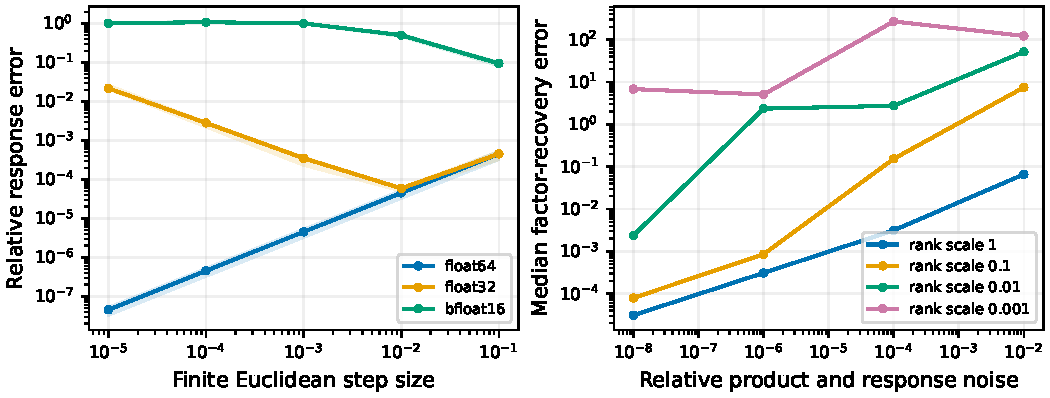
\includegraphics[width=\linewidth]{figures/enhancement_precision.pdf}
\caption{Two numerical limits. Left: finite-step response error at the three
new checkpoints; curves show medians and shading the observed seed range.
Smaller steps reduce FP64 truncation error but amplify low-precision
subtraction error. Right: median factor error over ten synthetic seeds as both
product and response observations are perturbed. The rank scale contracts
the router toward a rank-one uniform matrix; it is not a noise level.
These finite grids are diagnostic rather than worst-case guarantees.}
\label{fig:enhancement-precision}
\end{figure}

\paragraph{Artifacts and scope.}
Versioned protocols and source-bound raw records are supplied under
\texttt{research/} and \texttt{results/enhancement/}, including checkpoints,
seeds and corpus hashes. Each seed's paired bootstrap uses 10,000
resamples of its evaluation blocks; intervals are conditional and do not
substitute for independent training seeds. The new evidence supplements,
rather than overwrites, the original raw records and their negative findings.

\section{Frozen noisy-recovery and rejection study}
\label{app:trusted-experiments}

\paragraph{Prospective splits and observations.}
The local protocol and source freeze are
\texttt{research/TRUSTED\_RECOVERY\_PROTOCOL.md} and
\texttt{research/TRUSTED\_RECOVERY\_FREEZE.json}.
They are timestamped execution records, not an independent preregistration.
Development uses synthetic seeds 0--3 and existing byte-LM seed 10.
Calibration uses synthetic seeds 100--119 and newly trained byte-LM seeds
20--21; evaluation uses synthetic seeds 200--239 and new byte-LM seeds
22--25. The six fresh checkpoints use the unchanged width-128, $L=12$,
$K=4$, 6000-step configuration of the preceding controlled training study.
There is no checkpoint selection on recovery outcomes.

Synthetic factors have $L=6,K=3,D=16$, random-normal bases, and four router
regimes: interior softmax, contractions toward the uniform router by factors
$0.1$ and $0.01$, and a contraction toward balanced one-hot rows by $0.01$.
Each instance supplies 16 normalized Gaussian gradient directions.
Language directions are actual effective-parameter cross-entropy gradients
from 16 training-split minibatches of size $2\times32$, sampled with fixed
seed offset 3100000. Four or twelve initial directions fit the estimator;
the last four assess held-out response fit. Response observations come from
automatic differentiation of the factor map, without calling its closed-form
response formula.

Product and each response receive independently drawn Gaussian perturbation
directions rescaled to relative Frobenius norms
$\sigma\in\{0,10^{-8},10^{-6},10^{-4},10^{-3},10^{-2}\}$.
Directions are shared across noise levels within an instance.
The supplied bound $\sigma$ is known; the true perturbation vector and factors
are not supplied to recovery. The estimated rank-$K$ product row subspace
is used by all methods, and evaluation includes basis error outside it.
This observation-noise experiment does not model biased, adversarial,
quantized, or unknown optimizer-state errors.

\paragraph{Fixed estimators and observable scores.}
The projected spectral baseline clips router entries below $10^{-8}$,
normalizes rows, and refits the basis by least squares. Joint fitting uses
simplex logits in orthonormal zero-sum coordinates and normalized basis
coordinates, with SciPy trust-region reflective least squares and exact
forward-mode Jacobians. Three starts are fixed: projected spectral,
a $0.1$ logit perturbation, and a random simplex router. Each has a budget
of 80 function evaluations; the smallest observed training residual selects
the output. There is one developed solver variant, with no tuning on
calibration or evaluation factors.

All acceptance rules require a numerically feasible router and finite score.
The combined score is the maximum of (i) training plus held-out residual
plus twice the normalized noise budget, divided by the simplex-tangent
Jacobian's smallest singular value; (ii) an observed product-subspace
perturbation ratio; and (iii) permutation-aligned disagreement among
competitive starts for the joint fit. A separately disclosed $10^{-10}$
numerical floor enters the empirical noise budget.
The comparison scores use only residual or inverse Jacobian singular value.
Their implementation and thresholds are frozen, and no score uses truth
at prediction time.

For each method/score pair, one threshold is chosen on pooled calibration
data to maximize accepted count, subject to at least 20 accepted synthetic
outputs and at most $5\%$ bad among all accepted outputs. Ties are accepted
together. An infeasible threshold would reject all and be reported as a
failure. The same threshold transfers to both evaluation domains.
Good errors are at most $0.05$, bad errors exceed $0.10$, and intermediate
errors are reported separately. This empirical calibration is not a
distribution-free risk guarantee.

\begin{table}[t]
\centering
\small
\caption{Synthetic held-out diagnostic comparison (percent). Coverage is the accepted fraction; bad rejection is recall on errors $>0.10$; good rejection is false rejection on errors $\le0.05$; accepted bad is the bad fraction among accepted outputs. Each threshold was frozen using calibration only.}
\label{tab:trusted-diagnostics}
\begin{tabular}{llrrrr}
\toprule
Method & Score & Coverage & Bad reject & Good reject & Accepted bad \\
\midrule
Spectral & Combined & 10.21 & 100.00 & 85.04 & 0.00 \\
Spectral & Residual & 10.21 & 100.00 & 85.04 & 0.00 \\
Spectral & Condition & 10.26 & 100.00 & 84.96 & 0.00 \\
Projected & Combined & 72.71 & 90.11 & 0.00 & 4.01 \\
Projected & Residual & 72.66 & 92.23 & 0.00 & 3.15 \\
Projected & Condition & 21.30 & 98.06 & 70.48 & 2.69 \\
Joint fit & Combined & 92.81 & 59.47 & 0.18 & 5.16 \\
Joint fit & Residual & 91.51 & 70.04 & 0.18 & 3.87 \\
Joint fit & Condition & 24.32 & 91.63 & 72.73 & 4.07 \\
\bottomrule
\end{tabular}
\end{table}


\paragraph{Results, including unsuccessful diagnostics.}
All 1920 synthetic joint fits return; there are 1639 good, 54 intermediate,
and 227 bad outputs. Projected spectral recovery has three failed outputs,
all retained in the 1920-case denominator.
Seventy selected joint-fit runs exhaust their 80-evaluation budget; a returned
estimate is not a convergence claim. Competitive-start agreement is also
not a uniqueness test, especially if only one start meets the residual cutoff.
Joint fitting improves error in 1916 of the 1917 paired successful
synthetic comparisons and all 48 language comparisons.
This comparison counts correlated variants, not independent replications.

The combined joint-fit diagnostic rejects $59.47\%$ of bad synthetic
outputs, with $0.18\%$ false rejection of good outputs and $92.81\%$
coverage. Seed-cluster bootstrap 95\% intervals, resampling the 40 independent
seeds and retaining all their variants, are respectively
$[54.79\%,63.82\%]$, $[0,0.49\%]$, and $[92.08\%,93.54\%]$.
Residual-only rejection instead rejects $70.04\%$ of bad outputs with
the same good false-rejection rate, at $91.51\%$ coverage.
Condition-only rejection discards $72.73\%$ of good outputs.
The raw spectral method's feasibility gate rejects almost all noisy
candidates: its high rejection recall is not useful broad coverage.

Failures concentrate near router rank collapse.
At contraction $0.01$, joint fitting has $165/480$ bad outputs; the combined
score accepts 352, including 37 bad outputs. At contraction $0.1$, it accepts
473 of 480, including 55 bad outputs. Thus aggregate calibration masks
substantial regime-specific error rates. Interior and near-boundary
regimes have no errors above $0.10$ on this grid.
The largest joint-fit error is $10.54$; the largest falsely accepted error,
$0.820$, occurs at seed 210, contraction $0.01$, $\sigma=10^{-3}$, $q=4$.
These cases remain in the released records and were not used to retune
the primary thresholds.

All 48 language joint fits are good and accepted. Maximum error at seeds
22, 23, 24, and 25 is respectively $0.00752$, $0.01063$, $0.01002$,
and $0.00650$. There are only four independent training runs, and no bad
joint-fit output in this cohort: bad-output rejection recall is undefined,
not demonstrated to be perfect.
The projected baseline has one bad language output and accepts it.
The condition-only joint-fit rule rejects every language output.
An all-reject outcome is explicitly uninformative.

\begin{figure}[t]
\centering
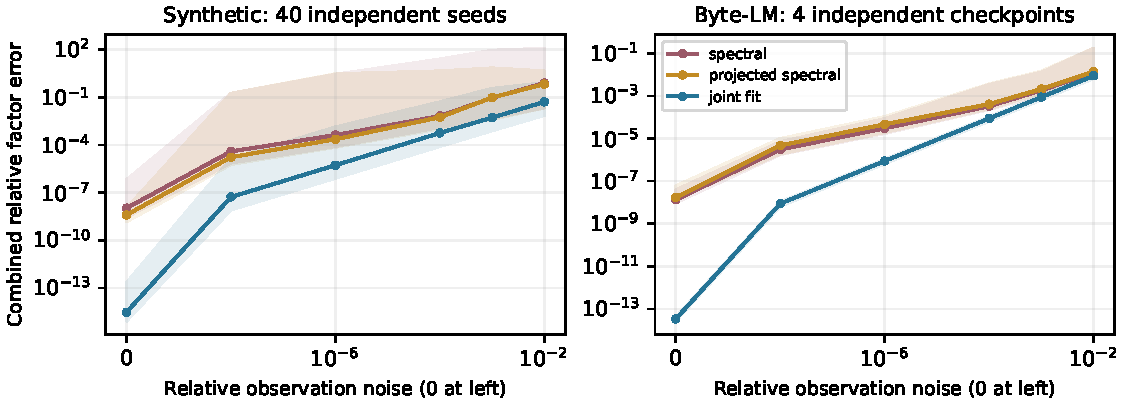
\includegraphics[width=\linewidth]{figures/trusted_recovery.pdf}
\caption{Held-out recovery under simultaneous product and response noise.
Lines show medians and shading the 10th--90th percentiles of the fixed grid,
not confidence intervals. Synthetic aggregation includes all four regimes
and both probe counts; language aggregation includes four checkpoints and
both probe counts. Zero noise is placed at the leftmost plotting coordinate.
Tail failures and diagnostic errors are reported separately.}
\label{fig:trusted-recovery}
\end{figure}

\paragraph{Numerical local separation and reproducibility.}
The 140 synthetic local passes occur in the interior (60) and near-boundary
(80) regimes; there are none in the two rank-contracted regimes.
Only two language outputs pass, both at seed 22.
The pass concerns an estimated-subspace feasible component and has no
unconditional truth-error interpretation.
Raw observations, estimates, starts, failures, diagnostics, source hashes,
calibration thresholds, and per-seed summaries are released under
\texttt{results/trusted\_recovery/}.
Full-coordinate theorem checks are distinct from the recovery experiment.
A separate CPU environment replays the frozen observations; its results
are recorded separately because floating-point optimization need not be
bitwise identical. Across all 1968 cases, good/intermediate/bad classifications
agree for every method. Combined-score acceptance changes in four spectral
and two joint-fit cases; the largest joint-fit error difference is $0.0171$.
Thus environment agreement is assessed explicitly, not inferred from tests.
The release verification rebuilds the reported tables
and checks source and threshold bindings.


\end{document}
